%%%%%%%%%%%%%%%%%%%%%%%%%%%%%%%%%%%%%%%%%%%%%%%%%%%%%%%%%%%%%%%%%%%%%%
% njuthesis 示例模板 v1.2.1 2023-05-03
% https://github.com/nju-lug/NJUThesis
%
% 贡献者
% Yu XIONG @atxy-blip   Yichen ZHAO @FengChendian
% Song GAO @myandeg     Chang MA @glatavento
% Yilun SUN @HermitSun  Yinfeng LIN @linyinfeng
%
% 许可证
% LaTeX Project Public License(版本 1.3c 或更高)
%%%%%%%%%%%%%%%%%%%%%%%%%%%%%%%%%%%%%%%%%%%%%%%%%%%%%%%%%%%%%%%%%%%%%%

%---------------------------------------------------------------------
% 一些提升使用体验的小技巧:
%   1. 请务必使用 UTF-8 编码编写和保存本文档
%   2. 请务必使用 XeLaTeX 或 LuaLaTeX 引擎进行编译
%   3. 不保证接口稳定,写作前一定要留意版本号
%   4. 以百分号(%)开头的内容为注释,可以随意删除
%---------------------------------------------------------------------

%---------------------------------------------------------------------
% 请先阅读使用手册:
% http://mirrors.ctan.org/macros/unicodetex/latex/njuthesis/njuthesis.pdf
%---------------------------------------------------------------------

\documentclass[
    % 模板选项:
    %
    type = master, % 文档类型,默认为本科生
    % degree = academic|professional,        % 学位类型,默认为学术型
    %
    % nl-cover,   % 是否需要国家图书馆封面,默认关闭
    % decl-page,  % 是否需要诚信承诺书或原创性声明,默认关闭
    %
    %   页面模式,详见手册说明
    % draft,                  % 开启草稿模式
    % anonymous,              % 开启盲审模式
    % minimal,                % 开启最小化模式
    %
    %   单双面模式,默认为适合印刷的双面模式
    % oneside,                % 单面模式,无空白页
    % twoside,                % 双面模式,每一章从奇数页开始
    %
    %   字体设置,不填写则自动调用系统预装字体
    latin-font = win,
    cjk-font   = win,
    % math-font  = cambria|newcm|xits, % 完整列表见手册
  ]{njuthesis}

% 模板选项设置,包括个人信息、外观样式等
% 较为冗长且一般不需要反复修改,我们把它放在单独的文件里
% njuthesis 参数设置文件 v1.2.1 2023-05-03

% 一些提醒:
%   1. \njusetup 内部千万不要有空行
%   2. 使用英文半角逗号(,)分隔选项
%   3. 等于号(=)两侧的空格会被忽略
%       3.1. 为避免歧义,请用花括号({})包裹内容
%   4. 本科生无需填写的项目已被特别标注
%   5. 可以尽情删除本注释

% info 类用于录入个人信息
%   带*号的为对应英文字段
\njusetup[info]{
    title = {深度神经网络模型\\分布式训练框架},
    % 中文题目
    % 直接填写标题就是自动换行
    % 可以使用换行控制符(\\)手动指定换行位置
    %
    title* = {A Distributed Training Framework for Deep Neural Network},
    % 英文题目
    %
    author = {崔子寒},
    % 作者姓名
    %
    author* = {Zihan Cui},
    % 作者英文姓名
    % 一般使用拼音
    %
    keywords = {分布式深度学习,模型并行化,深度神经网络},
    % 中文关键词列表
    % 使用英文半角逗号(,)分隔
    %
    keywords* = {{Distributed Deep Learning},{Model Parallelism},{Deep Neural Network}},
    % 英文关键词
    % 使用英文半角逗号(,)分隔
    %
    grade = {2020},
    % 年级
    %
    student-id = {MG20330012},
    % 学号或工号
    % 研究生请斟酌大小写字母格式
    % 本模板并不会自动更正大小写
    %
    department = {计算机科学与技术系},
    department* = {Department of Computer Science and Technology},
    % 院系
    %
    major = {计算机技术},
    major* = {Computer Technology},
    % 专业
    %
    supervisor = {曹春,教授},
    supervisor*= {Professor Chun Cao},
    % 导师全称
    % 使用英文半角逗号(,)分隔中文姓名和职称
    %
    supervisor-ii = {徐经纬,副研究员},
    supervisor-ii* = {Assistant Researcher Jingwei Xu},
    % 第二导师全称
    % 如果确实没有第二导师,不填写即可
    %
    % submit-date = {2022-05-20},
    % 提交日期
    % 格式为 yyyy-mm-dd
    % 不填就是编译当天日期
    %
    %
    % 以下均为研究生项
    %
    % degree = {学术硕士},
    % degree* = {Master of Engineering}
    % 覆盖默认学位名称
    %
    field = {软件方法学与自动化},
    field* = {Software Methodology and Automation},
    % 研究领域
    %
    chairman = {王林章~教授},
    % 答辩委员会主席
    % 推荐使用波浪号(~)分隔姓名和职称
    %
    reviewer = {
        徐峰~副教授,
        李晅松~副教授
    },
    %
    % 答辩委员会成员
    % 一般为四名,使用英文半角逗号(,)分隔
    %
    clc = {TP311.5}, % 软件工程
    % 中国图书分类号
    %
    udc = {004.41}, %软件工程
    % 国际图书分类号
    %
    secret-level = {不涉密},
    % 密级
    %
    defend-date = {2022-05-23},
    % 答辩日期
    % 格式为 yyyy-mm-dd
    % 不填就是编译当天日期
    %
    email = {zihancui@smail.nju.edu.cn},
    % 电子邮箱地址
    % 只用于出版授权书
    %
    %
    % 以下用于国家图书馆封面
    confer-date = {2022-05-22},
    % 学位授予日期
    %
    bottom-date = {2022-05-23},
    % 封面底部日期
    %
    supervisor-contact = {
        南京大学~
        江苏省南京市栖霞区仙林大道163号
    }
    % 导师联系方式
}

% bib 类用于参考文献设置
\njusetup[bib]{
    % style = numeric|author-year,
    % 参考文献样式
    % 默认为顺序编码制(numeric)
    % 可选著者-出版年制(author-year)
    %
    resource = {njuthesis-sample.bib},
    % 参考文献数据源
    % 需要带扩展名的完整文件名
    % 可使用逗号分隔多个文件
    % 此条等效于 \addbibresource 命令
    %
    % option = {
        % doi    = false,
        % isbn   = false,
        % url    = false,
        % eprint = false,
        % 关闭部分无用文献信息
        %
        % refsection = chapter,
        % 将参考文献表置于每章后
        %
        % gbnamefmt = lowercase
        % 使用仅首字母大写的姓名
    %   }
    % 额外的 biblatex 宏包选项
}

% image 类用于载入外置的图片
\njusetup[image]{
    path = {{./logo}},
    % 图片搜索路径
    %
    % nju-emblem = {nju-emblem},
    % nju-name = {nju-name},
    % 校徽和校名图片路径
    % 建议使用 PDF 格式的矢量图
    % 使用外置图片有助于减少编译时间
    % 空置时会自动使用 njuvisual 宏包绘制
    %
    nju-emblem = {nju-emblem-purple},
    nju-name = {nju-name-purple},
    % 替换为紫色版本
    % 这个选项只能填写一次
    % 切换时要注释掉上方的黑色版本
}

% abstract 类用于设置摘要样式
\njusetup[abstract]{
    % toc-entry = false,
    % 摘要是否显示在目录条目中
    %
    % underline = false,
    % 研究生英文摘要页条目内容是否添加下划线
    %
    % title-style = strict|centered|natural
    % 研究生摘要标题样式,详见手册
}

% 目录自身是否显示在目录条目中
\njusetup{
    % tableofcontents/toc-entry = false,
    % 关闭本项相当于同时关闭三个选项
    %
    % listoffigures/toc-entry   = false,
    % listoftables/toc-entry    = false
}

% 为目录中的章标题添加引导线
% \njusetup[tableofcontents/dotline]{chapter}

% math 类用于设置数学符号样式,功能详见手册
\njusetup[math]{
    % style              = TeX|ISO|GB,
    % 整体风格,缺省值为国标(GB)
    % 相当于自动设置以下若干项
    %
    % integral           = upright|slanted,
    % integral-limits    = true|false,
    % less-than-or-equal = slanted|horizontal,
    % math-ellipsis      = centered|lower,
    % partial            = upright|italic,
    % real-part          = roman|fraktur,
    % vector             = boldfont|arrow,
    % uppercase-greek    = upright|italic
}

% theorem 类用于设置定理类环境样式,功能详见手册
\njusetup[theorem]{
    % define,
    % 默认创建内置的七种定理环境
    %
    % style       = remark,
    % header-font = \sffamily \bfseries,
    % body-font   = \normalfont,
    % qed-symbol  = \ensuremath { \male },
    % counter     = section,
    % type        = {...}
    % 以上设置项在重新调用 theorem/define 后生效
}

% footnote 类用于设置脚注样式,功能详见手册
\njusetup[footnote]{
  % style = pifont|circled,
  % 使用圈码编号
  %
  % hang = false,
  % 不使用悬挂缩进
}

% 页眉页脚内容设置
\njusetup{
  % header/content = {
  %     {OR}{\thepage},{OL}{\rightmark},
  %     {EL}{\thepage},{ER}{\leftmark}
  %   },
  % 页眉设置,详见手册
  % 奇数页页眉:左侧章名,右侧页码
  % 偶数页页眉:左侧页码,右侧节名
  %
  % footer/content = {}
}

% 页眉页脚的字体样式
% \njusetformat{header}{\small\kaishu}
% \njusetformat{footer}{}
\njusetformat{chapter}{\zihao{-2}\sffamily\centering}

% 一些灵活调整
% \njusetname{notation}{术语表} % 更改符号表名称
% \njusetname{tableofcontents}{目\qquad{}次} % 更改目录名称
\njusetlength{crulewd}{210pt} % 加长封面页下划线


% 自行载入所需宏包
% \usepackage{subcaption} % 嵌套小幅图像,比 subfig 和 subfigure 更新更好
% \usepackage{siunitx} % 标准单位符号
% \usepackage{physics} % 物理百宝箱
% \usepackage[version=4]{mhchem} % 绘制分子式
% \usepackage{listings} % 展示代码
\usepackage{algorithm,algorithmic} % 展示算法伪代码

% 在导言区随意定制所需命令
% \DeclareMathOperator{\spn}{span}
% \NewDocumentCommand\mathbi{m}{\textbf{\em #1}}

\usepackage{listings}
\usepackage{xcolor}
\usepackage{makecell}
\usepackage{threeparttable}
\usepackage{colortbl}
\usepackage{subcaption}
\usepackage{tabularx}
\usepackage{multirow}
\captionsetup{compatibility=false}


\definecolor{codegreen}{rgb}{0,0.6,0}
\definecolor{codegray}{rgb}{0.5,0.5,0.5}
\definecolor{codepurple}{rgb}{0.58,0,0.82}
\definecolor{backcolour}{rgb}{0.95,0.95,0.92}

\renewcommand{\lstlistingname}{代码}
\lstdefinestyle{mystyle}{
    backgroundcolor=\color{backcolour},   
    commentstyle=\color{codegreen},
    keywordstyle=\color{magenta},
    numberstyle=\tiny\color{codegray},
    stringstyle=\color{codepurple},
    basicstyle=\ttfamily\footnotesize,
    breakatwhitespace=false,         
    breaklines=true,                 
    captionpos=b,                    
    keepspaces=true,                 
    numbers=left,                    
    numbersep=5pt,                  
    showspaces=false,                
    showstringspaces=false,
    showtabs=false,                  
    tabsize=2
}

\DeclareMathOperator*{\argmax}{arg\,max} % Jan Hlavacek
\DeclareMathOperator*{\argmin}{arg\,min} % Jan Hlavacek

\lstset{style=mystyle}

\def\sys{\textsc{NetSplit}}

%%%%%%%%%%%%%%%%%%%%%%%%%%%%%%%%%%%%%%%%%%%%%%%%%%%%%%%%%%%%%%%%%%%%%%%%%%%%%%%
% set up labelformat and labelsep for subfigure 详见: http://www.latexstudio.net/archives/8652.html
\captionsetup[subfigure]{labelformat=simple, labelsep=space}

% 开始编写论文
\begin{document}

%---------------------------------------------------------------------
%	封面、摘要、前言和目录
%---------------------------------------------------------------------

% 生成封面页
\maketitle

% 文档默认使用 \flushbottom,即底部平齐
% 效果更好,但可能出现 underfull \vbox 信息
% 如需抑制这些信息,可以反注释以下命令
% \raggedbottom

\begin{abstract}
  在深度学习领域,随着深度神经网络模型性能的提升,模型的复杂度和大小也在不断增加。单个计算设备已经无法满足大型神经网络模型的训练需求。因此,算法研究者通常使用模型并行化技术,将大型模型划分到多个计算设备上,进行分布式训练。
主流的深度学习框架中,对于模型的划分,仍然依赖使用者手动进行。由于模型结构复杂,加上底层设备的异构性,即使是对于有丰富经验的研究者,手动划分模型也是非常困难的任务。

现有的工作通过强化学习、启发式算法、构建约束优化问题等方法划分模型,但是目前的方法仍然存在一些不足。例如缺少对于底层硬件环境的考虑,对模型训练过程的建模不够精确等。
本文提出了一种针对大型深度神经网络模型的训练框架:\sys{}。具体而言,本文的主要工作包括:
\begin{itemize}
	\item 提出了一种自动化的PyTorch模型分析方法,可以从通用的PyTorch模型中提取出模型计算图的中间表示,并使用静态分析和动态分析的方法分析计算图中每个节点的计算时间和内存占用等元信息。
	\item 提出了一种对底层计算设备之间通信代价的建模方法:针对设备之间可能存在的异构通信链路,自动对设备之间进行点对点通信测试,并建模设备之间的通信代价。
	\item 提出了基于约束优化求解的模型划分方法:基于计算图元信息和设备之间的通信代价模型,构建约束优化问题并进行求解,对模型进行划分。
	\item 在真实场景下对\sys{}进行了实验评估,结果表明,和现有方法对比,\sys{}可以有效提升大型模型的训练效率,缩短训练时间。
\end{itemize}

\end{abstract}

\begin{abstract*}
  In the field of deep learning, with the improvement of the performance of deep neural network models, the complexity and size of the models are also increasing. A single device is no longer capable of training giant neural network models. Therefore, researchers usually use model parallelism to partition large models onto multiple devices for distributed training.

In mainstream deep learning frameworks, the partitioning of models still relies on manual intervention by users. Due to the complexity of the model structure and the heterogeneity of the underlying devices, even for experienced researchers, partitioning model manually is a very difficult task.

Existing work partitions models through reinforcement learning, heuristic algorithms, constructing constrained optimization problems, and other methods, but there are still some shortcomings in these methods. For example, they may not adequately consider the underlying hardware environment, and the modeling of the model training process may not be accurate enough.

To simplify the training process for giant models, especially to provide automated model partitioning functionality, we proposes a training framework for giant deep neural network models: \sys{}. Our contributions include:

\begin{itemize}
\item Implementation of an automated PyTorch model analysis method that can extract the intermediate representation of the model computation graph from a generic PyTorch model and use static and dynamic analysis methods to analyze metadata such as computation time and memory usage for each node in the computation graph.
\item Implementation of a modeling method for the communication cost between underlying devices: for potential heterogeneous communication links between devices, automatic peer-to-peer communication testing is performed between devices, and the communication cost between devices is modeled.
\item Implementation of a model partitioning method based on constrained optimization: based on the metadata of the computation graph and the communication cost model between devices, a constrained optimization problem is constructed and solved to partition the model with the goal of improving training efficiency.
\item Experimental evaluation of \sys{} in real-world scenarios shows that compared to existing methods, \sys{} can effectively improve the training efficiency of large models, resulting in shorter training time.
\end{itemize}

\end{abstract*}

% 生成目录
\tableofcontents
% 生成图片清单
\listoffigures
% 生成表格清单
\listoftables

%---------------------------------------------------------------------
%	正文部分
%---------------------------------------------------------------------
\mainmatter


% 学位论文的正文应以《绪论》作为第一章
\chapter{绪论}\label{chapter_introduction}
\section{研究背景}

近年来,人工智能领域的深度学习技术在各个应用领域都获得了迅速的发展。依赖于大数据时代数据量的爆发式增长,以及高性能计算设备的不断发展,深度神经网络(deep neural networks, DNN)在推荐系统 \upcite{recomendation1,recomendation2},图像识别 \upcite{resnet, imagenet, amoebanet}, 物体检测\upcite{yolo, yolov3} 以及自然语言处理 \upcite{bert,bart} 等应用领域都进行了广泛的应用,并且取得了巨大成功。

如图 \ref{fig:dnn-arch}所示,典型的深度神经网络由若干算子(卷积、池化、全连接等)搭建而成,不同的算子构建成层状结构,层与层被连接在一起,最终构成完整的神经网络模型。
深度神经网络主要依赖反向传播算法 (Back propagation) \upcite{bp}进行训练。以图像识别任务为例,在进行训练前,首先需要将模型的参数加载到内存中,然后针对训练数据,分批次迭代式的读取训练数据和数据对应的标签,首先经过前向传播,将数据输入到模型中,得到模型预测结果。然后将模型预测结果和真实标签输入到损失函数中,计算出损失,再进行反向传播,求解模型参数关于损失的梯度。得到梯度后,再根据优化器 \upcite{adam,rmsprop}的优化策略,对模型参数进行优化。重复上述过程,直到模型收敛。
从反向传播算法的运行过程可以看出,深度神经网络模型的训练是计算密集型任务,训练过程中需要涉及到高维数据的处理,反向传播求导,以及参数优化等。因此,目前的深度神经网络模型的训练通常需要使用专用的高性能计算设备来进行,例如GPU,TPU以及FPGA等 \upcite{tpu-gpu}。
\begin{figure}[h]
	\centering
	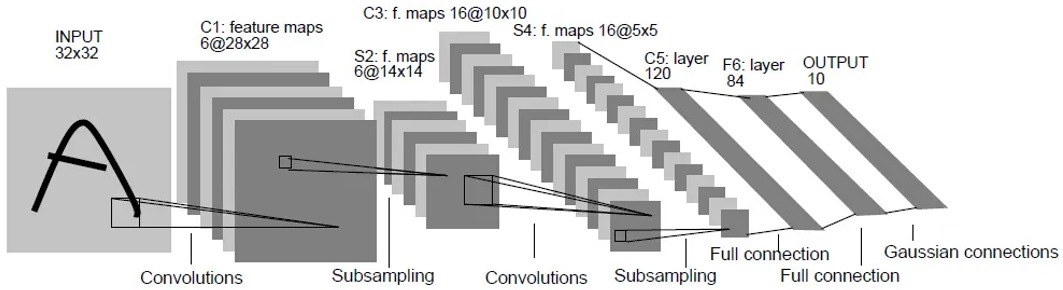
\includegraphics[width=0.8\textwidth]{figure/1-intro/dnn.png}
	\caption{典型深度神经网络结构}
	\label{fig:dnn-arch}
\end{figure}

以深度神经网络为代表的深度学习技术在性能提高的同时,也伴随着模型大小的增加和模型结构复杂度的提升。
以目前主流的高性能计算设备GPU为例,单个设备,无论是运算性能还是设备内存大小,都无法满足模型的训练需求,因此,使用多个设备进行训练,以提升训练效率,已经成为了深度学习领域的最佳实践。
如图 \ref{fig:model-mem} 所示,如果我们使用主流的ResNet-152模型,以$224\times 224$分辨率的输入,在32位浮点精度下,去训练图像识别任务,那么当数据批的大小达到$128$时,就会超过40GB的显存用量,此时,单个GPU设备的显存容量已经很难满足需求。

\begin{figure}[h]
    \centering
    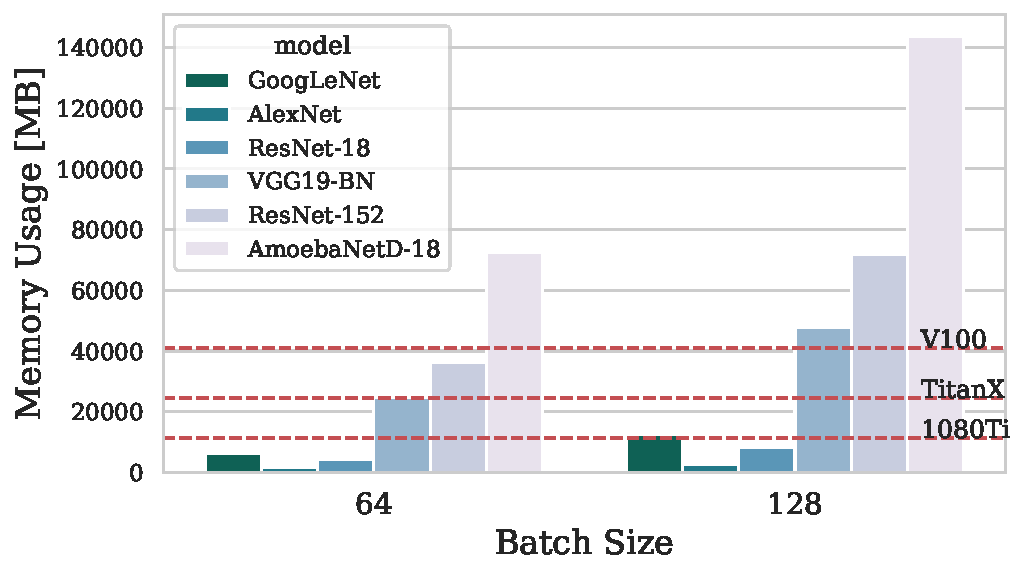
\includegraphics[width=0.8\textwidth]{figure/1-intro/model_mem.pdf}
    \caption{主流计算机视觉模型显存消耗}
    \label{fig:model-mem}
\end{figure}

另一方面,数据集的大小也在不断增大。以ILSVRC-ImageNet2012 \upcite{imagenet} 为例,该数据集的训练集包括1000个分类类别,1300万张训练图片,训练集总大小超过120GB。如果使用单个设备进行训练,将所有图片训练一次(Epoch)需要超过数个小时的时间,而训练需要迭代式进行,往往需要经过多个轮次才能收敛,因此,使用多个计算设备加速训练过程是必要的。

综上所述,使用多个计算设备进行模型训练可以带来以下两点好处:
\begin{itemize}
	\item \textbf{允许训练更大的模型}: 受限于访存速度和制造成本,单个GPU设备的内存容量是有限的。针对大模型,模型的参数会占据大量内存空间,导致没有充足的内存空间去存储训练过程的中间结果、参数梯度等。而对于超大模型,甚至模型参数本身所使用的内存空间就会超过单个设备的内存容量。因此对于这类超大型深度神经网络模型(Giant DNN),使用多个设备进行协同训练是十分必要的。
	\item \textbf{提升训练效率}:模型训练通常使用批处理的方式进行训练,利用GPU的并行计算能力,同时处理一个数据批(Data batch)可以有效加速模型的训练速度,另一方面,使用数据批可以减少对模型参数进行梯度下降优化时的方差,加快收敛速度,现有工作 \upcite{large-batch} 表明,使用大数据批可以更好的代表样本总体,让模型准确的找到收敛方向。而使用大数据批的前提是需要有可用的显存空间,而使用多个GPU设备可以提供更多显存,从而允许算法研究者使用更大的数据批进行训练,提升训练效率,加快模型收敛速度。
\end{itemize}

随着深度学习的不断发展,使用多个设备加速深度神经网络的训练已经成为了最佳实践。
目前主流的开源机器学习框架,如PyTorch \upcite{pytorch} , Tensorflow\upcite{tensorflow} , MXNet\upcite{mxnet} 等,也提供了对多设备并行训练的支持,但是目前,对于超大模型的训练,主流框架多依赖于使用者对多设备协作训练进行手动配置,缺少对于超大模型训练的自动化支持。
尤其是在异构计算集群中,即使对于有经验的算法研究者,也无法总是准确考虑集群中的异构性,设备之间的通信特征以及模型的特点,这导致人工给出的模型训练配置往往不能很好的提高硬件利用率,达到最佳训练效率。因此,设计一种能够自动化完成超大模型端到端训练,自动进行模型划分,多设备协作的训练框架是十分有必要的。


\section{研究现状}
% 
目前,随着各种超大模型被设计出来,利用多设备去并行训练模型,加快模型训练速度的分布式深度学习 \upcite{ddl-survey}成为了机器学习领域的一个重要分支。
针对不同的场景,分布式深度学习有着不同的发展方向。目前,分布式深度学习有三种主要分支:
\begin{itemize}
	\item \textbf{数据并行化 (Data Parallelism, DP)}:数据并行化关注数据吞吐量的提升,也就是单位时间内,模型能够训练的数据样本数目。在数据并行化中,通常存在多个被称作Worker的计算单元,每个Worker使用一个设备,多个Worker之间进行协作完成训练。每个设备持有一个完整的模型副本,Worker使用不同的数据训练本地的模型,并按照一定的策略同步本地模型的参数,这就是数据并行化的思路。
	\item \textbf{模型并行化 (Model Parallelism, MP)}:针对超大模型在单个设备上训练受限的问题,模型并行化被提出,模型并行化也是本文研究的重点。与数据并行化不同,模型并行化针对如何将大型模型划分到多个设备上进行训练,每个设备只持有部分模型,反向传播算法在设备之间分布式运行,设备之间通过通信去传递中间结果以及反向传播过程中产生的梯度。在模型并行化中,由于每个设备只负责部分模型的训练,所以需要按照某些规则对模型进行划分,在划分时,需要考虑设备的负载均衡,避免某个设备的负载较大,成为瓶颈。另一方面,由于模型并行化中,设备之间需要进行大量通信,因此在划分时,也要考虑通信数据量、设备之间的通信链路对于训练效率的影响。
	\item \textbf{混合并行化 (Hybrid Parallelism, HP)}:混合并行化结合数据并行化和模型并行化二者的优势,先将超大模型划分为多个部分,每个部分由若干Worker构成的组进行训练,组内使用数据并行化,加大数据吞吐,组与组之间使用模型并行化,由于结合了二者的优点,因此混合并行化也是针对大模型使用的比较多的一种训练方式。
\end{itemize}

在模型并行化中,由于不同设备之间存在依赖关系,因此设备之间存在互相等待的现象,导致设备利用率低,针对这一问题,研究者专注于设计更好的通信模式,通过流水线的方式,让设备的计算过程和设备之间的通信过程重叠,从而提高设备利用率\upcite{gpipe,pipedream,hetpipe,hippie,dapple}。
Huang \upcite{gpipe} 等人提出了Gpipe技术,通过将数据批进一步细分成更小的微数据批(micro batch),将模型并行化以流水线的形式构建,加速模型并行化训练。
Narayanan \upcite{pipedream} 等人提出了PipeDream,在模型并行化流水线中引入异步计算,在内存中维护了多个版本的模型参数,以空间换时间,进一步提升训练效率。

除了使用流水线技术去改善模型并行化的训练效率外,模型并行化领域的另一个问题是,针对超大模型如何进行模型的划分 \upcite{rl1,rl2,baechi,pesto,rannc}。
Mirhoseini \upcite{rl1,rl2} 等人提出利用强化学习技术进行模型划分,但是随着模型大小的增加和模型复杂度的提升,强化学习收敛慢的问题在面对超大模型时变得更为突出。
Jeon \upcite{baechi} 等人将模型划分问题抽象为处理器调度问题,使用经典的任务调度算法,对模型进行划分。
相比于强化学习,尽管Jeon所使用的任务调度算法运行速度更快,但是其使用的算法是近似算法,在通信受限的场景下近似比较大,无法获得较优的结果。
Hafeez \upcite{pesto} 等人将模型划分问题进行建模,并利用线性规划进行求解。但是该工作只考虑了设备数目为2的简单情况,没有扩展到更多数目的设备,并且在进行问题建模时,没有考虑反向传播开销的影响。

综上所述,现有的模型划分方法仍然存在缺陷,使用模型并行化去训练超大模型时,如何去划分和放置模型仍然是一个亟待解决的问题。

\section{本文工作}
% 实现了xxx系统,使用xxx技术,解决了xxx问题
本文设计并实现了\sys,一种可以进行自动化模型划分与设备放置的超大型神经网络训练框架。
针对神经网络的模型划分问题,\sys 没有对神经网络进行粗粒度的分层切分,而是从神经网络底层的计算图出发,通过将原始模型转换成一种计算图的中间表示,以图的节点为单位对计算图进行细粒度的划分,并从划分后的计算图中重建出与原始模型等价的模型。
为了实现更好的划分效果,\sys 首先对训练使用的硬件环境进行性能测试,主要测试参与训练的设备之间的点对点通信带宽。
接着\sys 会对模型计算图进行分析,通过动态分析和静态分析的方法,获取计算图上每个节点的前向传播用时、反向传播用时、显存用量等模型元信息。
获取元信息之后,\sys 构建出模型划分与设备放置的约束优化问题,以提升训练效率为优化目标,进行求解。
求解完成后,\sys 将划分后的计算图按照求解结果进行设备放置,并基于PyTorch\upcite{pytorch} 实现后续的训练过程。

综上所述,本文提出了一种针对超大型神经网络模型的训练框架\sys,其主要的工作包括:
\begin{itemize}
	\item 基于开源机器学习框架PyTorch,实现了一种可以自动对通用PyTorch模型进行模型划分、设备放置以及训练的框架,可以有效解决大型神经网络在单个设备上难以训练的问题。
	\item \sys 可以根据训练任务所使用的硬件环境,自动化的对硬件进行点对点带宽测试,充分考虑模型并行化任务中,设备之间的通信链路对模型划分效果的影响。
	\item \sys 中实现了一种可以自动将通用的PyTorch模型转化成一种计算图中间表示的功能模块,基于这种计算图的中间表示,\sys 以计算图节点为粒度进行模型划分,相比于以层为粒度进行模型划分,更加细粒度,且更加通用。
	\item 设计了详细的对比实验:分别针对图像分类和图像分割两种任务,选用包括Wide-ResNet152\upcite{resnet} , AmoebaNetD-18\upcite{amoebanet}, U-Net\upcite{unet} 和DeepLab-V3\upcite{deeplabv3}在内的大模型,将\sys 与多种现有的模型划分与设备放置方法进行对比。实验结果显示,相比于现有方法,在不同模型上,\sys 的对于模型训练效率具有至少$4.4\% \sim 14.82\%$的提升。
\end{itemize}

\section{本文组织}
本文剩余章节组织如下:

第二章介绍与本文研究方向相关的技术背景和工作。
首先将介绍本文中出现的一些术语,然后会介绍主流的分布式深度学习技术与发展现状,模型并行化技术的发展,现有的模型划分技术,以及模型训练与计算图方面的工作,并分析大型神经网络模型训练中的难点和挑战。

第三章介绍我们针对大型神经网络模型训练设计的训练框架\sys 以及\sys 中各个功能模块的实现,包含模型转换模块、模型分析模块(显存/计算用时)、通信代价建模模块、计算图划分模块以及最后的模型训练模块。

第四章介绍\sys 中核心算法的实现细节,包括对问题的形式化描述、计算图优化算法、计算图划分算法等。

第五章对\sys 与其他模型划分与设备放置算法的实验进行详细介绍。包括实验对比方法、实验的硬件设置、实验的指标以及实验结果的分析。

第六章对本文工作进行总结,对当前工作中的不足进行分析,并展望本文工作未来的发展。
\chapter{背景知识与相关工作}

\section{模型、计算图与设备}
% 介绍一些专业术语
本节介绍一些与本文工作相关的术语和背景知识。
包括对神经网络模型、计算图以及神经网络训练设备的介绍。
\subsection{模型}
本文中所提到的模型指的是深度神经网络模型(Deep Neural Network, DNN)。
深度神经网络模型来自机器学习的分支领域深度学习,深度学习包括深度神经网络,深度信念网络,深度强化学习等。
深度神经网络模仿人脑中神经元的运作方式,通过激活函数连接模拟神经元。
多层感知机(Multilayer Perceptron, MLP) \upcite{mlp}是最简单的神经网络。
深度神经网络包含一个输入层,一个输出层和至少一层的隐藏层(Hidden Layer)。
每一层都由若干神经元组成,输入数据按照一定规则和神经元的参数进行运算,得到该神经元的输出。
输出经过非线性激活函数后,再作为下一层神经元的输入。
非线性激活函数的存在可以让深度神经网络以任意精度拟合任何函数,为复杂的非线性系统提供建模能力 \upcite{ml-book}。

深度神经网络的建模效果取决于神经元的参数,神经元的参数使用反向传播算法 \upcite{bp}进行训练更新。
反向传播算法的主要过程是首先通过前向传播获取网络的输出,然后选择损失函数(Loss Function),计算网络输出和真实标签的损失(Loss)。
然后反向传播,逐层求解神经元的参数关于损失的梯度,根据选用的优化方法进行梯度下降,更新参数,完成一次训练。
\begin{equation}
	\label{eq:bp}
	W_{i,j}(t+1) = W_{i,j}(t) + \eta \frac{\partial Loss}{\partial W_{i,j}(t)}
\end{equation}

公式 \ref{eq:bp}展示了反向传播算法中一次参数更新的过程。
其中的$Loss$ 代表损失函数计算出的损失,交叉熵损失函数 \upcite{cross-entropy}是一种常用的用于分类任务的损失函数。

\subsection{计算图}
% 深度学习框架的发展

为了帮助深度学习开发者更好的进行模型开发工作,越来越多的开源深度学习框架被设计出来,例如Google开源的Tensorflow \upcite{tensorflow},Facebook开源的PyTorch \upcite{pytorch}等。
随着深度学习框架多年的发展,从方便开发者的角度出发,框架提供更多高层的抽象封装,开发者可以使用高层的应用程序接口迅速搭建自己的模型,而不需要深入到模型底层,处理神经元之间的连接。
而神经元与神经元之间的连接所构成的图,就是深度学习中模型的计算图(Computational Graph)。

最初,开发者需要自己定义计算图中的节点,以及节点与节点之间的连接。
以Tensorflow的发展历程来看,在Tensorflow 1.x版本中,开发者需要手动定义计算图,因此开发一个复杂的模型的十分繁琐,而且静态的计算图给开发调试带来了很多不便。
而在Tensorflow 2.x版本中,则引入了动态图的设定,计算图隐藏在代码中,大大简化了模型的开发流程。
下面是在Tensorflow 1.x和2.x中定义 $a+b$ 的代码片段。

\begin{lstlisting}[language=Python, caption={静态图与动态图的比较}]
# tf 1.x: 手动定义计算图
import tensorflow as tf
a = tf.placeholder(tf.float32, name='var_a')
b = tf.placeholder(tf.float32, name='var_b')
add_op = tf.add(a, b, name='var_c')
sess = tf.InteractiveSession()
init = tf.global_variables_initializer()
sess.run(init)
res = sess.run(add_op, feed_dict={a:2., b:4.,})

# tf 2.x: 自动生成计算图
import tensorflow as tf
a = tf.constant(2.)
b = tf.constant(4.)
print('a+b=', a+b)
\end{lstlisting}


% 模型和计算图的关系
随着框架的发展,已经不需要静态定义完整的计算图,框架可以从开发者的模型定义中动态生成计算图。
在PyTorch和Tensorflow 2.x中,用户通过描述模型的计算过程来定义模型。
计算图则在模型训练时由框架从计算过程的定义中动态生成。
如图 \ref{fig:graph} 所示,这种动态生成计算图的方式帮助开发者屏蔽了底层的细节,提升开发效率,但是也为运行时模型划分带来了困扰。
计算图对用户来说是不透明的,所以从开发者层面无法控制计算图如何被放置,这也是本文工作尝试去解决的问题,
即针对动态图框架,自动的对计算图进行划分。

\begin{figure}[htbp]
	\centering
	\begin{minipage}[b]{0.66\textwidth}
	  \lstinputlisting[language=Python]{figure/2-background/graph.py}
	\end{minipage}
	\hfill
	\begin{minipage}[b]{0.3\textwidth}
	  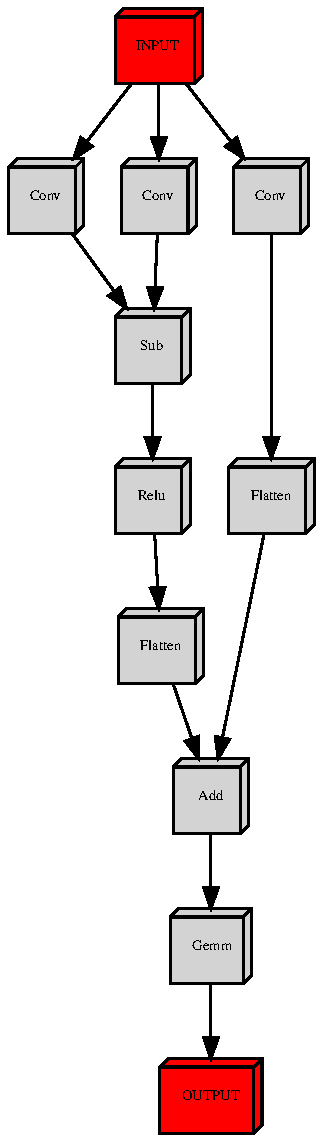
\includegraphics[height=8cm]{./figure/2-background/graph.pdf}
	\end{minipage}
	\caption{模型定义和底层计算图}
	\label{fig:graph}
\end{figure}

\subsection{设备}
% GPU设备的特点
% % 和CPU的区别
% % 内存模型特点
% % 使用CUDA和CUDNN进行计算
% % GPU之间的连接方式介绍, 同个机器上 PCIe, NVLink, 跨节点使用NCCL
本文中所提到的设备特指GPU(Graphics Processing Unit),也就是图形处理器。
最初,GPU主要用于绘制图像和渲染图形,随着高性能计算需求的发展,GPU也发展出了其他的用途,例如用于深度学习中的模型训练、大规模并行处理、以及其他更为严苛的工作负载。
与CPU相比,GPU具有更多的处理单元。
CPU适用于通用的工作负载,特别是对于执行延迟敏感以及对单核性能要求更高的工作负载。
CPU将它数量相对较少的处理器核心集中用于处理单个任务,这让CPU更适合处理串行计算的任务。

通过单指令多数据技术(Single Instruction Multiple Data, SIMD),GPU中的多个计算单元可以同时在不同数据上执行同一条指令,这种架构让GPU适用于处理多维向量数据,同时也让GPU特别适用于进行并行计算。
图 \ref{fig:cpu-gpu}展示了CPU和GPU架构上的区别。
GPU对于高维向量的计算效率也受到了深度学习研究者的青睐,越来越多的深度学习负载运行在GPU上,使用GPU对神经网络和大量高维数据集进行深度学习训练已经成为了深度学习领域的最佳实践。
而GPU厂商也在积极为深度学习提供支持,由Nvidia® 开源的 CUDAToolkit \upcite{cuda}是目前最流行的GPU编程框架,可以让开发者使用GPU来加速自己的程序中的并行计算部分。

GPU通常需要处理大量高维数据,因此读取数据的带宽和数据加载的时延都具有较高的要求。
所以和CPU相比,GPU拥有自己独立的内存,通常称之为显存(Video Memory)。
以Nvidia® V100 GPU为例,它具有900GB/s的显存带宽,而通常的内存带宽只有20GB/s。
但是显存的容量也限制了设备能够运算的数据规模,顶级GPU通常有24~80GB的显存,但是与服务器内存相比,在面对大量数据时,仍然无法满足需求,当可用显存无法满足需求时,通常会引发内存溢出错误(Out of Memory, OOM)。
如何利用多个设备的组合来满足超大模型对的显存需求,也是本文的工作之一。

\begin{figure}[h]
	\centering
	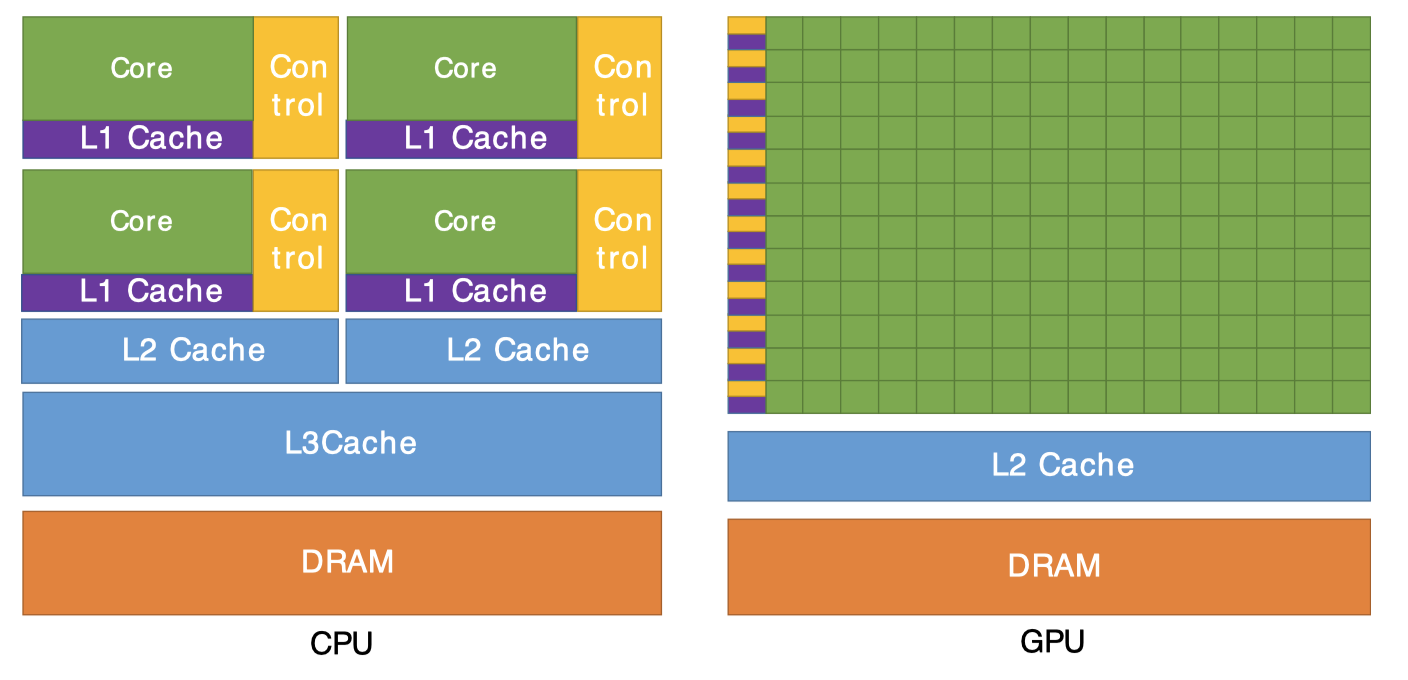
\includegraphics[width=0.85\textwidth]{figure/2-background/cpu-gpu.png}
	\caption{CPU和GPU的架构}
	\label{fig:cpu-gpu}
\end{figure}

受限于单个设备的显存容量和计算能力,多个GPU也常在一起使用,进行并行计算和分布式计算。
在分布式计算过程中,GPU不仅需要处理自己的数据,通常也需要和其他GPU进行数据传输和交换。
使用传统的共享内存或者Socket的方式进行数据传输无法满足GPU之间通信速度的需求。
Nvidia® 开发的NCCL(Nvidia Collective Communication Library) \upcite{nccl}通信库提供了GPU之间进行通信的原语。
NCCL不仅提供了用于点对点通信的原语\texttt{send},\texttt{recv},还提供了例如\texttt{gather},\texttt{broadcast}等集合式通信原语,满足多节点的通信需求。

NCCL从软件层面提供了GPU设备之间通信的功能。在硬件层面,GPU之间有多种通信链路,如图 \ref{fig:gpu-commu} 所示,在计算集群中,GPU之间的通信链路可能有很多不同类型。
在同一个服务器的上的GPU之间可以通过PCIe swtich,也可以使用专有的GPU通信设备NVLink或者NV-Switch \upcite{nvlink}进行通信。
在跨节点通信方面,在非专用集群中,10~25Gbps Ethernet Network Interface Controller(NIC) 仍然是主流选择。
在对通信性能要求较高的场景中,使用 Ehternet NIC则无法满足需求,因此Remote Direct Memory Access(RDMA) \upcite{rdma} 技术被提出。
RDMA协议允许通信实体绕过操作系统内核而直接访问内存中的数据,可以大大提高通信带宽和降低通信延迟,使用RDMA协议的通信设备,例如 Infiniband \upcite{infiniband},可以达到100Gbps的通信带宽。

在分布式计算中,GPU与GPU之间异构的通信链路为系统的设计和工作负载的分发带来了很多挑战。
在分布式深度学习训练中,设备与设备之间需要传递大量的数据。
如果在进行工作负载分发时没有充分考虑集群中通信链路的异构性,则容易导致通信瓶颈的出现,继而影响整个任务的运行效率。
\begin{figure}[h]
	\centering
	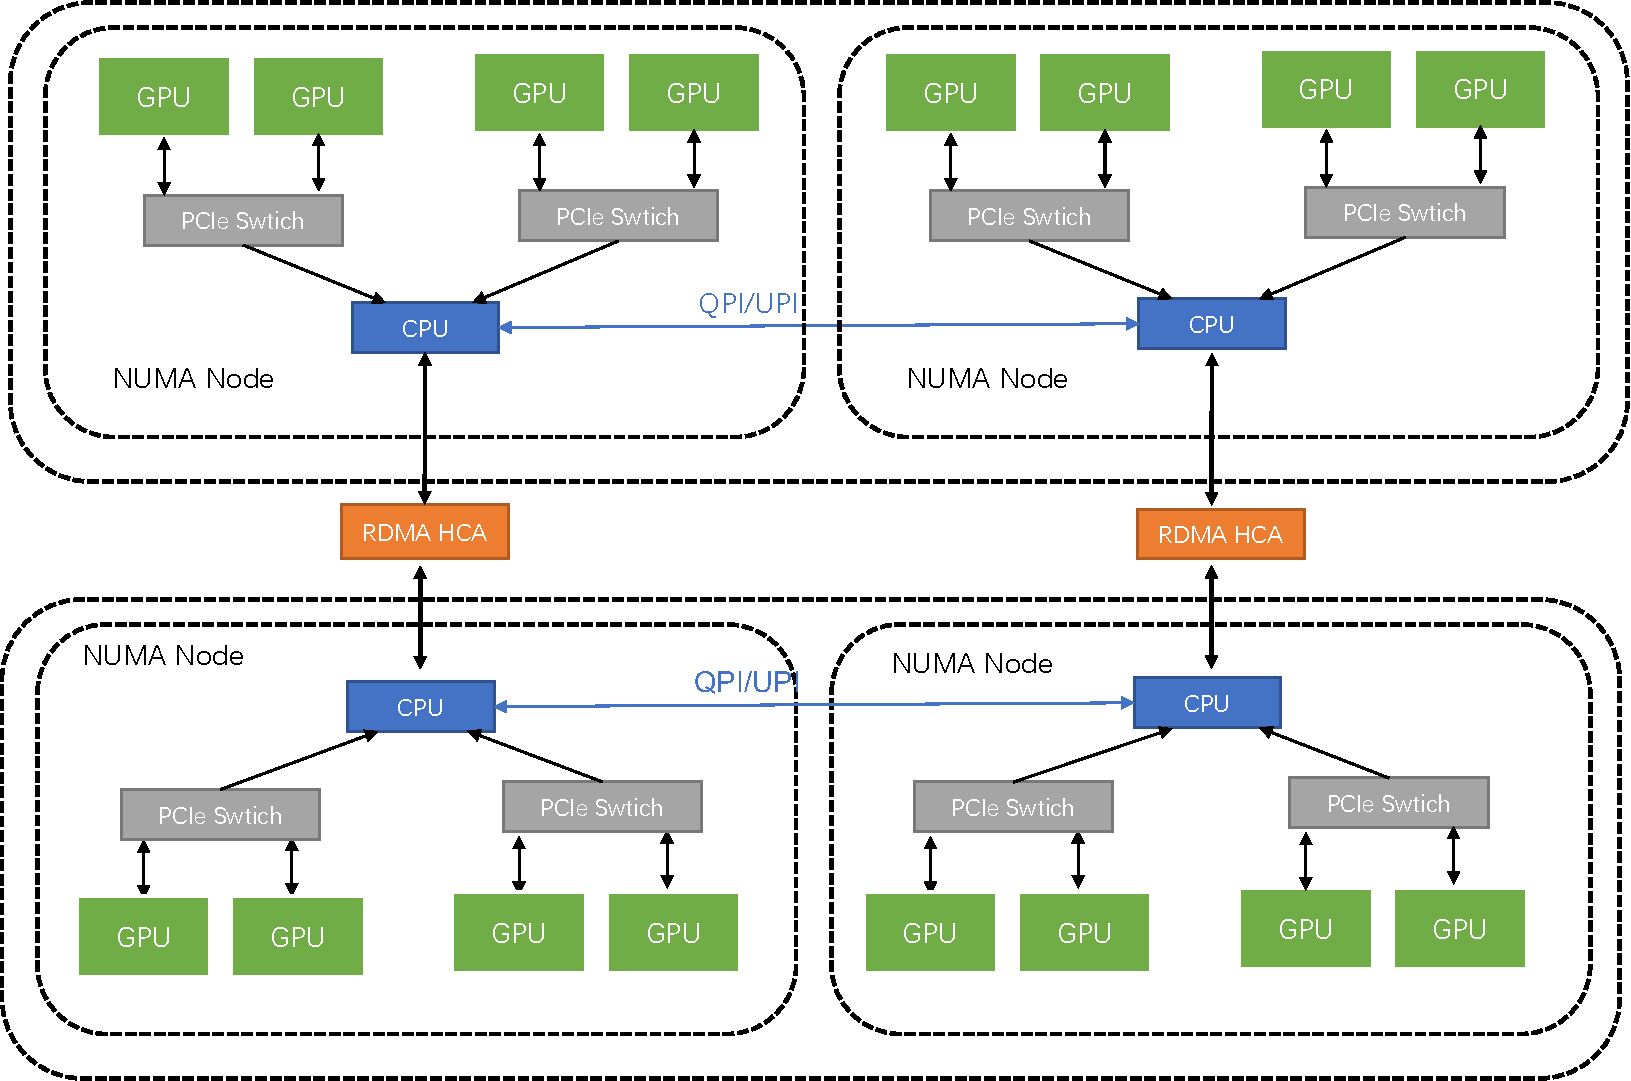
\includegraphics[width=0.9\textwidth]{figure/2-background/commu.pdf}
	\caption{集群中GPU之间通信链路}
	\label{fig:gpu-commu}
\end{figure}

\section{分布式深度学习}
在大数据时代,随着新的应用场景的出现,有更多的数据被收集,而深度学习技术也被广泛的应用在分析数据,构建人工智能应用中, 例如自动驾驶系统 \upcite{self-driving1,self-driving2},AI智能编程助手Copilot \upcite{copilot}等。
目前,面对数据量的增加和模型复杂度的提升,算法研究者们面对的一个重要问题就是如何使用分布式的方式,加速深度神经网络的训练流程。另一方面,模型本身的容量也可能超过单个设备的限制,因此,需要考虑将模型划分到多个设备上,来缓解单个设备的容量不足的问题。
数据并行化(Data Parallelism) \upcite{dp} 与模型并行化(Model Parallelism) \upcite{mp} 分别是分布式深度学习的两种常用的模式,图 \ref{fig:dp-mp} 展示了这两种并行化模式的结构。
% 图 + caption说明
\begin{figure}
	\centering
	\caption{分布式深度学习的两种模式}
	\label{fig:dp-mp}
	\begin{subfigure}[b]{0.4\textwidth}
		\centering
		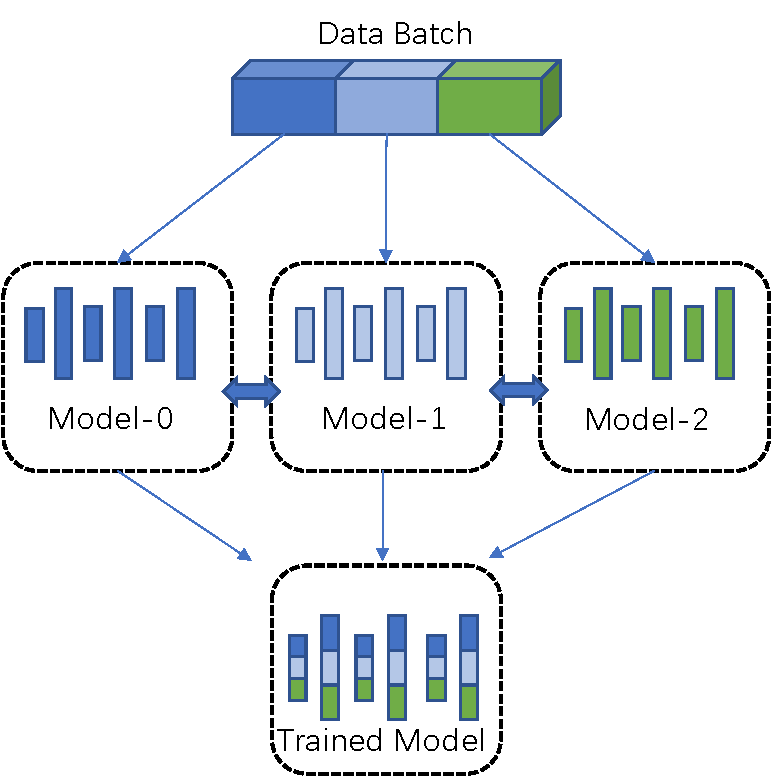
\includegraphics[width=0.85\textwidth]{figure/2-background/dp.pdf}
		\caption{数据并行化}
	\end{subfigure}
	\begin{subfigure}[b]{0.4\textwidth}
		\centering
		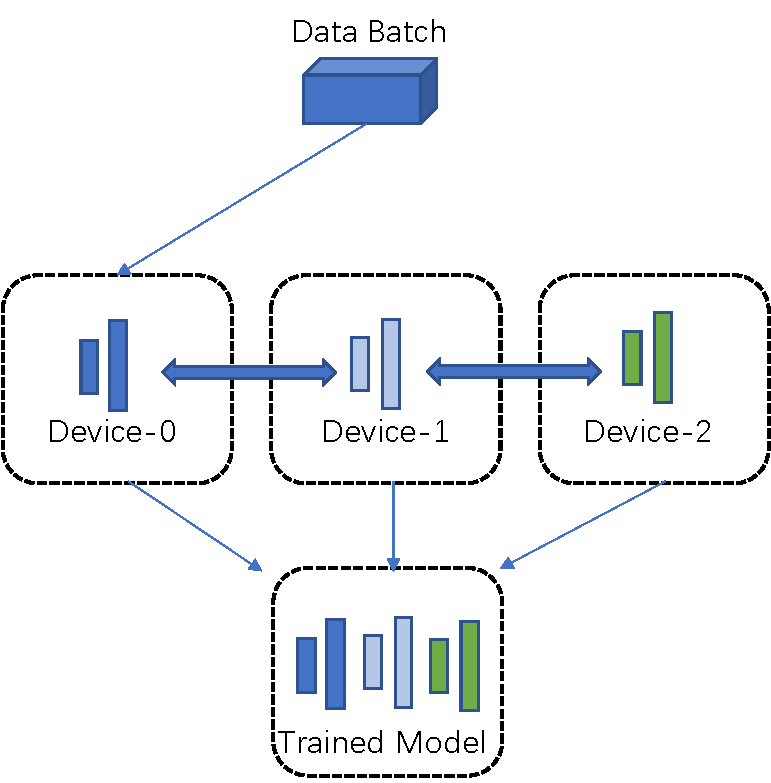
\includegraphics[width=0.85\textwidth]{figure/2-background/mp.pdf}
		\caption{模型并行化}
	\end{subfigure}
	\caption*{a. 数据并行化从训练数据的层面进行并行化,同时训练多个完整的模型副本,每个模型副本使用数据集的一个子集;b. 模型并行化从模型的层面进行并行化,模型并行化将单个模型划分到多个设备上,每个设备负责一部分模型的训练。}
\end{figure}

\subsection{数据并行化}
% 数据并行化的思想
% 数据并行化的两种经典结构 Ring和PS
尽管GPU等专用设备可以加速模型的训练,但是单个设备的算力和容量有限。
利用多个设备通过分布式的方式进行模型训练是加速训练过程的有效方式,多种分布式训练架构被设计出来。
为了应对海量训练数据,数据并行化技术被提出,数据并行化的主要思想为使用多个设备同时训练同一个模型的多个副本。
每个副本使用数据集的一个子集进行训练。
不同的副本周期性通过集合式通信(Collective Communication)进行同步。
在实践中,通常使用数据采样器,采样出一个较大的数据批,然后将数据批按照模型的副本数目进行等分,可以得到多个小数据批。
每个模型副本使用一个小数据批,使用反向传播算法进行训练,然后通过集合式通信,将所有的模型副本的参数梯度求和平均。
每个模型副本使用平均后的梯度来更新模型。

\begin{equation}
	\label{eq:dp}
	\begin{aligned}
		\frac{\partial Loss}{\partial W_{i,j}(t)} =& \frac{\partial \frac{1}{n} \sum_{k=1}^{n} f(x_k, y_k)}{\partial W_{i,j}(t)} = \frac{m_1}{n}\frac{\partial \frac{1}{m_1} \sum_{k=1}^{m_1} f(x_k, y_k)}{\partial W_{i,j}(t)} + \cdots + \frac{m_p}{n}\frac{\partial \frac{1}{m_p} \sum_{k=1}^{m_p} f(x_k, y_k)}{\partial W_{i,j}(t)} \\
		=& \frac{m_1}{n} \frac{\partial L_1}{\partial W_{i,j}(t)} + \cdots + \frac{m_p}{n} \frac{\partial L_p}{\partial W_{i,j}(t)} \\
		=& \frac{1}{p} \sum_{k=1}^{p} \frac{L_k}{\partial W_{i,j}(t)}
	\end{aligned}
\end{equation}

如公式 \ref{eq:dp}所示,
对于大小为$n$的数据批,将其分为$p$份,每份的大小为$m_i,\ 0\le i\le p-1$,每份数据都交给某个设备进行训练。
当满足$m_i=\frac{n}{p}$时,原始数据批关于参数的梯度等于每个小数据批关于参数的梯度的均值。
数据并行化中的关键步骤在于每次反向传播结束后,对不同模型副本的参数梯度进行同步。
参数梯度同步的目的是让模型副本之间共享彼此当前的训练的结果。
从参数梯度同步的架构上,主流的架构有参数服务器架构(Parameter Server, PS) \upcite{ps} 和All-Reduce \upcite{ring} 架构。

\begin{figure}
	\centering
	\begin{subfigure}[b]{0.48\textwidth}
		\centering
		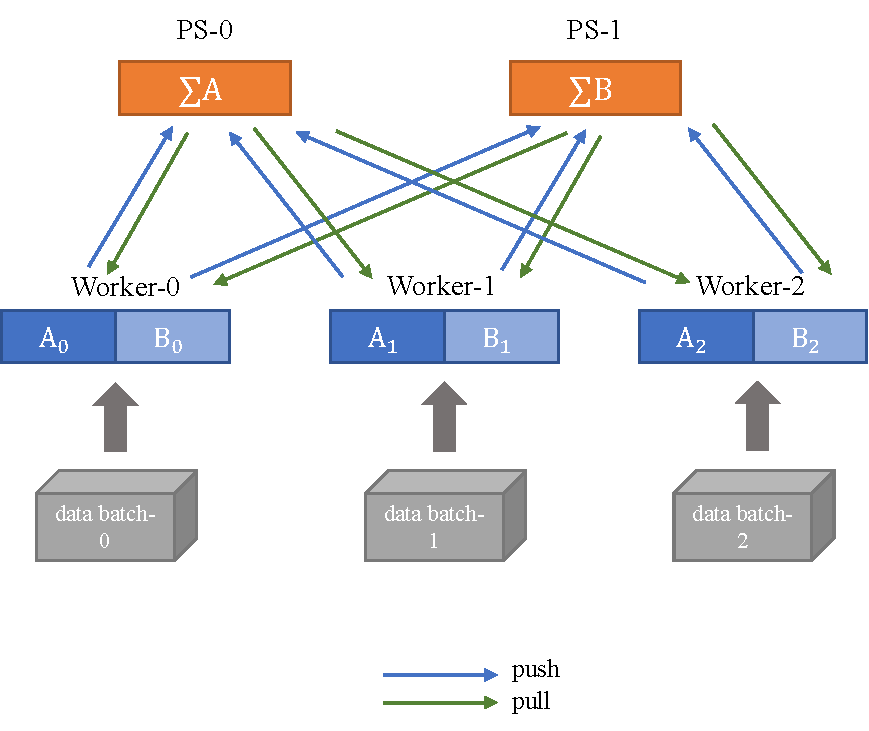
\includegraphics[width=0.95\textwidth]{figure/2-background/ps.pdf}
		\caption{参数服务器架构}
		\label{fig:ps}
	\end{subfigure}
	\begin{subfigure}[b]{0.45\textwidth}
		\centering
		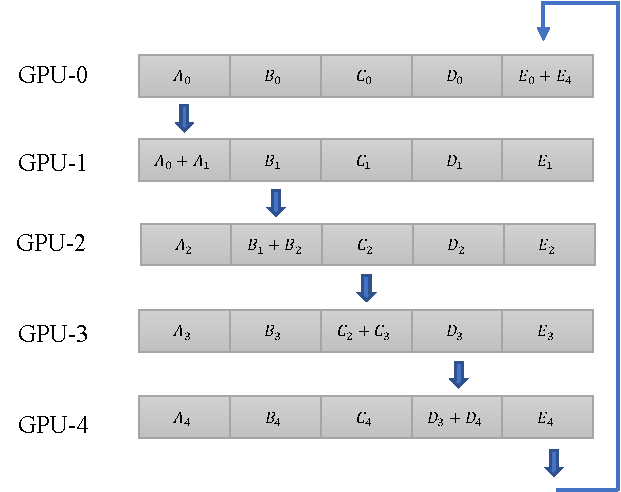
\includegraphics[width=0.95\textwidth]{figure/2-background/ring.pdf}
		\caption{Ring All-Reduce架构}
		\label{fig:ring}
	\end{subfigure}
	\caption{参数服务器架构 vs Ring All-Reduce架构}
	\label{fig:ps-ring}
\end{figure}

\begin{itemize}
	\item \textbf{参数服务器架构}: 参数服务器架构 \upcite{ps} 是最经典的分布式深度学习架构。如图 \ref{fig:ps} 所示,这种架构中,参与训练的节点被从逻辑上划分为了工作节点(Worker Node)和参数服务器节点(PS Node)。
	参数服务器节点的作用是存储模型的参数状态。
	工作节点的职责是进行模型的训练。
	当工作节点完成本地模型的训练后,会将本地最新的模型参数推送到参数服务器。
	参数服务器在接收到工作节点推送的模型参数后,会更新其存储到全局参数。
	然后工作节点再从参数服务器上拉取模型的全局参数。
	参数服务器可以有多个,每个参数服务器存储一部分模型。
	这种架构的优点在于工作节点和参数服务器节点的数量可以根据具体的硬件环境灵活调整,这让参数服务器架构拥有灵活的扩展能力。
	缺点在于参数服务器架构是中心化的架构,通信在参数服务器节点和工作节点之间频繁发生,而参数服务器节点往往需要同时和多个工作节点进行通信,容易导致通信瓶颈的产生。
	在参数服务器架构的基础上,衍生出多种改进版本。如BytePS \upcite{byteps},ElasticPS \upcite{elasticps},ParameterHub \upcite{pshub}等。

	\item \textbf{All-Reduce架构}: 以Ring All-Reduce \upcite{ring} 为代表的All-Reduce架构是一种去中心化的参数同步架构。
	如图\ref{fig:ring} 所示,在All-Reduce架构中,参与训练的计算节点被组织成为一个逻辑环。
	环上的每个节点都有唯一的前驱和后继,通信只发生在节点和前驱/后继之间。
	由于环上所有节点都是处于对称地位,所以每个节点的通信量是相同的,这也避免了参数服务器架构中的通信瓶颈的出现。
	每个节点在训练完成后,都将本地的模型参数分块后,在环上传递给自己的后继。
	在节点数目为$n$时,经过$2(n-1)$ 次通信就可以完成参数的同步。

	\item \textbf{Peer-to-Peer 架构}: 相比于对架构有严格限制的参数服务器架构和All-Reduce架构,Peer-to-Peer 架构采取了一种完全分布式的方式。每个工作节点都有完整的模型副本,工作节点之间直接进行点对点通信。
	这种方式具有更高的可扩展性,而且可以很好的处理分布式系统中的单点故障问题。
	受到这种思想的启发,Gossip Learning \upcite{gossip-learning} 被提出,并且用于分布式深度学习。
	Gossip Learning按照点对点通信网络中进行独立随机游走的想法构建。
	每个结点更新本地参数时,按照随机游走的方式,随机选取一组相邻节点,并将相邻节点的模型参数合并到本地。

\end{itemize}

从参数梯度同步的策略上,可以分为批同步方式(Bulk Synchronous Parallel, BSP),异步方式(Asynchronous Parallel, ASP)以及延迟同步方式(Stale Synchronous Parallel, SSP)。
\begin{itemize}
	\item \textbf{批同步策略(BSP)}: BSP策略 \upcite{bsp}是最简单的一种同步策略。
	使用BSP参数同步策略可以有效保证参与同步的参数的版本的一致性。
	经典的大数据并行计算架构MapReduce \upcite{mr}就使用了BSP同步策略。
	BSP通过对各个参与模型训练的节点的本地计算的进度进行同步来保证一致性,
	在每次迭代中,参与训练的工作节点首先读取训练数据,执行本地训练,当所有工作节点完成本地训练后,才进行接下来的参数同步。
	BSP的优点在于提供了对模型训练收敛性的保证,但是缺点是引入的同步障(Synchronization Barrier)容易造成工作节点之间的相互等待,运行速度快的节点需要等待运行速度慢的节点完成,一定程度上会影响训练的效率 \upcite{projadam}。
	BSP策略既可以用于参数服务器架构,也可以用于All-Reduce架构。
	\item \textbf{异步同步策略(ASP)}: ASP策略允许参与同步的节点不需要进行互相等待而可以并行通信。由于ASP中没有同步障,不存在相互等待,所以ASP策略下,单次同步非常快。
	但是ASP策略的缺点是模型可能永远不会收敛,在ASP同步策略中,参与同步的模型参数版本的差距可以是任意大,这将导致模型收敛慢或者无法收敛。
	\item \textbf{延迟同步策略(SSP)}: SSP策略是 \upcite{ssp}是对BSP和ASP的一种折衷。
	SSP允许参与同步的模型的参数版本的差距在一定范围内,该范围通过staleness 参数控制。
	如果参与同步的模型的参数版本的差距超过了限制,则退化为BSP,使用旧版本的模型参数进行同步。
	SSP的优点是缓解了BSP中的节点互相等待的情况,运行较快的节点不需要总是等待其他节点。
	SSP的缺点在于虽然SSP保证模型的收敛性,但是当staleness较大时,仍然可能影响收敛的效率。

\end{itemize}

\subsection{模型并行化}
% 模型并行化思想
数据并行化从数据角度进行并行,通过多路数据流进行训练加速。
而模型并行化从模型的角度进行划分,主要解决单个设备的内存有限,无法容纳大型模型的所有参数的问题。
如图 \ref{fig:dp-mp} 所示,在模型并行化中,模型被划分到多个设备上,每个设备负责部分模型的训练。
设备与设备之间通过相互通信传递前向传播的输入和反向传播的梯度,当训练完成后,所有设备上的模型组合在一起,得到完整的模型。
流行的深度学习框架如Tensorflow,PyTorch等,对数据并行化具有较为完善的支持,但是对模型并行化的支持有限,因为模型并行化中涉及到如何将模型划分到多个设备上,目前在PyTorch 1.13版本中引入了模型并行化的功能 \upcite{pytorch-pipeline},但是仍然依赖用户手动对模型进行划分。

% 介绍Gpipe等流水线并行化技术
在模型并行化研究领域,如何提高设备的计算利用率是另一个研究重点,由于模型并行化的特点,不同的设备之间有相互依赖。
设备之间通过通信传递数据,而设备的计算和通信过程无法重叠,当设备训练完本地的部分模型后,会进入通信过程,等待其他设备接受输出,以及等待来自其他设备的输入,如图 \ref{fig:mp-time} 所示,模型并行化中存在着设备利用率低下的问题。

\begin{figure}[h]
	\centering
	\begin{subfigure}[b]{0.85\textwidth}
		\centering
		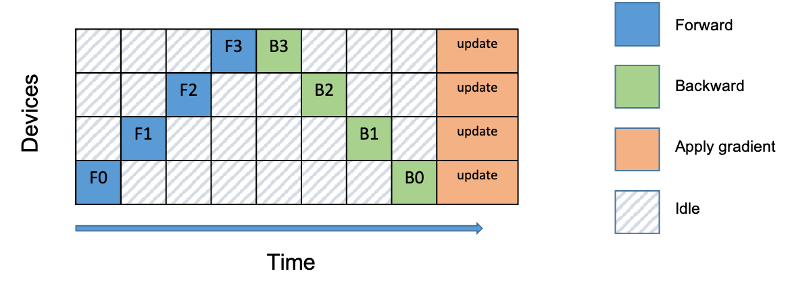
\includegraphics[width=0.85\textwidth]{figure/2-background/mp-time.png}
		\caption{模型并行化}
		\label{fig:mp-time}
	\end{subfigure}
	\begin{subfigure}[b]{0.95\textwidth}
		\centering
		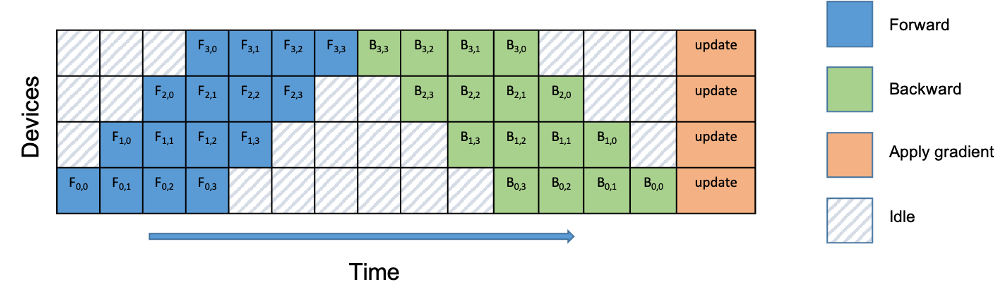
\includegraphics[width=0.85\textwidth]{figure/2-background/gpipe.png}
		\caption{流水线优化}
		\label{fig:gpipe}
	\end{subfigure}
	\caption{模型并行化 vs 流水线并行化}
	\label{fig:mp-gpipe}
\end{figure}

为了缓解模型并行化中,各个设备之间由于相互依赖导致的设备利用率低的问题,Huang等人提出了Gpipe \upcite{gpipe}。
Gpipe使用流水线技术优化模型并行化的过程,如图 \ref{fig:gpipe}所示,对于每个数据批,Gpipe将其进一步细分为微数据批(Micro Batch)。
某个设备处理完当前的微数据批后,将输出发送给下一个设备,然后立刻开始下一个微数据批的处理。
反向传播的过程也是类似,直到一个完整的数据批被处理完成,才更新所有的模型参数。
同时,Gpipe也提出了利用“重计算”优化显存使用。
设备不再暂存当前数据的输出结果,而是在进行反向传播计算梯度时,再重新执行前向传播过程,获取输出,再计算梯度。

除了Gpipe,使用流水线优化模型并行化的工作不断涌现。
Narayanan 等提出了PipeDream \upcite{pipedream}, 一种异步的流水线策略。
在PipeDream中,每个设备上同时维护多个模型参数的版本,当数据批到达时,选用最新的模型参数版本进行训练。
并且在之后的反向传播过程中,也使用相同版本的参数,以保持参数一致性。
Fan等人提出了Dapple \upcite{dapple}。Dapple组合了数据并行化和模型并行化。
模型被划分到多个设备组上,设备组之间使用模型并行化,设备组内部使用数据并行化。
此外Dapple还使用Early Backward技术来节省显存,通过调度每个设备进行前向传播和反向传播的顺序,优先让设备进行当前数据批的反向传播,释放掉中间结果的显存。

本小节中介绍了模型并行化以及在模型并行化上进行优化的一些相关工作。
这些工作主要从模型并行化的计算模式上进行优化,和本文工作\sys{} 中涉及的模型划分是正交的,属于不同的优化方向。
在\ref{sec:partition} 节中,将会介绍有关模型并行化中,进行模型划分的一些相关工作。


\section{模型划分技术}
\label{sec:partition}
% 介绍模型划分技术
% 维度: layer-level和operator level
% 比较,说明operator level粒度细,效果好
% 方向:
% 1. RL 
% 2. 经典算法
% 3. 约束优化
% 4. 启发式

\begin{lstlisting}[language=Python, caption={PyTorch 1.13中的流水线并行化}]
 # 分布式训练环境初始化
 os.environ['MASTER_ADDR'] = 'localhost'
 os.environ['MASTER_PORT'] = '29500'
 # 构建流水线
 fc1 = nn.Linear(16, 8).cuda(0)  # 划分到GPU-0
 fc2 = nn.Linear(8, 4).cuda(1)   # 划分到GPU-1
 model = nn.Sequential(fc1, fc2)
 model = Pipe(model, chunks=8)
 input = torch.rand(16, 16).cuda(0)
 output_rref = model(input)
\end{lstlisting}


上述代码展示了来自PyTorch官方文档\footnote[1]{https://pytorch.org/docs/stable/pipeline.html\#torch.distributed.pipeline.sync.Pipe}关于如何将模型划分到多个设备上进行流水线训练的例子。
在这个例子中,首先设置了环境变量,用来指定分布式训练时,需要进行RPC通信的地址。
在5至7行,是模型定义和模型划分,用户需要手动为模型中的每一层分配CUDA设备,在例子中,全连接层fc1被划分到了0号设备,fc2被划分到了1号设备。
在8至10行,被划分好的模型被\texttt{Pipe}包装,进行训练。
\texttt{Pipe}只能接受\texttt{nn.Sequential},也就是模型必须可以表达为连续的若干层,才可以进行进一步的训练。
在原生的PyTorch中,只支持这种对模型进行分层手动划分的方式。
这种方式粒度较粗且缺乏通用性,很难应用到复杂模型上,因为复杂模型难以使用简单的分层结构进行描述。
尽管按层划分是一种可行的方案,但是其仍有如下的不足:
\begin{itemize}
	\item 限制了使用者定义模型的方式:按层划分只接受可以表示为连续若干层的模型,例如在PyTorch中,这类模型通常定义为\texttt{nn.Sequential},每一层只有一个前驱和一个后继。
	在进行划分时,连续的若干层会被划分到一个设备上。
	然而在实际进行模型开发时,模型并不总是可以表示为连续的若干层,例如一些结构比较复杂的模型,在PyTorch中通常会被定义为 \texttt{nn.Module},而这类模型并不支持按层划分。
	\item 按层划分难以达到最优的负载均衡:在模型并行化训练中,由于参与训练的设备之间存在依赖关系,因此需要谨慎的划分模型,让不同设备具有近似的负载,来避免负载不均。而层的定义也依赖于开发者,这容易导致层与层之间的大小(参数量、运算量)区别很大,例如在 基于BERT \upcite{bert} 的模型中,模型的最后一层占据了整个模型40\%的计算时间,对于这种巨大的层,还需要进一步的划分,才能保证不同设备的负载均衡。
	\item 按层划分是一种粗粒度划分方式:即使模型可以被表示为若干连续的层,那么对这些层进行划分的前提是层数大于设备数目,因为每个设备只少要被分到一层模型,但实际情况不总是如此。
\end{itemize}

在运行时,模型会被执行框架编译为计算图,再由运行时进行执行。
直接对计算图进行划分,也就是按照计算节点划分(Operator-wise) 可以有效避免按层划分的缺点。
从计算图层面对模型进行划分的工作有如下的方向:
\begin{itemize}
	\item \textbf{基于强化学习的方法}:Mirhoseini等提出了基于强化学习的计算图划分方法 \upcite{rl1,rl2}。
	Mirhoseini 使用的模型是NLP领域常用的Seq2Seq \upcite{seq2seq} 模型,并在该模型中加入了注意力机制。
	Seq2Seq模型由编码器(Encoder)和解码器(Decoder)两部分组成,编码器和解码器都使用LSTM(Long short-term memory) \upcite{lstm} 实现。
	该方法首先将计算图中的每个节点都进行编码,编码内容包括节点的类型,节点的输出大小,节点的邻接表。然后将节点编码序列输入到模型中,由模型输出每个节点的放置结果,也就是节点被放置到的设备编号。
	使用强化学习方法的缺点是需要很长的训练时间。
	\item \textbf{基于任务调度的近似算法}:Jeon等提出了使用基于任务调度的近似算法进行计算图的划分 \upcite{baechi}。
	计算图中的每个节点可以看作具有不同执行时长的任务,设备可以看作运行任务的处理器。
	节点之间的边则定义了任务的依赖,因此,从任务调度的角度,可以将计算图的划分问题建模为在有限个处理器上调度多个具有不同运行时长且具有依赖关系的任务。
	Jeon等使用经典的任务调度近似算法 \upcite{sched} 进行计算图的划分,包括最短任务优先(Earliest Task First, ETF) 和最短通信时间(Small Communication Time, SCT) 算法。
	\item \textbf{基于约束优化的方法}:计算图的划分问题在理论上被证明是NP-hard问题 \upcite{sched} ,因此无法找到多项式时间内的确定性算法对其进行求解,找到给定计算图和给定设备下的最优计算图划分。
	尽管Jeon等提出的近似算法可以快速得到近似解,但是由于算法近似比的限制,往往近似解无法取得和最优解一样的好结果。
	为了能够获得更好的划分结果,Hafeez等 \upcite{pesto} 将计算图的划分问题建模为一组约束优化,并使用高性能约束优化器进行求解。
	实验证明,该方法相比于强化学习和近似算法,可以得到更好的划分结果。

\end{itemize}

\section{本章小结}

本章首先对本文中出现的若干术语和概念,如模型、计算图和设备进行了详细的介绍。
然后介绍了分布式深度学习的发展和目前的两种主要模式,包括数据并行化和模型并行化。
有关数据并行化,介绍了其适用场景和主流架构,包括参数服务器架构和All Reduce架构,并对两种架构进行了对比。
有关模型并行化,介绍了模型并行化和数据并行化的区别,以及适用场景,并介绍了对于模型并行化的流水线优化技术。
最后,介绍了模型并行化中一个重要问题,也就是模型的划分问题。比较了分层划分和计算图划分两种方式,并介绍了目前对于模型划分的三种工作方向。
下一章将介绍我们针对大型神经网络模型训练提出的\sys{}框架的设计和各个功能模块的实现。 
\chapter{研究动机与框架概览}
\label{chapter:analysis}

为了帮助研究者更方便的设计和实现神经网络模型,多种流行的神经网络框架被设计出来,并得到了广泛的使用,例如PyTorch, Tensorflow等。
但是目前的框架对于模型并行化训练的支持较为有限,仍然需要研究者手动对模型进行划分,手动管理模型和设备的映射关系。
针对当前框架的不足,我们基于PyTorch设计并实现了\sys{}。
\sys{}提供了对大型神经网络的自动化划分和训练功能,尽可能的简化了大型神经网络的训练流程。
本章节首先介绍大型神经网络训练中的一些难点(\ref{sec:difficulties})和问题分析(\ref{sec:analysis}),然后介绍我们针对大型模型训练所设计的\sys{}框架的整体架构(\ref{sec:design})。

\section{难点与挑战}
\label{sec:difficulties}

超大型神经网络模型由于其含有巨量的参数,因此通常需要将模型划分到多个设备上,使用模型并行化的方式进行分布式训练。
因此,训练超大型模型时,首要难点是如何进行模型划分。
尽管目前PyTorch 1.13 中支持了模型并行化和流水线优化,但是对于模型的划分,仍然依赖于使用者进行手动划分。
另一方面,PyTorch中,对于模型划分的支持只在按层划分的粒度。
\begin{lstlisting}[language=Python, caption={PyTorch 1.13中的流水线并行化}]
 # 分布式训练环境初始化
 os.environ['MASTER_ADDR'] = 'localhost'
 os.environ['MASTER_PORT'] = '29500'
 torch.distributed.rpc.init_rpc('worker', rank=0, world_size=1)
 # 构建流水线
 fc1 = nn.Linear(16, 8).cuda(0)  # 划分到GPU-0
 fc2 = nn.Linear(8, 4).cuda(1)   # 划分到GPU-1
 model = nn.Sequential(fc1, fc2)
 model = Pipe(model, chunks=8)
 input = torch.rand(16, 16).cuda(0)
 output_rref = model(input)
\end{lstlisting}


上述代码展示了来自PyTorch官方文档\footnote[1]{https://pytorch.org/docs/stable/pipeline.html\#torch.distributed.pipeline.sync.Pipe}关于如何将模型划分到多个设备上进行流水线训练的例子。
在这个例子中,首先设置了环境变量,用来指定分布式训练时,需要进行RPC通信的地址。
在6-9行,是模型定义和模型划分,用户需要手动为模型中的每一层分配CUDA设备,在例子中,全连接层fc1被划分到了0号设备,fc2被划分到了1号设备。
在10-12行,被划分好的模型被\texttt{Pipe}包装,进行训练。
\texttt{Pipe}只能接受\texttt{nn.Sequential},也就是模型必须可以表达为连续的若干层,才可以进行进一步的训练。
在原生的PyTorch中,只支持这种对模型进行分层手动划分的方式。
这种方式粒度较粗且缺乏通用性,很难应用到复杂模型上,因为复杂模型难以使用简单的分层结构进行描述。

相比于粗粒度的分层划分,主流的模型划分的工作\upcite{baechi,pesto,rl2,rl1} 针对Tensorflow框架,从模型计算图的角度对模型进行划分。
在Tensorflow 1.x中,用户通过定义计算图来定义模型,计算图可以通过静态分析获得。
而在PyTorch中,用户定义模型和计算图之间仍然具有较大的区别。
PyTorch框架直接对模型的定义代码进行解释执行,在运行时再获取模型的节点(Operator)、节点之间的依赖关系,从而得到运行时动态构建的计算图。
针对PyTorch中大模型的模型并行化训练,我们希望自动化的完成计算图的获取,同时,在对计算图进行划分时,也需要知道每一个节点的内存需求,从而确保划分后,每个设备上分到的节点使用的内存容量不超过设备限制。另外也需要获取每个节点的执行时间,节点与节点之间的通信时间等,来指导模型的划分。在这一过程中,有如下的难点:
% 同时,在对计算图进行划分时,也需要知道每一个节点的内存需求,从而确保划分后,每个设备上分到的节点使用的内存容量不超过设备限制。
% 另外也需要获取每个节点的执行时间,节点与节点之间的通信时间等,来指导模型的划分。
% 1. 用户定义
% 2. 如何获取
% 3. 如何划分模型
\begin{itemize}
	\item \textbf{用户定义模型预处理}:在PyTorch中,用户通常使用高层应用程序接口定义模型。这种高层级的模型在进行训练时,会由训练框架编译为运行时模型。
	用户定义的高层级的模型具有强大的表达能力,方便用户使用简单的代码定义出复杂的模型。
	但是这种高层级的模型往往难以划分。
	因此,需要对用户模型进行一定的预处理,在不改变模型的原有结构和功能的前提下,将模型转化为容易划分的形式。
	% 模型的划分就是计算图的划分,因此我们需要将用户的模型转换为一种计算图的中间表示,划分完成后,再根据划分结果,将中间表示转换回可以进行训练的模型。
	\item \textbf{模型的复杂性}:大型神经网络模型具有复杂的结构,巨大的参数量和很深的网络层次,因此其对应的计算图也有很多节点。每个节点都会进行很多计算,节点需要显存来储存参数,同时节点与节点之间的中间结果也会占用显存,繁多的节点和中间结果让对模型进行分析变得十分困难。
	\item \textbf{硬件环境的复杂性和异构性}:非专有集群中各个设备的型号可能不同,因此它们之间的计算速度和能力也有所不同,在分布式训练中需要控制各个节点之间的计算时间和通信开销,否则会造成任务分配、数据传输等方面的效率问题。
	\item \textbf{模型划分方法的设计}:尽管流水线并行化工作\upcite{gpipe,pipedream,dapple,hippie}被证明可以有效的提高模型并行化中的设备利用率和训练效率,合适的模型划分对于进一步提升训练效率也十分重要。
	通过合理的模型划分,可以有效减少设备之间通信时间,均衡负载,提升训练速度,也可以避免设备出现内存溢出问题。
\end{itemize}


\section{问题分析}
\label{sec:analysis}
% 

针对大型神经网络模型训练中的难点,我们可以将大型神经网络模型的训练问题分解为几个子问题。
\begin{itemize}
	\item \textbf{模型结构理解}:在模型并行化中,需要将模型划分到多个设备上进行训练。这需要让框架对模型的结构有深刻的理解。
	对于现代的深度学习框架来说,通常使用计算图这种中间表示(Intermediate Representation, IR) 来描述运行时的模型。
	我们需要对用户定义的高层级的模型进行分析,从用户的代码中提取出模型的结构信息,并将其转化为计算图这种易于划分的中间表示。我们将这一过程称之为模型结构的理解。
	\item \textbf{模型元信息提取}:在完成“模型结构理解”后,可以得到模型的计算图表示。但是为了下一步的模型划分,还需要对计算图进行分析。框架应该可以自动的提取出会对训练效果产生影响的模型元信息,包括计算图中每个节点的显存需求和计算代价。模型的划分可以简化为寻找计算图中节点到设备的映射,每个设备都会被分配到计算图上的若干节点。因此首先需要保证设备上被分配到的节点使用的显存不会超出设备总显存,从而导致内存溢出问题。
	此外,还需要得知每个节点的前向传播/反向传播用时,节点之间传输的数据量等信息,才能更好的指导模型的划分。
	\item \textbf{训练环境分析}:针对底层硬件设备的异构性,我们需要构建对训练环境进行分析的模块。设备的显存容量制约模型的划分,而设备之间的通信会影响训练的效率,所以我们需要对训练环境进行分析,提取出设备信息,并且对设备之间的通信速度进行分析,减少通信因素对于训练效率的影响。
	\item \textbf{模型划分与训练}:我们需要结合模型结构,模型元信息和具体的训练环境,为模型寻找最优的划分方案,提升训练效率。
	此外,由于划分在计算图层面进行,我们还需要根据对计算图的划分结果,对计算图进行放置,并且对于跨设备的节点,处理它们之间的通信。
	最终完成对划分后的模型的训练。
\end{itemize}

\section{\sys{} 设计}
\label{sec:design}

\begin{figure}[h]
	\centering
	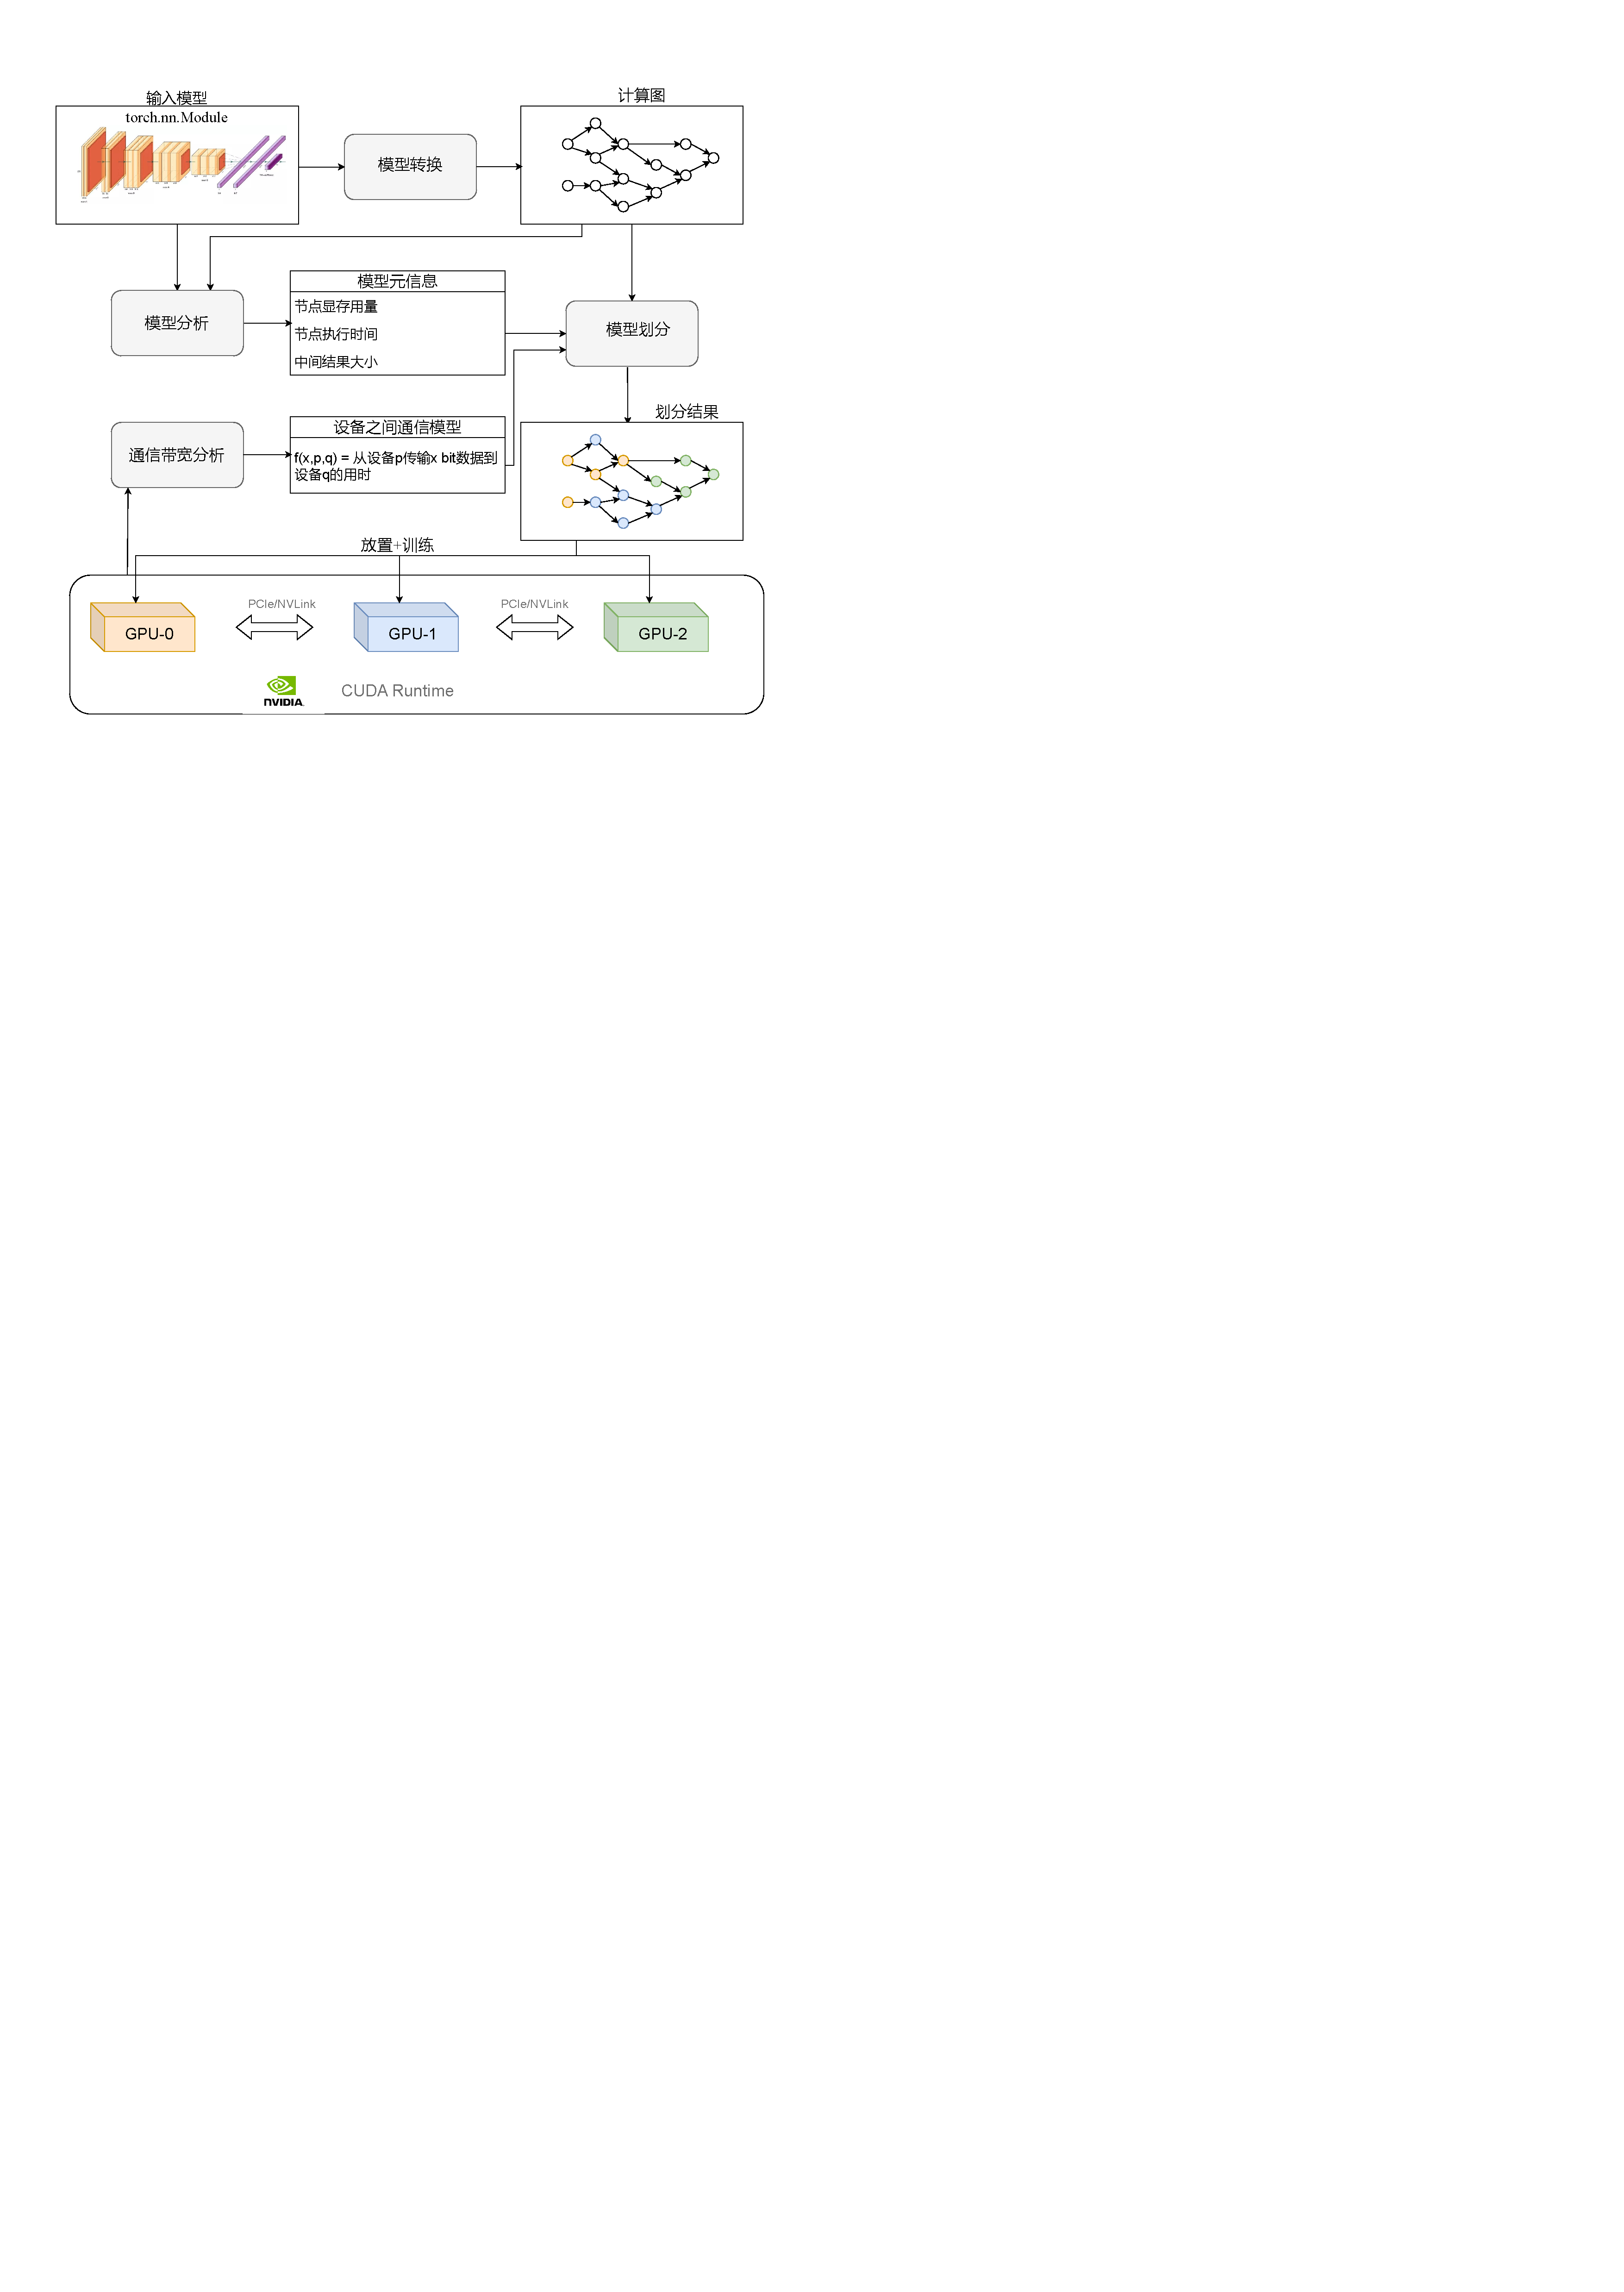
\includegraphics[width=0.95\textwidth]{figure/3-system/arch2.pdf}
	\caption{\sys{} 总体架构}
	\label{fig:arch}
\end{figure}

基于\ref{sec:analysis} 中对大型神经网络模型训练中的问题的分析,我们设计并实现了\sys{}。
\sys{} 是基于PyTorch的,针对大型神经网络进行自动化训练的框架。通过提供自动化的模型分析,硬件环境分析,模型转化,模型划分等功能,尽可能简化大模型等训练流程,减少人工参与,解决大模型难以训练的问题。
\sys{} 支持对通用的PyTorch模型进行训练,无需使用者对模型进行预处理。
\sys{}接受用户定义的模型作为输入,并自动完成模型结构理解,对模型进行转换,得到模型底层计算图的中间表示。然后通过动态分析和静态分析的方式,获得模型的元信息,包括计算图中节点的显存用量,计算图中节点的执行时间等。同时,\sys{} 采集参与训练的硬件的信息,并测试设备之间的点对点通信带宽。
然后模型划分模块接受模型元信息、模型计算图以及设备信息为输入,给出模型的划分结果。最后训练模块根据模型的划分结果进行模型到设备的放置,并启动训练流程,完成训练。
整体框架如图 \ref{fig:arch}所示,各个功能模块的简介如下:
\begin{itemize}
	\item \textbf{模型转换模块}: 负责进行模型结构的理解,实现用户输入的PyTorch模型和计算图中间表示的相互转换,从而允许框架对封装层次较高的模型进行进一步细分。
	\item \textbf{模型分析模块}: 通过动态分析和静态分析的方式,获取模型计算图中每个节点的前向传播/反向传播执行用时,计算图中每条边的传输的数据量,计算图中每个节点使用的内存。
	\item \textbf{通信测试模块}: 对参与训练的设备进行通信带宽的基准测试,来获取设备之间的点对点通信带宽,用于估算跨设备的通信时间。
	\item \textbf{模型划分模块}:模型划分模块是\sys{} 的核心模块,该模块根据模型分析模块和通信测试模块的输出,使用约束优化对模型计算图进行划分。
	\item \textbf{训练运行时模块}:划分好的模型由运行时模块放置到设备上进行训练,改模块根据计算图的划分结果重建模型,并处理节点之间的跨设备通信。
\end{itemize}

\section{本章小结}
本章首先分析了对大型神经网络模型进行训练的难点,例如大型神经网络模型参数量巨大,结构复杂,难以进行分析和预处理,另一方面参与训练的硬件设备也会影响训练的效率。
然后,介绍了对大型神经网络模型进行训练这一问题的分解,我们将问题分解为模型结构理解、模型元信息提取、训练环境分析和模型的划分与训练这四个子问题。
最后,本章介绍了基于PyTorch的\sys{}的设计。
\sys{}提供了对大型神经网络的自动化划分和训练功能,尽可能的简化了大型神经网络的训练流程。

下一章,我们将介绍\sys{}中各个功能模块的实现。
\chapter{大型神经网络训练框架的实现}
\label{chapter:implementation}
% 框架的整体结构,包含哪些模块
% 模块介绍
% 模型转换模块,model -> IR -> model
% 通信代价profiling
% 模型 profiling
% 模型内存代价预估
% 模型划分模块
% 训练模块

% 为了帮助研究者更方便的设计和实现神经网络模型,多种流行的神经网络框架被设计出来,并得到了广泛的使用,例如PyTorch, Tensorflow等。
% 但是目前的框架对于模型并行化训练的支持较为有限,仍然需要研究者手动对模型进行划分,手动管理模型和设备的映射关系。
% 针对当前框架的不足,我们基于PyTorch设计并实现了\sys{}。
% \sys{}提供了对大型神经网络的自动化划分和训练功能,尽可能的简化了大型神经网络的训练流程。
% 本章节首先介绍大型神经网络训练中的一些难点,然后介绍\sys{}的整体架构和各个功能模块。

在第三章中我们介绍了大型神经网络训练中的一些难点,对这些难点的分析,以及针对当前框架的不足,我们基于PyTorch设计的\sys{}。
本章我们将介绍\sys{}中的各个功能模块,包括进行模型结构理解的自动化模型转换模块(\ref{sec:convertion}),对设备之间的通信代价进行建模的通信代价建模模块(\ref{sec:commu}),进行模型显存代价分析(\ref{sec:mem})和计算代价分析(\ref{sec:time})的模型分析模块,以及对模型划分与训练模块(\ref{sec:partition-and-train})。

\section{自动化模型转换}
\label{sec:convertion}
% 1: 原始模型 - ONNX -> IR 
% 2: IR - fx.Graph -> 等价模型

\subsection{获取计算图}
在PyTorch中,通常使用继承了\texttt{torch.nn.Module}的类对模型进行描述,模型的计算图由\texttt{forward}函数隐式定义,在运行时由框架动态生成。
为了便于后续对模型进行划分,我们需要提取出隐式定义的计算图,将其转换为某种中间表示,例如由邻接表或者邻接矩阵所表示的图。

\begin{figure}[h]
	\centering
	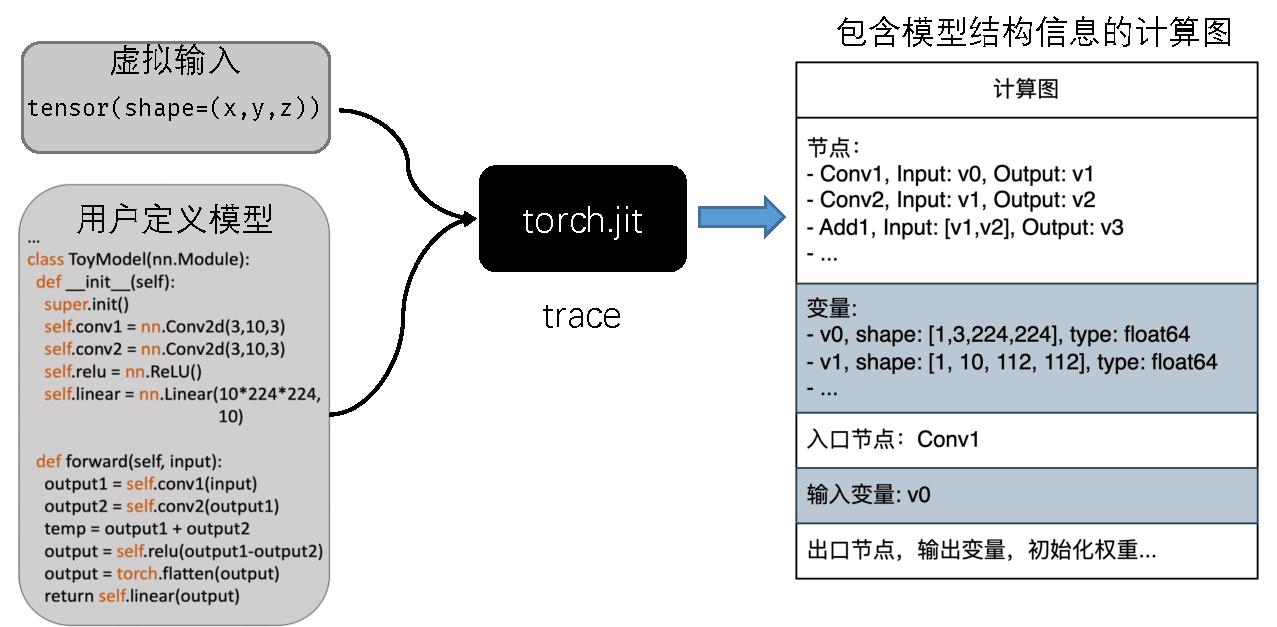
\includegraphics[width=0.9\textwidth]{figure/3-system/2ir.pdf}
	\caption{模型转换为中间表示}
	\label{fig:2IR}
\end{figure}

图 \ref{fig:2IR} 描述了从原始模型定义到中间表示的流程,首先框架将对模型进行即时编译和导出,将原始的PyTorch模型转换为通用的ONNX(Open Neural Network Exchange)格式\footnote[1]{https://github.com/onnx/onnx}的模型文件,然后框架读取模型文件,将其反序列化为计算图的中间表示。
其中,ONNX是一种通用的模型描述的格式。
作为一种较为通用的模型描述格式,ONNX内置了大量算子可以对应到不同框架的算子,表 \ref{table:onnx-operators}展示了部分ONNX算子和对应的PyTorch算子。

\begin{table}
	\centering
	\caption{ONNX与PyTorch的部分算子对应}
	\label{table:onnx-operators}
	\begin{tabularx}{\linewidth}{ p{2cm}  p{2.2cm}  p{5.8cm}  X  }
		\toprule
		\textbf{算子} & \textbf{输入} & \textbf{描述} & \textbf{对应PyTorch} \\
        \midrule
        Transpose & 
        input:tensor; perm:tuple; &
        根据perm对input的维度进行重新排列,功能类似于numpy中的np.permute
        & permute \\
        \midrule
        Flatten & 
        input:tensor; axis:int; &
        对输入张量input进行扁平化操作,输出output为2D矩阵。axis指定输出矩阵第一维的结束维度。
        例如输入张量的形状为$(a,b,c,d)$,axis=2,则输出矩阵的形状为$(ab, cd)$&
        flatten
        \\
        \midrule
        Upsample &
        input:tensor; scale:tensor;&
        对输入张量进行上采样,scale是一个长度等于input维数的张量,每一项指定了input的一个维度进行上采样时的缩放参数。例如对形状为$(a,b,c)$的输入张量进行上采样,scale=$(2,3,4)$,则输出张量的形状为$(2a,3b,4c)。$&
        interpolate
        \\
        \midrule
        Conv &
        input:tensor; w:tensor; bias:tensor; &
        使用w作为卷积核权重对输入张量input进行卷积运算,如果bias非空,则结果加上bias。&
        nn.Conv1d; nn.Conv2d; nn.Conv3d;
        \\
        \bottomrule
	\end{tabularx}
\end{table}

我们首先使用\texttt{torch.onnx.export} 对原始模型进行及时编译,追踪模型在运行过程中所使用的算子,得到等价的ScriptModule,然后将结果导出为ONNX格式的模型。
ONNX中定义了Graph,Node,Variable等结构体,解析ONNX文件,就可以得到模型的计算图的中间表示。
我们使用邻接表的形式描述计算图,在计算图中,如下字段会被存储:
\begin{itemize}
	\item Nodes: 记录计算图中所有的节点,每一项都是一个节点,代表一个算子。对于每个算子,我们记录它的类型,名称,输入变量和输出变量,注意有一些算子例如Add会有超过一个输入变量,因此输入变量和输出变量都使用集合进行存储。
	\item Variables: 记录图中的所有边,每一项都是一个边,代表一个变量。对于每个变量,我们记录它的数据类型,名称以及形状。后续我们可以根据数据类型和形状推断出变量使用的显存大小。
	\item EntryNodes:计算图的入口节点,可能不唯一。
	\item InputVariables: 计算图的输入变量,可能不唯一。
	\item OutputVariables: 计算图的输出变量,可能不唯一。
	\item Initializers: 对于某些特殊的算子,有可能需要为其提供初始权重,例如批归一化(BatchNormalization)层。
\end{itemize}

\subsection{模型重建}
除了从原始模型中提取出模型底层的计算图之外,自动化模型转换模块的另一个重要功能是从计算图中间表示重建出和原模型等价的PyTorch模型。
在原始的模型定义中,计算图的节点和边在\texttt{forward}函数中被隐式定义,这种隐式定义计算图的方式为后续的模型划分和放置带来了困难。
当我们在计算图中应用了模型的划分结果后,需要在计算图中添加额外的通信节点。例如计算图中存在边$\langle u,v\rangle$,节点$u$被划分到了设备-0上,节点$v$被划分到了设备-1上,那么必须在$u$和$v$之间添加额外的通信节点$w$,$w$负责从设备-0上接受变量,并将其放置到设备-1上。
也就是说原来的边$\langle u,v\rangle$会被$\langle u, w\rangle$ 和$\langle w,v\rangle$取代。

由于在原始模型中计算图是隐式定义的,因此上述对于计算图进行修改的操作难以在不修改\texttt{forward}函数本身的条件下实现。
为了更方便的修改计算图,我们的解决方案是从原始计算图中重建出和原模型等价的\texttt{torch.fx.GraphModule}。
\texttt{torch.fx} \upcite{torchfx} 工具包提供了对PyTorch模型进行变换以及构建PyTorch模型的功能。
与通过\texttt{forward}对计算图进行隐式定义的\texttt{nn.Module}实例不同,\texttt{GraphModule}通过直接定义计算图的方式构建模型。
具体的,一个\texttt{torch.fx.GraphModule}中包含了若干算子,以及一个用于描述这些算子之间计算依赖关系的\texttt{torch.fx.Graph}实例。
在\texttt{torch.fx.Graph}中,有一系列节点,每个节点除了记录对应的算子,还记录了参与运算的变量,通常参与运算的变量是其他节点的输出。

\begin{lstlisting}[language=Python, caption={模型重建}]
import torch.fx as fx 
torch_graph = fx.Graph() 
place_holders = {}
wrapper_module = nn.Module()
# nodes are already topo-sorted.
for ir_node in graph.nodes:
  node = convert_to_torch(ir_node)
  wrapper_module.add_module(node, name=ir_node.name)
  args = []
  for var in ir_node.inputs:
    if var.type == GRAPH_INPUT:
	  args.append(graph.inputs[var.id])
	elif var.type == GRAPH_INITIALIZER:
      args.append(graph.initializers[var.id])
	elif var.type == NODE_OUTPUT:
	  input_node_name = g.find_node_name(var)
	  input_node = place_holders[input_node_name]
	  args.append(input_node)
  place_holders[ir_node.name] = torch_graph.call_module(ir_node.name, args)
return fx.GraphModule(graph=torch.graph, root=wrapper_module)
\end{lstlisting}

在获取到计算图之后,我们可以根据计算图构建出等价的模型,上面的伪代码展示了构建的过程。
首先创建出记录计算图信息的\texttt{torch.fx.Graph}对象,以及用于存储计算图中节点对应的PyTorch算子的容器\texttt{wrapper\_module}。
然后按照拓扑排序的顺序对计算图中的节点进行遍历,对于每个中间节点\texttt{ir\_node},寻找它的输入变量,如果输入变量来自计算图,则直接使用变量名,如果输入变量来自其他节点的输出,则使用该节点作为输入。
所有输入变量确定后,用\texttt{placer\_holders}记录算子之间的计算关系。
图中所有节点遍历完成后,就得到了存储所有节点对应的PyTorch算子的容器\texttt{wrapper\_module},以及记载了这些算子之间计算关系的\texttt{torch\_graph},从\texttt{wrapper\_module}和\texttt{torch\_graph}就可以得到所需的\texttt{fx.GraphModule},并返回。

\section{通信代价建模}
\label{sec:commu}
% 为什么: 通信不可忽略; 通信链路异构
% 怎么做: 线性建模
分布式深度学习不仅是计算密集型任务,也是通信密集型任务。
在进行模型并行化训练时,模型被分散在不同的设备上,前向传播的中间结果和反向传播的梯度通过设备之间的通信在不同的算子之间传输。
而设备之间的通信时间不可忽略,图 \ref{fig:overhead} 展示了使用4张1080Ti GPU在CIFAR-10 \upcite{cifar}数据集上训练VGG19 \upcite{vgg}模型时,不同的步骤耗时的分解。
可以发现即使CIFAR-10是很小的数据集,通信时间也占据了总用时的40\%。

\begin{figure}[h]
	\centering
	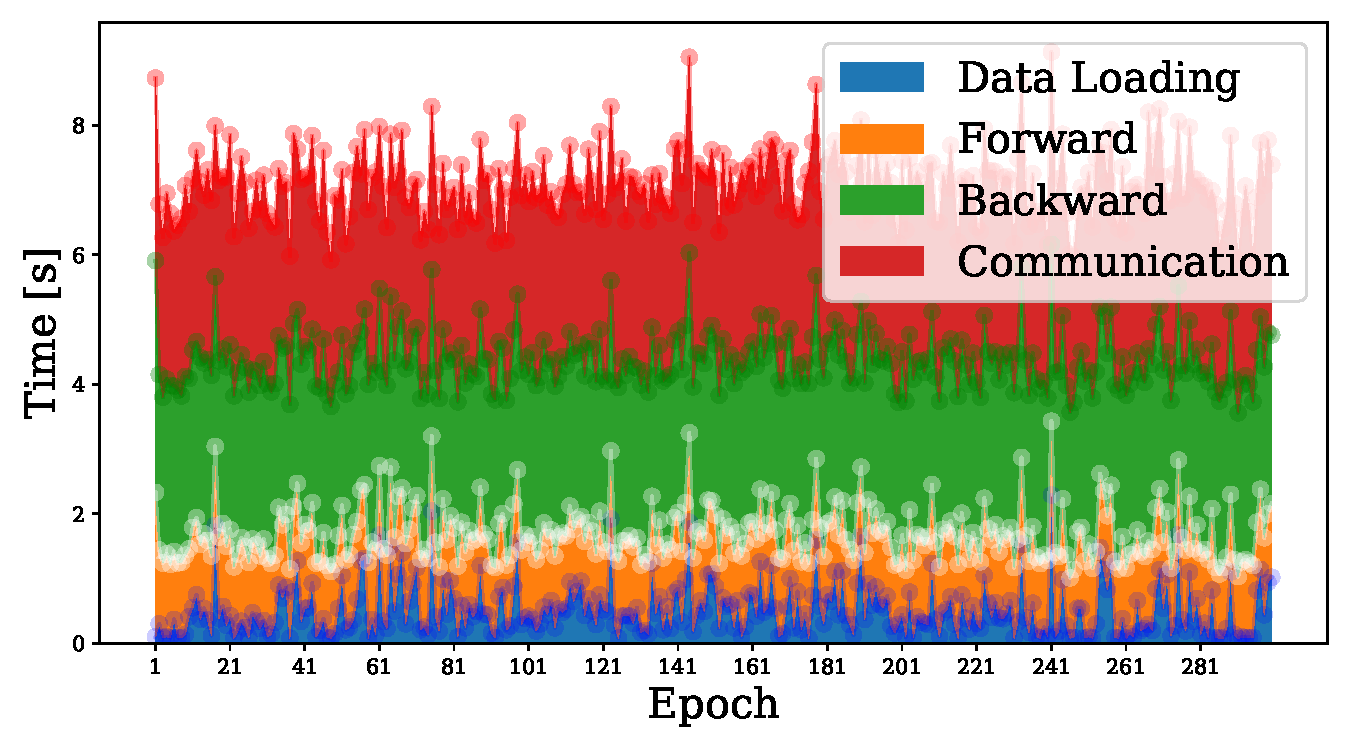
\includegraphics[width=0.85\textwidth]{figure/3-system/overhead_decomposition.pdf}
	\caption{训练用时分解}
	\label{fig:overhead}
\end{figure}

\begin{figure}[h]
	\centering
	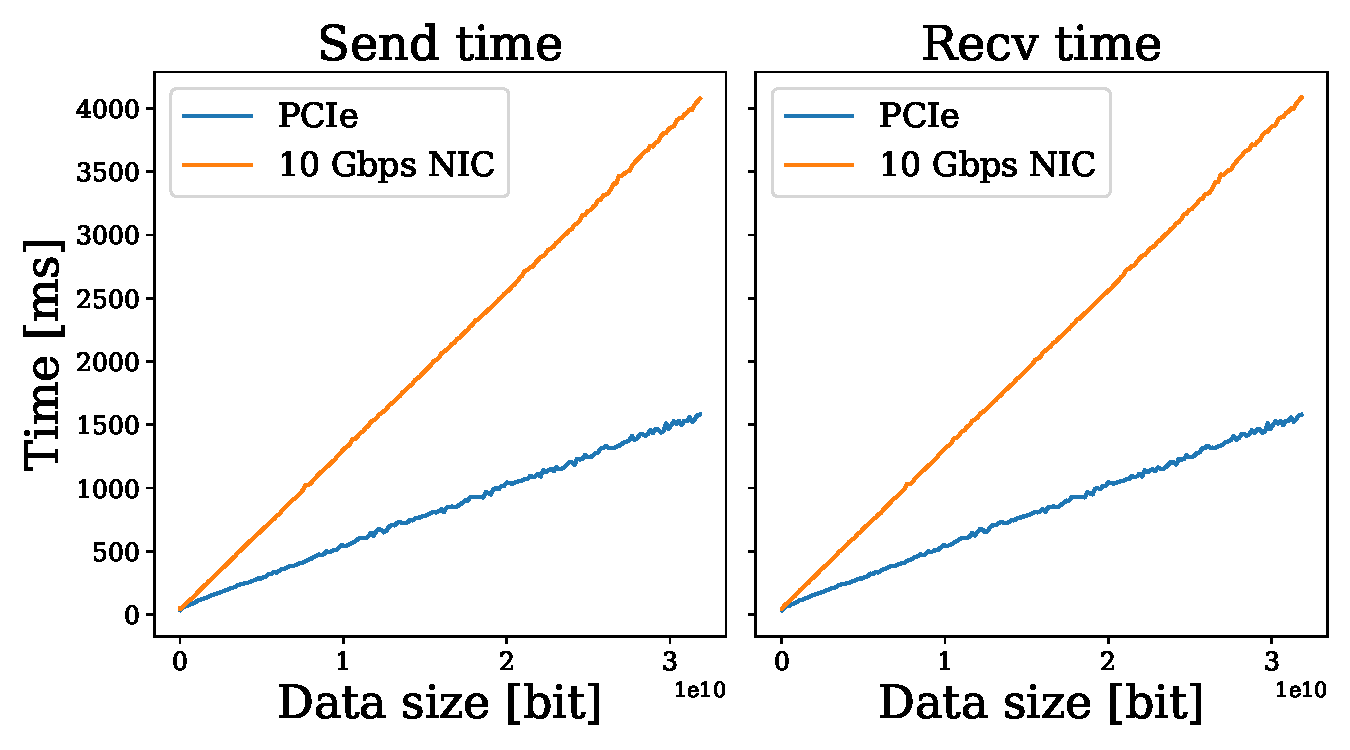
\includegraphics[width=0.85\textwidth]{figure/3-system/commu.pdf}
	\caption{通信用时和传输数据量的关系}
	\label{fig:linear}
\end{figure}
在神经网络模型中,节点与节点之间通信的数据量会随着节点类型变化而变化。
例如某个节点对应卷积操作时,输出数据的通道数目相比于输入数据会增加,因此输出数据的大小会增加,所需要的通信时间也更多。
而某个节点如果对应池化操作,输出数据可以看作是对输入数据进行下采样,因此输出数据的大小会减少,所需要的通信时间也更少。
因此在对模型进行划分时,我们需要考虑节点的输出数据的大小,通过合理的划分,让设备与设备之间传输的数据量更少,从而达到优化通信代价的效果。

另一方面,在优化通信代价时,除了需要考虑节点之间通信的数据量,也需要考虑设备与设备之间的通信链路。
在计算集群中,设备之间的通信链路往往是异构的。
例如设备可以通过高性能专用通信设备,如NVLink,NVSwitch通信,也可能通过通用的PCIe或者以太网进行通信。
因此在进行通信代价优化时,设备之间通信链路的异构性也需要被考虑。
我们设计了通信测试模块来对设备之间的点对点通信带宽进行建模。
图 \ref{fig:linear}展示了设备通过10Gbps的以太网卡和通过PCIe Switch进行通信时,传输的数据量和用时的关系,可以发现传输数据量和通信时间呈现出线性关系,因此我们使用线性模型对通信代价进行建模。
通信测试模块在设备之间发送不同大小的数据包,并记录数据包对应的传输时间,
然后对传输时间和数据大小两类数据进行线性拟合,获得通信时间的预测模型,在给定数据包大小的情况下,可以准确预测通信时间。
通信时间预测模型在后续的模型划分模块中用来预测给定的划分的通信代价,指导模型划分模块对通信代价进行优化。

\section{显存代价估计}
\label{sec:mem}
% 1. 模型: 参数 + 梯度 + 动量
% 2. 中间结果: 张量大小 + 梯度 + 动量 
模型并行化主要解决单个设备的显存容量有限,难以满足大模型训练时对于显存的需求。
设备的显存容量可以通过查看设备信息获得,而模型训练时所需要的显存对于开发者来说是未知的,当开发者进行手动模型划分时,难以保证划分后的模型在设备上训练时仍然满足设备的显存限制,因此我们需要一种可以预估模型显存占用的方法,用来判断某种模型划分是否可以满足当前硬件设备的限制。

\begin{table}
	\centering
	\caption{计算图的显存开销}
	\label{table:model-mem}
    \begin{tabularx}{\linewidth}{p{2.4cm} p{2.6cm} X }
        \toprule
        \textbf{种类} & \textbf{类型} & \textbf{描述} \\
        \midrule
        \multirow{2}*{节点} & 参数 & 算子中可以学习的参数,例如卷积中的卷积核 \\
        \cmidrule{2-3}
        & 参数梯度 & 在反向传播过程中计算出的用于更新参数的梯度,大小与对应参数大小相同,随着优化器的不同,可能还有动量与二阶动量 \\
        \midrule
        \multirow{4}*{边} & 模型输入 & 计算图的入口节点从数据加载器获得的输入数据批(data batch) \\
        \cmidrule{2-3}
        & 算子输入 & 计算图中算子的输入变量 \\
        \cmidrule{2-3}
        & 算子输出 & 计算图中算子的输出变量,对于该算子的后继算子来说,如果后继和该算子在同一个设备上,则该算子的输出变量等同于后继算子的输入变量 \\
        \cmidrule{2-3}
        & 变量梯度 & 在反向传播过程中计算出的变量梯度,用于计算参数梯度 \\
        \midrule
        固定开销 & CUDA上下文 & 包括CUDA运行时,cuDNN Lib加载等需要占用的显存 \\
        \bottomrule
    \end{tabularx}
\end{table}

由于我们在计算图的层面对模型进行划分,因此显存预估也在计算图的层面上进行。
计算图中,每个节点所对应的算子会消耗显存,每个边也会消耗显存,具体来说,我们可以将模型的显存占用分为以下的三部分:
\begin{itemize}
	\item 模型参数:模型参数也就是模型中需要进行学习和更新的张量,这部分显存消耗来自于计算图中的节点,每个节点对应的算子如果有需要进行学习的参数,都会占用一部分显存来存储这些参数。
	\item 中间结果:在计算图中,每个节点代表一个算子,而每条有向边就对应算子运算的结果。
	这些中间结果由前一个算子输出,并且作为后一个算子的输入。中间结果会被暂存,用来在反向传播时计算梯度。
	\item 梯度:在反向传播过程中,被计算得到用于更新模型参数。一般来说梯度所使用的显存大小等同于模型参数所使用的显存大小,对于某些优化器来说,除了需要计算梯度,还会存储动量(Momentum)以及二阶动量,因此会有额外的显存开销。
	总显存开销应该是模型参数所需的显存开销的整数倍。
\end{itemize}

表 \ref{table:model-mem} 详细的描述了模型训练中的几种显存开销,下面我们将介绍如何对这几种显存开销进行预估。
\begin{table}
	\centering
	\caption{几种算子模型参数显存开销}
	\label{table:operator-mem}
    \begin{tabularx}{\linewidth}{ p{2.4cm} p{3.8cm} X }
        \toprule
        \textbf{算子} & \textbf{参数大小} & \textbf{描述} \\
        \midrule
        Conv2D & $C_{in} \times C_{out} \times K_{h} \times K_{w}$ & 二维卷积算子的模型参数量等于卷积核的数目乘以每个卷积核的大小 \\
        \midrule
        Linear  & $F_{in} \times F_{out} + F_{out}$ & 线性变换算子的模型参数量等于线性变换矩阵大小加上偏置大小 \\
        \midrule
        BatchNorm2D & $2\times C $ & BatchNorm2D对输入执行批归一化,也就是计算$y=\frac{x-E(x)}{\sqrt{var(x)+\epsilon}} \times \gamma + \beta$,对于输入数据的每个通道,都需要存储相应的$\gamma$和$\beta$ \\
        \bottomrule
    \end{tabularx}
\end{table}

\begin{algorithm}[h]
	\caption{判定划分是否满足内存约束}
	\label{alg:estimate-mem}
	\begin{algorithmic}[1]
	\REQUIRE $\mathit{NodeToDevice}$, $\mathit{Nodes}$, $\mathit{MemCapacity}$
	\ENSURE  $\mathit{isValid}$
	\STATE   $\mathit{VariablesOn} \leftarrow \mathrm{Map}[\mathrm{int}, \mathrm{Set}]$
	\STATE   $\mathit{DeviceMem}_{0,1,\dots,n} \leftarrow 0$
	\FOR{ $\mathit{Node}\ n\ \in \mathit{Nodes}$ }
		\STATE $device \leftarrow \mathit{NodeToDevice}[n]$
		\FOR{$\mathit{Variable}\ input\ \in\ n.\mathit{inputs}$}
			\IF{$input \not\in \mathit{VariablesOn}[device]$}
				\STATE $\mathit{VariablesOn}[device].add(input)$
				\STATE $\mathit{DeviceMem}_{device}\ \leftarrow \ \mathit{DeviceMem}_{device} + input.size \times 2 $
			\ENDIF
		\ENDFOR
		\FOR{$\mathit{Variable}\ output\ \in\ n.\mathit{outputs}$}
			\IF{$output \not\in \mathit{VariablesOn}[device]$}
				\STATE $\mathit{VariablesOn}[device].add(output)$
				\STATE $\mathit{DeviceMem}_{device} \leftarrow  \mathit{DeviceMem}_{device} + output.size \times 2 $
			\ENDIF
		\ENDFOR
		\STATE $\mathit{DeviceMem}_{device} \leftarrow  \mathit{DeviceMem}_{device} + n.weight.size + n.gradient.size$
	\ENDFOR
	\STATE $\mathit{isValid}\leftarrow \mathrm{TRUE}$
	\FOR{$i:=0; i < n; i++$}
		\IF{$\mathit{DeviceMem}_{i} > \mathit{MemCapacity}_{i}$}
			\STATE $\mathit{isValid}\leftarrow \mathrm{FALSE}$
		\ENDIF
	\ENDFOR
	\RETURN $\mathit{isValid}$
	\end{algorithmic}
\end{algorithm}

\textbf{计算图节点开销}: 计算图节点的显存开销来自模型参数和训练过程中用于优化模型参数所产生的梯度以及可能的动量,二阶动量等。大部分节点所对应的算子,例如激活函数算子,二元运算算子等都没有可以学习的参数,因此这些算子的节点不会直接产生显存开销。表 \ref{table:operator-mem} 列举了部分会产生模型参数显存开销的算子,以及对应的开销的计算方法。
模型参数梯度与模型参数大小相同,因此显存开销相同。但是不同的优化器中,除了需要使用梯度,也会使用动量或者二阶动量来记录梯度下降的历史信息,控制梯度下降的优化方向。例如在Adam优化器 \upcite{adam}中,会用到动量和二阶动量,因此会产生为模型参数显存开销3倍的显存开销,用于存储梯度、动量和二阶动量。

\textbf{计算图边开销}: 计算图中,每个边都代表一个中间结果变量,存储这些变量和变量的梯度会带来显存开销。此外,如果边两端的节点在同一个设备上,那么边上的变量只会产生一次开销,而如果边两端的节点在不同的设备上,则边上的变量会分别作为节点输入和节点输出在两个设备上都产生显存开销。

\textbf{固定显存开销}: 固定显存开销主要来自加载模型训练所需的算法库,这部分开销相对固定,可以在启动任务前通过API得到。

在得到计算图中每个节点和每条边的显存开销后,我们就可以将其作为模型的元信息输入到模型划分模块中,来指导模型划分模块进行模型划分,避免划分后的模型过大,导致某个设备出现显存溢出的问题。
算法 \ref{alg:estimate-mem}展示了如何判定给定的模型划分是否可以满足内存约束。
算法的输入中,$\mathit{NodeToDevice}$ 是划分结果,是一个从节点到设备的映射。
$\mathit{Nodes}$ 是计算图中所有节点按照拓扑排序后得到的节点列表,列表中的每一项都是一个节点,记载了节点的输入变量,输出变量,每个变量的大小,以及节点的参数大小。
$\mathit{MemCapacity}$ 是设备的显存容量。
首先,算法中声明了临时变量$\mathit{VairablesOn}$,用来存储某个设备上已经存在的变量。
算法的最外层循环对节点列表进行遍历,对于每个节点,分别遍历它的输入变量,输出变量,如果变量不在节点所在的设备上,则将变量加入到当前设备上,并将变量使用的显存加到当前设备的显存用量$\mathit{DeviceMem}$中。
最后将节点的参数,梯度,动量的显存占用也加入到节点所在的设备上,判定设备上的显存申请是否大于设备的显存容量,并返回结果$\mathit{isValid}$。



\section{计算代价分析}
\label{sec:time}
% HOOK + Virtual Node for Edge + 代码展示
获取一个好的模型划分的前提是模型划分模块有足够的模型元信息来指导模型的划分,除了需要模型计算图中每个节点的显存用量,还需要每个计算节点的计算用时。
有了每个节点计算用时,就可以指导模型划分生成训练用时更短的划分方案。
因此我们设计了计算代价分析模块,用于获取计算图中每个节点在训练时的前向传播用时和反向传播用时。
为了便于表述,我们记$FP_{v}$表示节点$v$的前向传播用时,$BP_{v}$表示节点$v$的反向传播用时。

由于计算用时和多种因素有关,包括使用的CUDA版本,硬件性能,具体的算子底层实现等,因此我们难以通过静态的方式确定每个算子的用时,所以我们采用动态分析的方式对每个算子的计算用时进行采集。
\sys{}基于PyTorch实现,PyTorch提供了Hook机制,帮助开发者注册模型训练时关键事件的回调(Call Back)函数,比如某个算子前向传播开始的事件。下面是PyTorch中支持的4种回调函数的注册方法:
\begin{itemize}
	\item \texttt{torch.Tensor.register\_hook(func)}: 向某个张量注册回调函数,当和该张量相关的梯度被计算出时,回调函数被触发。回调函数接受旧的梯度作为输入,可以在回调函数中对梯度进行修改操作,返回修改后的梯度。常用于在张量进行更新前,对梯度进行修改。
	\item \texttt{torch.nn.Module.register\_forward\_pre\_hook(func)}: 向某个神经网络模块注册回调函数,该回调函数在模块执行\texttt{forward()}方法前被调用,回调函数接受前向传播的输入,返回修改后的输入。常用于在模块执行前向传播之前,对输入进行修改。
	\item \texttt{torch.nn.Module.register\_forward\_hook(func)}: 向某个神经网络模块注册回调函数,回调函数在模块执行\texttt{forward()}方法后被调用,用来获取和修改前向传播的输出。
	\item \texttt{torch.nn.Module.register\_backward\_hook(func)}: 向某个神经网络模块注册回调函数,在该模块完成反向传播计算出梯度后被调用,可以用来获取并修改梯度。
\end{itemize}

通过PyTorch的Hook机制,可以获取模型计算图中各个节点在训练过程中的关键事件,比如前向传播开始,前向传播结束等,记录这些关键事件发生的时刻,就可以计算得到每个节点前向传播和反向传播计算过程的用时。
需要注意的是,PyTorch并没有提供记录某个模块反向传播事件开始的事件的方法,因此我们需要对原有模型进行修改。

我们设计了\texttt{WrapModule}类,该类继承自\texttt{torch.nn.Module}。
该类中封装了一个计算图中的节点,而且可以根据需要,动态为该节点添加虚拟后继节点,通过捕捉虚拟后继节点的反向传播完成事件,就可以得到原始节点的反向传播开始事件,从而计算出原始节点的反向传播用时,以下的代码展示了\texttt{WrapModule}的实现。
如代码所示,当调用\texttt{profile}方法时,通过设置\texttt{enable}可以开启计算时间记录或者关闭计算时间记录,当计算时间记录开启时,会为\texttt{self.\_torch\_module}添加虚拟后继节点,计算时间记录关闭时,则会移除该虚拟后继节点。

\begin{lstlisting}[language=Python, caption={WrapModule实现}]	
class VirtualModule(nn.Module):
	def forward(self, x, *args):
		return (x, ) + args if args else x
class WrapModule(nn.Module):
	def __init__(self, torch_module: nn.Module, node_name: str):
		super().__init__()
		self._torch_module = torch_module
		self._wrapped_module = torch_module
		self._virtual_successor = VirtualModule()

	def forward(self, *args, **kwargs):
		return self._wrapped_module(*args, **kwargs)
	
	def profile(self, enable:bool=True):
		if enable:
			# 开启计算时间记录
			self._wrapped_module = Sequential(self._torch_module, self.virtual_sucessir)
			...
		else:
			# 关闭计算时间记录
			self._wrapped_module = self._torch_module
			...
\end{lstlisting}

\begin{figure}[h]
	\centering
	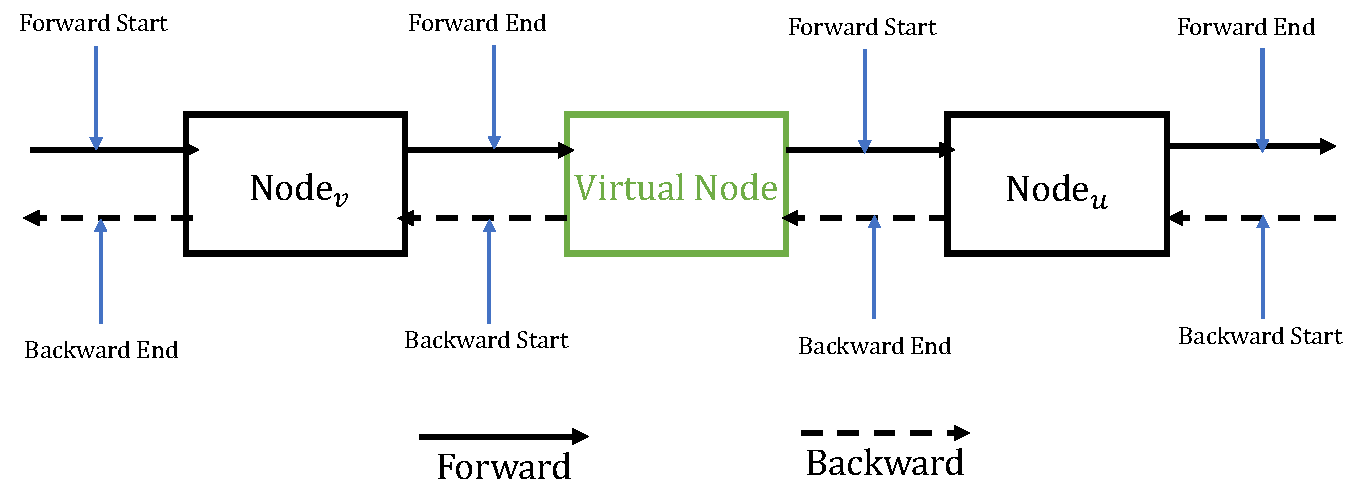
\includegraphics[width=0.8\textwidth]{figure/3-system/profile.pdf}
	\caption{计算代价分析}
	\label{fig:profile}
\end{figure}

在计算时间记录开启时,除了添加虚拟后继节点之外,还会注册回调函数函数,我们会记录节点的前向传播开始,前向传播结束,反向传播结束和虚拟后继节点的反向传播开始这四个事件的发生的时间,并计算得到节点的前向传播用时和反向传播用时,图 \ref{fig:profile} 展示了这一过程。
在实际实现中,我们首先使用Beachi \upcite{baechi}中的m-TOPO(带有内存约束的拓扑排序)划分方法对模型进行划分,这种划分方法具有内存约束,而且运行速度快,因此我们选择这种方法。
然后我们将初步划分好的模型放置到设备上,开启计算时间记录,并使用小批量数据进行训练,多次记录每个节点的前向传播和反向传播用时,并通过取平均值的方式减小误差,最后得到每个节点在当前硬件环境下的前向传播和反向传播用时。

\section{模型划分与训练}
\label{sec:partition-and-train}
% 输入, 输出
% Partitioner和Placer的设计
% 训练
在进行完通信代价建模,显存代价估计和计算代价分析三个步骤后,模型划分模块接受模型计算图以及上述三个步骤到输出,进行模型划分以及后续的模型训练。
\begin{figure}[h]
	\centering
	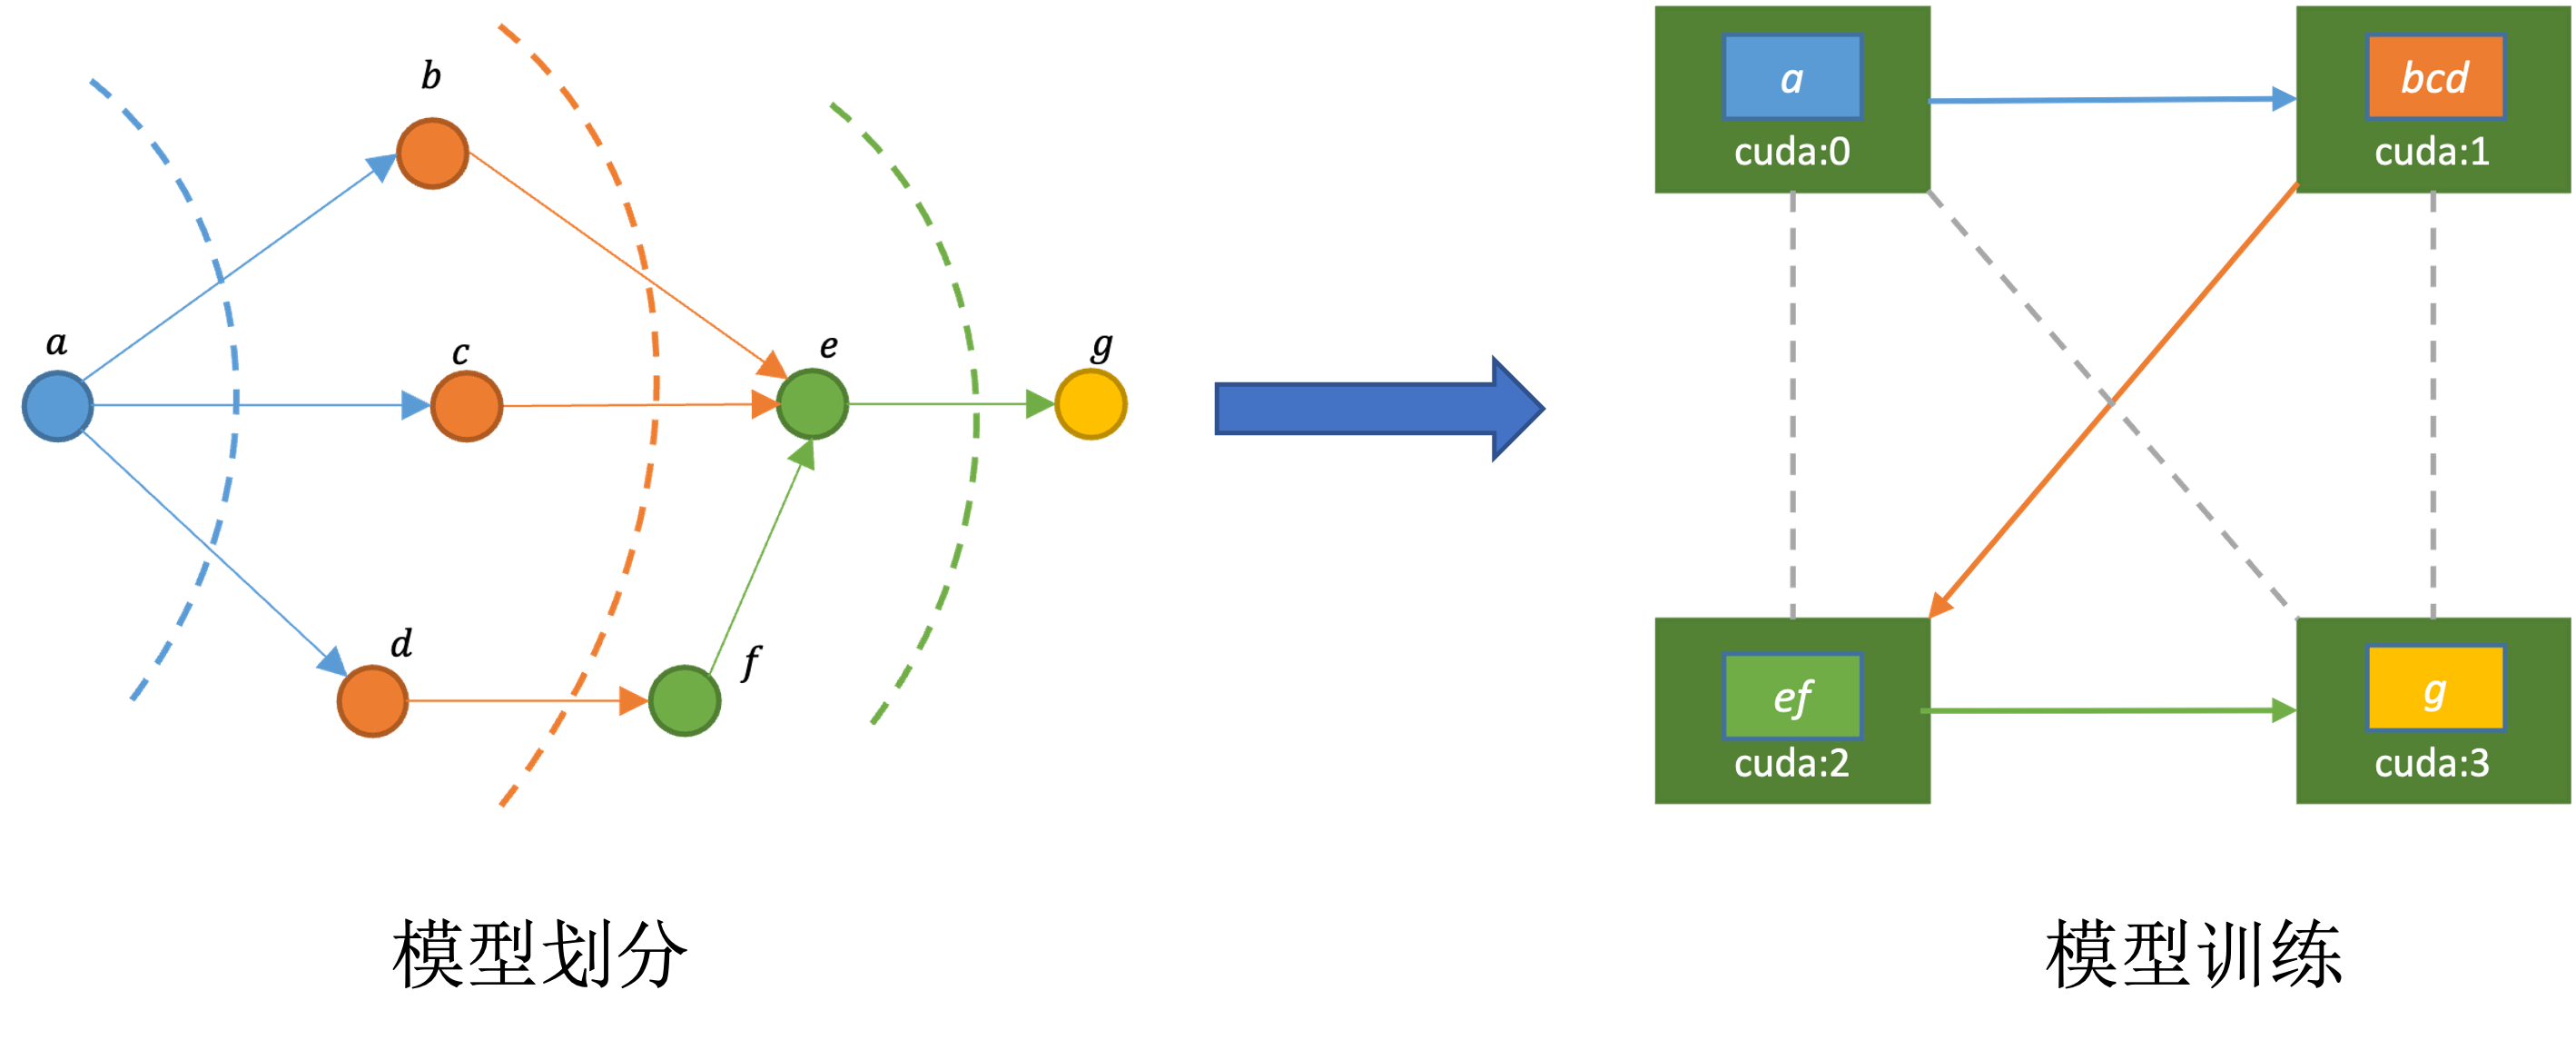
\includegraphics[width=0.9\textwidth]{./figure/3-system/partition_train.png}
	\caption{模型划分与训练}
	\label{fig:partition-and-train}
\end{figure}

图 \ref{fig:partition-and-train} 展示了模型的划分和训练。
模型划分模块为计算图中的节点寻找到设备的映射,在进行划分时,需要考虑设备内存约束,设备之间的通信带宽以及每个节点的计算代价,以最优化训练效率进行划分。
模型划分结束后,我们得到了划分结果,也就是节点到设备的映射。
然后模型训练模块会根据划分结果将模型放置到设备上,并启动训练流程。

在后续的实验中,我们会对比多种模型划分方法的效果,因此我们设计了\texttt{Partitioner}类作为所有模型划分方法的抽象基类。
\texttt{Partitioner}中只有一个\texttt{partition}一个方法,它的输入包括模型的计算图表示,设备信息,每个节点的计算用时信息,每个节点的显存使用信息以及设备之间的通信带宽。
获取输入信息后,\texttt{partition}运行特定的划分算法,给出划分结果,也就是节点到设备的映射。
不同的模型划分方法都需要继承自\texttt{Partitioner}类,并且实现\texttt{partition}方法。
具体划分算法的实现我们将在下一章进行介绍。

\begin{figure}[h]
	\centering
	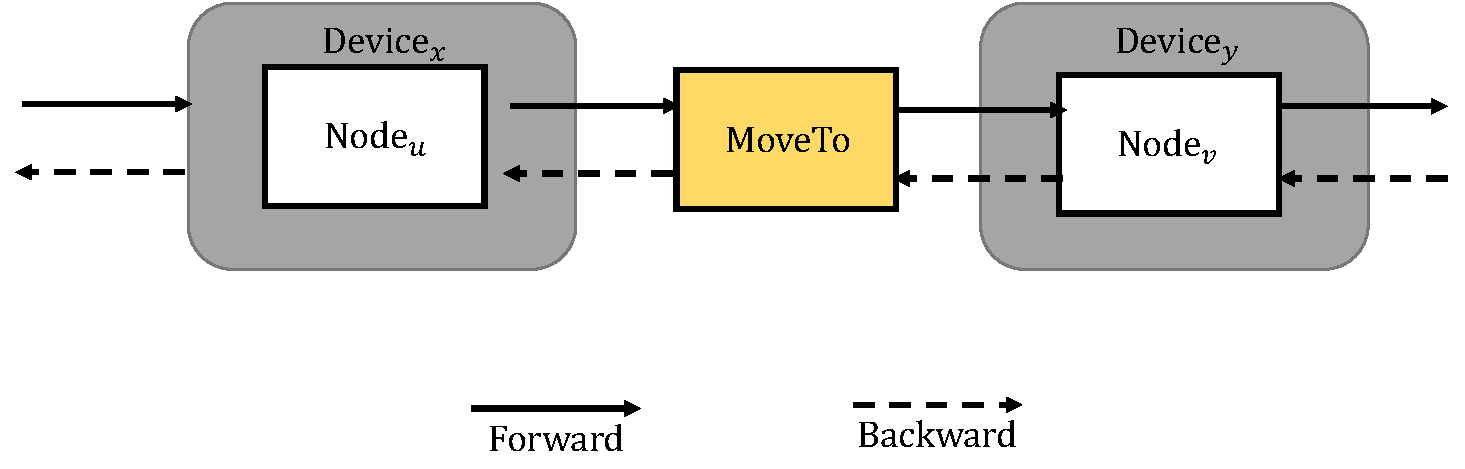
\includegraphics[width=0.9\textwidth]{./figure/3-system/moveTo.pdf}
	\caption{跨设备变量转移}
	\label{fig:move}
\end{figure}

\begin{algorithm}[h]
	\caption{添加变量转移节点}
	\label{alg:add-move}
	\begin{algorithmic}[1]
	\REQUIRE $\mathit{NodeToDevice}$, $\mathit{Nodes}$, $\mathit{Edges}$
	\ENSURE $\mathit{NewNodes}, \mathit{NewEdges}$
	\STATE  $\mathit{NewNodes} \leftarrow \mathrm{Set}[\mathit{Node}]$
	\STATE  $\mathit{NewEdges} \leftarrow \mathrm{Set}[\mathit{Edge}]$
	\STATE  $\mathit{CriticalEdges} \ leftarrow \mathrm{Set}[\mathit{Edge}]$
	\FOR{$\mathit{Edge}\ e \in \mathit{Edges}$}
		\STATE $\mathit{device}_u \leftarrow \mathit{NodeToDevice}[e.u]$
		\STATE $\mathit{device}_v \leftarrow \mathit{NodeToDevice}[e.v]$
		\IF{$\mathit{device}_u \neq \mathit{device}_v$}
			\STATE $\mathit{CriticalEdges}.add(e)$
		\ENDIF
	\ENDFOR
	\FOR{$\mathit{Edge}\ e \in \mathit{Edges}$}
		\IF{$e \in \mathit{CriticalEdges}$}
			\STATE $w \leftarrow \mathrm{NewMoveNode}(\mathrm{from}:\mathit{device}_u, \mathrm{to}:\mathit{device}_v)$
			\STATE $\mathit{NewEdges}.add(\left\langle e.u,w\right\rangle)$
			\STATE $\mathit{NewEdges}.add(\left\langle w,e.v\right\rangle)$
			\STATE $\mathit{NewNodes}.add(e.u,e.v,w)$
		\ELSE
			\STATE $\mathit{NewEdges}.add(e)$
			\STATE $\mathit{NewNodes}.add(e.u, e.v)$
		\ENDIF
	\ENDFOR
	\RETURN $\mathit{NewNodes}, \mathit{NewEdges}$
	\end{algorithmic}
\end{algorithm}

当得到划分结果后,我们还需要根据划分结果对模型再一次进行修改,显式的为跨设备的边添加变量转移节点。
如图 \ref{fig:move} 所示,计算图中有边$\langle u,v\rangle$,节点$u$被划分到了设备$x$上,节点$v$被划分到了设备$y$上,那么节点$u$的输出变量$u_{out}$默认会被放置在设备$x$上,
当节点$v$尝试去直接读取$u_{out}$时,会触发DeviceMismatch的错误,因此我们需要显式的在$\langle u,v\rangle$上添加将$u_{out}$放置到设备$y$上的变量转移节点。
变量转移节点本身不会带来新的计算代价,可以将变量转移节点看作是通信代价的一种表示,变量转移的过程实际上就是通信的过程。
变量转移节点也是通过继承PyTorch中的\texttt{nn.Module}类实现,在\texttt{forward}函数中,将输入变量放置到指定设备上并传递给后继计算节点去使用。

算法 \ref{alg:add-move} 展示了在计算图中添加变量转移节点的过程。首先我们在计算图中对边进行遍历,寻找所有两端点$u,v$不在相同设备上的边。
对于这种跨越不同设备的边,进行变量转移节点$w$的添加。
变量转移节点$w$会被添加到新的节点集合中,新生成的两条边$\left\langle u,w\right\rangle$ 和 $\left\langle w,v\right\rangle $也会被添加到新的边集。
最后返回新的节点集合和边集,由模型转换模块根据计算图重建模型,进行训练。



\section{本章小结}
本章介绍了\sys{}的设计和每个模块的具体功能。
对于如何实现模型和中间表示之间的相互转换,\sys{}提供了模型转换模块,可以完成用户定义的高层模型和计算图之间的相互转换。
对于模型分析,\sys{}提供了显存代价估计方法和计算代价分析方法,能够得到计算图中节点的显存占用和计算时间,指导模型的划分。
针对计算集群中存在的通信链路的异构性,我们设计了通信代价建模模块,可以对设备之间点对点通信链路进行带宽测试,从而建模通信代价。
获取节点显存占用,节点计算时间和设备通信建模后,\sys{}中的模型划分模块会进行设备划分,模型被划分到多个设备上进行训练。

本章主要介绍\sys{}中功能模块的设计与实现,下一章讲详细介绍模型划分模块中的算法的设计与实现。
\chapter{模型自动化划分方法设计与实现}
在第四章中,我们介绍了\sys{} 中的各个模块的作用,分别介绍了能够将原始模型转化为计算图中间表示的模型转换模块(\ref{sec:convertion}),能够得到设备之间通信带宽模型的通信代价建模模块(\ref{sec:commu}),能够对计算图中每个节点显存用量进行估计的显存代价估计模块(\ref{sec:mem})以及能够得到计算图中每个节点的前向传播和反向传播的时间的计算代价分析模块(\ref{sec:time})。这四个模块旨在为最关键的模型划分模块提供必需的信息,用于进行模型划分。在进行模型划分时,从计算图的层面上,模型划分模块生成从节点到设备的映射,本章将重点介绍\sys{}中使用的模型自动化划分方法。

% 问题形式化定义
% 图优化算法
% 图划分算法
\section{模型划分的形式化定义}
\label{sec:formul}
% 1. 符号表示约定
首先我们对模型划分的问题进行形式化定义,模型的划分也就是计算图的划分。
计算图是有向无环图(Directed Acyclic Graph, DAG),在计算图中,每个节点都表示一个计算过程,每条边都表示一个依赖关系,边的终点依赖与边的起点,所以要求计算图中不能有环,也就是从一个节点出发的路径不能再回到该节点,无环的特性保证了不会出现环形依赖,确保计算过程可以正确进行。

一个计算图可以由$\mathcal{G}=\langle \mathcal{V}, \mathcal{E}, \mathcal{V}_{\mathit{in}}, \mathcal{V}_{\mathit{out}} \rangle $四元组表示,除了节点集$\mathcal{V}$ 和边集$\mathcal{E}$ 之外,还有用于表示计算图入口节点的$\mathcal{V}_\mathit{in}$ 和计算图出口节点的 $\mathcal{V}_{\mathit{out}}$。
$\mathcal{V}_{\mathit{in}}$是入度为0的节点的集合,对应到神经网络模型中,就是读入训练数据的节点。
$\mathcal{V}_{\mathit{out}}$ 是出度为0的节点的结合,对应到神经网络模型中就是输出预测结果的节点。
图 \ref{fig:graph-example} 展示了一个典型的计算图,其中$\mathcal{V}_\mathit{in}$和$\mathcal{V}_\mathit{out}$中的节点被标记为红色。

\begin{figure}[h]
	\centering
	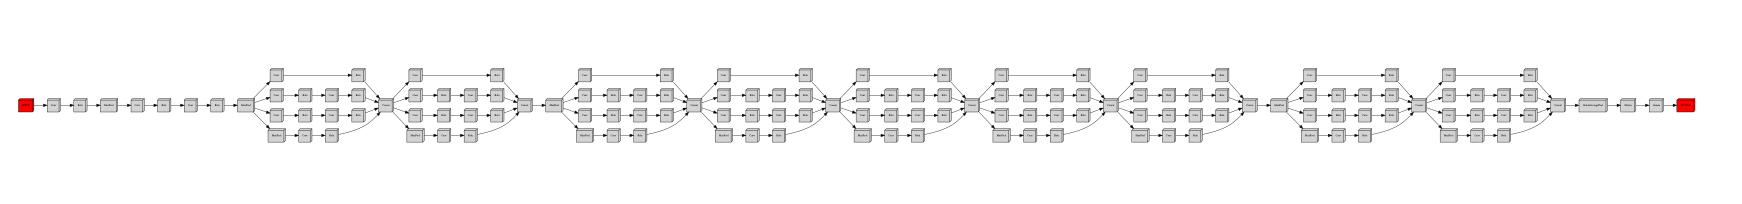
\includegraphics[width=\textwidth]{figure/4-alg/googlenet.png}
	\caption{GoogLeNet\upcite{googlenet} 的计算图}
	\label{fig:graph-example}
\end{figure}

\begin{table}[h]
	\centering
	\caption{模型划分模块的输入}
	\label{table:symbol}
    \begin{tabularx}{\linewidth}{p{3cm} p{3.2cm} X }
        \toprule
        \textbf{输出模块} & \textbf{符号表示} & \textbf{描述} \\
        \midrule
        \multirow{2}*{显存估计} & $\mathit{weight}_u$ & 节点$u$的参数所使用的显存,其中$u\in V$ \\
        \cmidrule{2-3}
        & $\mathit{size}_t$ & 中间变量$t$所使用的内存,通常来说,$t$对应$\mathcal{G}$中的某一条边,但是也有可能一个变量对应多个边,例如一个节点的输出变量可能是多个节点的输入边量。\\
        \midrule
        \multirow{2}*{计算代价分析} & $\mathit{FP}_{u}$ & 计算图中节点$u$的进行前向传播的计算用时,$u\in V$\\
        \cmidrule{2-3}
        & $\mathit{BP}_{u}$ &  计算图中节点$u$的进行反向传播的计算用时,$u\in V$\\
        \midrule
        通信建模 & $\mathit{Commu}(x,p,q)$ & 表示设备$p$和设备$q$之间传输数据量$x$的通信用时,如果$p=q$,则通信代价可以忽略不计。$Commu$就是设备之间的通信代价模型。 \\
        \bottomrule
    \end{tabularx}
\end{table}

$\mathcal{G}=\langle \mathcal{V}, \mathcal{E}, \mathcal{V}_{\mathit{in}}, \mathcal{V}_{\mathit{out}} \rangle $ 四元组由模型转换模块生成,并作为模型划分模块的一个输入,除了$\mathcal{G}$之外,模型划分模块还接受来自其他模块的输入,表 \ref{table:symbol} 中列举了除$\mathcal{G}$ 之外,模型划分模块接受的其他输入,以及这些输入的符号表示。
其中$\mathit{Commu}$是设备之间的通信代价模型。
对于每一对设备$p, q$,通信建模模块采集若干次设备之间点对点通信用时,通过线性拟合的方式构建设备之间的通信代价模型,模型接受通信数据量$x$,返回通信用时。

% 2. 问题的形式化定义
我们用$D$表示所有设备的集合,那么进行模型划分可以被看作寻找映射:$f: \mathcal{V}\mapsto D$,即为每个节点分配一个设备。
模型划分结果应该尽可能提升整个训练流程的数据吞吐量(Data Throughput)。
数据吞吐量表示了一个系统处理数据的速度,通常表示为单位时间内系统处理的数据量,当处理的数据量很大时,提高数据吞吐量就十分有必要。
在深度神经网络的训练中,数据吞吐量通常指单位时间训练完成的样本的数目,比如在视觉任务中,可以是每秒钟训练的图片数目,在自然语言处理任务中,可以是每秒钟训练的词向量数目。
提升数据吞吐量可以直接提升训练速度,缩短训练时间,因此模型划分模块以提升数据吞吐量为目标进行模型划分。
式 \ref{eq:target}描述了模型划分的目标,即在给定的硬件和计算图时,寻找可以使数据吞吐量(式中由$\mathcal{F}_{\mathit{throughput}}$表示)最大的划分,并满足显存约束。
\begin{equation}
	\label{eq:target}
	\begin{aligned}
		& \argmax_{f:\mathcal{V}\mapsto D} & \mathcal{F}_{\mathit{throughput}}(\mathcal{G}, D, f:\mathcal{V}\mapsto D) \\
		& \mathrm{s.t.} &\mathit{Memory}\ \mathit{Constraints}
	\end{aligned}
\end{equation}

\begin{equation}
	\label{eq:target2}
	\begin{aligned}
		& \argmin_{f:\mathcal{V}\mapsto D} & \mathcal{F}_{\mathit{iteration}}(\mathcal{G}, D, f:\mathcal{V}\mapsto D) \\
		& \mathrm{s.t.} &\mathit{Memory}\ \mathit{Constraints}
	\end{aligned}
\end{equation}

模型的训练具有迭代式的特性,每一轮迭代中模型对相同大小的数据批进行前向传播,通过损失函数计算损失,并且进行反向传播和参数优化。
每一轮迭代所需用时基本相同,因此最大化数据吞吐量等价于最小化单次迭代处理时间(Time Per Iteration )。
所以,式\ref{eq:target}也等价于式\ref{eq:target2},即寻找能最小换单次迭代用时的模型划分,其中单次迭代时间由$\mathcal{F}_{\mathit{iteration}}$表示。

\begin{figure}[h]
	\centering
	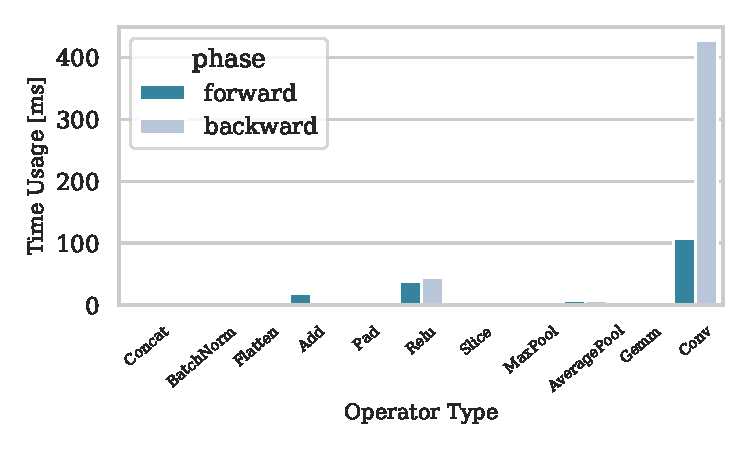
\includegraphics[width=0.85\textwidth]{./figure/4-alg/fp_bp.pdf}
	\caption{前向传播(FP)用时和反向传播(BP)用时的对比}
	\label{fig:fp-vs-bp}
\end{figure}

单次迭代时间是训练过程中,模型处理一个数据批的用时,包括前向传播和反向传播用时。
而现有的一些工作中,如Pesto \upcite{pesto} 中,简单的将单次迭代处理时间等价于计算图的执行用时,也就是训练过程中前向传播的用时,而忽略了反向传播的用时。
反向传播的代价不应该被忽略,图 \ref{fig:fp-vs-bp} 展示了在Amoebanet-D网络中,不同类型的算子的前向传播用时之和和反向传播用时之和。
可以发现,对于模型中的主要计算负载,二维卷积算子(Conv2D)的反向传播用时远远大于前向传播用时,因此在计算单次迭代用时时,算子反向传播的用时不能忽略。


\section{基于约束优化的模型划分}
\label{sec:algorithm}
% 简单介绍各个方向,然后说约束优化是主流
模型划分问题可以看作是带有通信依赖的任务调度问题在深度学习训练中的一种体现。
可以将计算图中的各个节点看作是一些有依赖关系的任务,将设备看作是一系列可以运行任务的处理器。
任务之间的依赖关系通过通信定义,如果任务B依赖任务A,则任务B需要通过通信获取任务A的输出,作为自己的输入。
被调度在相同处理器上的任务之间的通信时间可以忽略。
带有通信依赖的调度问题已经被证明是NP-Hard问题 \upcite{sched},因此无法在多项式时间内求出最优解。

现有工作 \upcite{rl1,rl2,baechi} 使用强化学习方法和近似算法进行模型划分,但是强化学习方法需要进行多次尝试和长时间的训练才能收敛。
而近似算法的使用场景较为有限,仅在通信计算比(Communication Computation Ratio, CCR)接近1时具有较好的近似比,而对于结构比较复杂的模型,由于计算图中边的数目较多,因此通信代价更大,CCR更大,所以近似算法难以获得较好的划分。
Hafeez等提出了Pesto\upcite{pesto},引入了约束优化方法进行模型划分。
本节接下来会首先会简单介绍Pesto中的约束优化算法以及其不足之处(\ref{sec:pesto}),然后详细介绍\sys{}中使用的约束优化算法(\ref{sec:core})和\sys{}中用来减少问题规模的节点协同放置算法(\ref{sec:co-place}),最后介绍\sys{}中的约束优化问题求解的实现(\ref{sec:picos-implement})。


\subsection{Pesto的约束优化}
\label{sec:pesto}
式\ref{eq:p-target} 到式\ref{eq:pst7} 给出了Pesto中对于模型划分约束优化的定义。
在Pesto中,假设原始的计算图表示为$\mathcal{G}=\left\langle \mathcal{E}, \mathcal{V}, \mathcal{V}_{in}, \mathcal{V}_{out}\right\rangle $。Pesto会预先对计算图进行修改,对于图中的每一个有向边$e=\left\langle i,j \right\rangle\in\mathcal{E}$,Pesto都会添加一个新的节点$k$,来表示节点$i$和节点$j$之间的通信,同时会用边$\left\langle i,k\right\rangle $和边$\left\langle k,j\right\rangle $替换边$\left\langle i,j\right\rangle $。
这样被修改后的图被表示为$\mathcal{G}=\left\langle \mathcal{\overline{E}},\mathcal{\overline{V}},\mathcal{\overline{V}}_{in},\mathcal{\overline{V}}_{out} \right\rangle$。
表示通信的节点的集合被记为$\mathcal{O}_{GG}$。


% Pesto的约束
\begin{align}
	& \mathrm{min} & &\mathcal{C}_{\mathit{max}} \label{eq:p-target}\\
	& \mathrm{s.t.} & &\mathcal{C}_i \le \mathcal{S}_j \quad \left\langle i,j \right\rangle\in \mathcal{\overline{E}}  \label{eq:pst1}\\
	& & &\mathcal{S}_i + p_i = \mathcal{C}_i  \quad\forall i\in \{\overline{\mathcal{V}} / \mathcal{O}_{GG} \}  \label{eq:pst2}\\
	& & &0\le \mathcal{C}_i\le \mathcal{C}_{\mathit{max}} \quad\forall i\in \overline{\mathcal{V}} \label{eq:pst3}\\
	& & & z_k = x_i \otimes x_j \quad\forall k \in \mathcal{O}_{GG}, (i,k),(k,j)\in\overline{\mathcal{E}} \label{eq:pst4}\\
	& & & S_i + z_i p_i = C_i \quad \forall i \in \mathcal{O}_{GG}\label{eq:pst5} \\
	& & & x_i \in \{0,1\} \quad\forall i \in \mathcal{O}_{GG} \label{eq:pst6}\\
	& & & \text{Memory Constraints and other constraints.} \label{eq:pst7}
\end{align}

在Pesto的约束优化问题的定义中,式\ref{eq:p-target}给出了约束优化要优化的目标,即最大完成时间。
约束\ref{eq:pst1} 表示对于计算图中的每条边$\left\langle i,j\right\rangle $,都有节点$j$的开始时间大于等于节点$i$的完成时间,即表达了各个节点之间的依赖关系。
约束\ref{eq:pst2} 表示对于每个非通信节点$i$,都有结束时间$\mathcal{C}_i$等于开始时间$\mathcal{S}_i$加上该节点的计算用时$p_i$。
约束\ref{eq:pst3} 定义了优化目标$\mathcal{C}_{max}$的下限,即整个计算图的执行时间应该在所有节点执行完成后。
约束\ref{eq:pst4} 定义一组指示随机变量(Indicator Variables) $z_k$,对于$\mathcal{O}_{GG}$中的节点$k$,如果它两端的节点$i$和$j$在同一个设备上,即$x_i=x_j$,则$z_k=0$,否则$z_k=1$。
对于通信节点$i$,约束\ref{eq:pst5}会根据$z_i$的值计算通信结束的时间,如果参与通信的两个节点在同一个设备上,则通信用时可以忽略,因此有$\mathcal{C}_i=\mathcal{S}_i$,否则需要考虑通信用时$p_i$。
Pesto的约束只适用于设备数目为2的场景,因此在约束\ref{eq:pst5}中,用于指示节点$i$最终被划分到哪个设备的变量$x_i$的取值是0或者1,但是在多个设备的情况下,需要进行扩展。
最后,Pesto加入了内存约束以及其他有关通信的约束。

尽管Pesto给出了用约束优化进行模型划分的思路,但是从Pesto给出的约束优化问题的定义来看,仍然有一些不足之处:
\begin{itemize}
	\item Pesto只考虑了设备数目为2的情况:在设备数目为2时,可以通过简单的异或运算确定两个节点是否在同一台设备上,但是需要扩展到多个设备的场景时,需要更复杂的约束条件。无法只通过一个二元变量来简单的表达节点被划分到哪个设备上。
	\item Pesto没有考虑通信的异构性:对于设备数目为2的情况,由于设备之间只有一条通信链路,因此可以简单的通过$p_i$来表示通信过程$i$的用时,但是在真实场景中,当设备数目大于2时,设备之间通常有多条通信链路,这些通信链路往往是异构的,通信过程$i$发生在不同的通信链路上可能对应不同的通信用时,Pesto的约束条件并没有加入对与通信异构性的考虑。
	\item Pesto没有考虑反向传播:在Pesto的约束中,最小化的目标是计算图的执行时间,也就是所有节点完成前向传播的时间。在训练过程中,单次迭代用时由前向传播和反向传播两部分的用时构成,而反向传播的用时无法忽略,因此只有在优化目标和约束中加入有关反向传播的部分才可以更准确的指导模型的划分。
	\item 缺少显存约束的详细表达:每个设备上的节点和变量使用的显存数目不能超过当前设备的最大容量,而Pesto没有给出显存约束的详细表达。
\end{itemize}

\subsection{\sys{}的约束优化}
\label{sec:core}
\begin{align}
	& \text{min} & & \mathit{Makespan} \label{eq:op-target} & \\
	& \text{s.t.} & & \mathcal{S}_{fp,i}=0 &\Gamma^{-}(i)=0, i\in \mathcal{V} \label{eq:cons1}\\
	& & & \mathcal{S}_{bp,i}=\mathcal{C}_{fp,i} &\Gamma^{+}(i)=0,i\in \mathcal{V}\nonumber \\
	& & & \mathcal{C}_{fp,i} = \mathcal{S}_{fp,i} + \mathit{FP}_i & \forall i\in \mathcal{V} \label{eq:cons2}\\
	& & & \mathcal{C}_{bp_i} = \mathcal{S}_{bp,i} + \mathit{BP}_i & \forall i\in \mathcal{V}\nonumber \\
	& & & \mathit{Makespan} \ge \mathcal{C}_{bp,i} & \forall i\in \mathcal{V} \label{eq:cons3} \\
	& & & \sum_{p=1}^{m} \mathcal{X}_{i,p}=1, \mathcal{X}_{i,p}\in\{0,1\} & \forall i\in \mathcal{V} \label{eq:cons4} \\
	& & & \mathit{Commu}_{i,j} = \sum_{p\neq q}\mathcal{X}_{i,p}\mathcal{X}_{j,q}F_{\mathit{commu}}(i,j,p,q) & \forall \left\langle i,j\right\rangle \in \mathcal{E} \label{eq:cons5}\\
	& & & \mathcal{S}_{fp,j} \ge \mathcal{C}_{fp,i} + \mathit{Commu}_{i,j}, \mathcal{S}_{bp,i} \ge \mathcal{C}_{bp,j} + \mathit{Commu}_{i,j} &\forall \left\langle i,j\right\rangle \in \mathcal{E} \nonumber \\
	& & & \text{Memory Constraint.} \label{eq:cons6}
\end{align}
	
式\ref{eq:op-target}~\ref{eq:cons6} 给出了\sys{}中对于模型划分的约束优化问题的定义。
表\ref{table:symbol2} 中给出了\sys{}的约束优化问题中用到的变量,以及对这些变量的解释。
% \begin{table}[h]
% 	\centering
% 	\caption{\sys{}约束求解问题中的变量符号表示}
% 	\label{table:symbol}
%     \begin{tabularx}{\linewidth}{p{3cm} p{3.2cm} X }
%         \toprule
%         \textbf{输出模块} & \textbf{符号表示} & \textbf{描述} \\
%         \midrule
%         \multirow{2}*{显存估计} & $\mathit{weight}_u$ & 节点$u$的参数所使用的显存,其中$u\in V$ \\
%         \cmidrule{2-3}
%         & $\mathit{size}_e$ & 边$e$的起始节点的输出变量的大小,该变量作为边$e$的终点的输入,其中$e\in E$ \\
%         \midrule
%         \multirow{2}*{计算代价分析} & $\mathit{FP}_{u}$ & 计算图中节点$u$的进行前向传播的计算用时,$u\in V$\\
%         \cmidrule{2-3}
%         & $\mathit{BP}_{u}$ &  计算图中节点$u$的进行反向传播的计算用时,$u\in V$\\
%         \midrule
%         通信建模 & $\mathit{Commu}(x,p_1,p_2)$ & 表示设备$p_1$和设备$p_2$之间传输数据量$x$的通信用时,如果$p_1=p_2$,则通信代价可以忽略不计。$Commu$就是设备之间的通信代价模型。 \\
%         \bottomrule
%     \end{tabularx}
% \end{table}

\begin{table}[h]
	\centering
	\caption{\sys{}约束求解问题中的变量符号表示}
	\label{table:symbol2}
    \begin{tabularx}{\linewidth}{p{2.8cm}  X }
        \toprule
        \textbf{符号名称} & \textbf{描述} \\
        \midrule
        $\mathcal{S}_{fp,i}$  &在一次完整的前向传播和反向传播中,节点$i$进行前向传播的开始时间。\\
        \midrule
        $\mathcal{S}_{bp,i}$ & 在一次完整的前向传播和反向传播中,节点$i$进行反向传播的开始时间。 \\
        \midrule
        $\mathcal{C}_{fp,i}$ &在一次完整的前向传播和反向传播中,节点$i$前向传播的结束时间。\\
        \midrule
        $\mathcal{C}_{bp,i}$ &在一次完整的前向传播和反向传播中,节点$i$反向传播的结束时间。\\
        \midrule
        $\mathit{FP}_i$ & 节点$i$进行前向传播的用时,该用时由\textbf{计算代价估计}模块给出。\\
        \midrule
        $\mathit{BP}_i$ & 节点$i$进行反向传播的用时,该用时由\textbf{计算代价估计}模块给出。\\
        \midrule
        $F_{\mathit{commu}}(i,j,p,q)$ & 假设节点$i$被划分到设备$p$上,节点$j$ 被划分到设备$q$上,则$i$和$j$通过设备$p$和设备$q$之间到通信链路进行通信的用时为$\mathit{F_{\mathit{commu}}}(i,j,p,q)$。因为节点$i$和节点$j$之间通信的数据量是已知的,因此该用时可以由\textbf{通信代价建模}模块给出的$\mathit{Commu}(x,p,q)$进一步计算得到。\\
        \midrule
        $\mathcal{X}_{i,p}$ & 用于表示划分结果的指示变量,也是待求解的变量。$\mathcal{X}_{i,p}=1$ 表示节点$i$ 被划分到了设备$p$上。\\
        \midrule
        $\mathit{Cap_p}$ & 设备$p$的显存容量。在进行训练前,可以通过使用NVML库 \cite{nvml}采集硬件信息得到。\\
        \midrule
        $\mathit{Makespan}$ & 优化目标,模型训练中单次迭代用时。 \\
        \bottomrule
    \end{tabularx}
\end{table}

% 我们的约束
为了得到更好的模型划分,\sys{}提出了新的约束优化的方法。
具体的,每个约束的含义如下:
\begin{itemize}
	\item 式\ref{eq:op-target} 定义了约束优化问题的优化目标,即最小化训练过程中单次迭代的用时。
	\item 式\ref{eq:cons1} 约束了计算图的入口节点,即入度($\Gamma^{-}(i)$)为0的节点的前向传播开始时间为0。
	因为对于计算图的入口节点来说,前向传播不依赖于任何其他节点,因此可以立刻开始。
	类似的,对于计算图的出口节点,即出度($\Gamma^{+}(i)$)为0的节点的反向传播的开始时间等于该节点的前向传播结束时间。
	\item 式\ref{eq:cons2}约束了节点的前向/反向传播结束时间等于开始时间加计算用时。
	\item \ref{eq:cons3} 约束了优化目标$\mathit{Makespan}$ 不小于所有节点的反向传播完成时间。
	\item 式\ref{eq:cons4} 定义了一组指示随机变量用来表示节点的划分情况,同时约束了每个节点恰好被划分到一个设备上。
	\item 式\ref{eq:cons5} 定义了通信代价,以及通信代价对总体用时的影响。对于$\mathcal{E}$中的每条边$\left\langle i,j\right\rangle $,$i$和$j$之间的通信代价$\mathit{Commu}_{i,j}$由节点$i$和节点$j$的划分情况决定。
\end{itemize}

对于显存约束\ref{eq:cons6},我们需要计算在某个划分下设备$p$上的显存占用量,占用量分成两部分来计算,一部分是在被划分到设备$p$上的节点的参数/梯度/动量等使用的显存,这部分只和节点有关。
另一部分是设备$p$上的变量的显存占用,一个变量可能与多个节点相关联,例如某个变量可以同时作为多个节点的输入,这里使用$R(j)$表示与变量$j$关联的节点的集合。
当与该变量相关联的任意节点被放置到设备$p$上,该变量就会占用设备$p$的一部分显存,因此最后得到的显存约束为式\ref{eq:mem-cons}。

\begin{equation}
	\label{eq:mem-cons}
	\mathit{Cap}_p \ge \alpha  \sum_{i\in V} \mathcal{X}_{i,p} \mathit{weight}_i + 2\cdot \sum_{j\in \mathcal{G}.\mathit{variables}} \mathit{max}(\{\mathcal{X}_{i,p} |  i\in R(j)\}) \mathit{size}_{j}
\end{equation}

在显存约束中,$\alpha$是和优化器有关的常量,如果优化器需要使用动量或者二阶动量来调整梯度下降的方向,那么我们需要参数大小常数倍的空间来存储这些额外的信息,例如使用Adam优化器 \upcite{adam}时,优化器需要使用梯度、动量以及二阶动量,因此此时的$\alpha$被设置为4。

在式\ref{eq:mem-cons}的第二部分,如果与变量$j$关联的节点中,存在被划分到设备$p$上的节点,那么就需要考虑变量$j$对设备$p$的显存占用的影响。如果$R(j)$中的所有节点都没有放置在设备$p$上,即$\mathit{max}(\{\mathcal{X}_{i,p} |  i\in R(j)\})=0$,那么变量$j$不会使用设备$p$上的显存,这部分用量也不会被考虑。

\sys{}的约束优化弥补了Pesto中的不足,将问题扩展到任意数目的设备,同时考虑了设备之间通信链路的异构性,对通信进行了更准确的建模。
并且\sys{}在优化目标和约束中加入了对反向传播的考虑,更加准确的建模了模型训练过程中的计算代价,同时也给出了对显存约束的准确描述。

\subsection{节点协同放置}
\label{sec:co-place}
% 为什么需要节点协同放置: 减小问题规模
% 节点协同放置的思路: 减小CCR
% 算法 + 如何整合
通常来说,一个大型神经网络模型的计算图中会有几千甚至上万个节点,在约束优化问题的定义式\ref{eq:target}中,约束的数目和节点的数目以及计算图中边的数目都呈现出线性相关性。
因此直接使用对大型神经网络模型进行约束优化,问题的规模会十分巨大,约束优化求解器在面对上万个约束时,将难以保证求解的速度和质量,因此,我们希望通过对计算图进行预处理,来缩小问题的规模。


\begin{figure}[h]
	\centering
	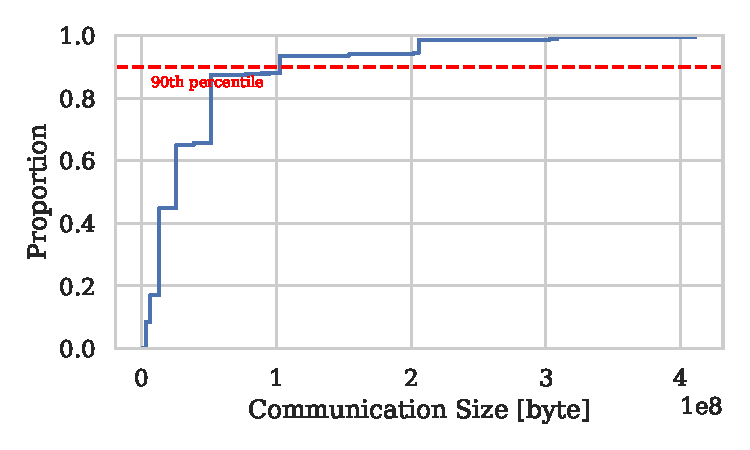
\includegraphics[width=0.85\textwidth]{./figure/4-alg/commmu_cdf.pdf}
	\caption{AmobaNet-D的计算图中通信代价的累积分布函数}
	\label{fig:commu-cdf}
\end{figure}

图\ref{fig:commu-cdf}展示了AmoebaNet-D模型的计算图中,所有边上的通信数据量的累积分布函数。
从图中可以发现,几乎$90\%$的通信数据量都低于$1\times 10^8$字节,大部分的通信都是较小的,只有少数的边具有较大的数据传输量,成为计算图中数据传输的瓶颈。
对于这类具有较大数据传输量的边,我们希望让边两端的节点被划分到相同设备上,从而避免边上较大的通信开销。

\sys{} 使用节点协同放置的方法,优先将通信开销较大的边两端的节点放置在同一个设备上。
一方面可以避免出现通信瓶颈,另一方面,可以有效减少约束优化中变量的个数。
\sys{}采用等价类(Equivalence Class)划分的思路对节点进行分组,
算法\ref{alg:co-place}描述了\sys{}进行节点协同放置的过程。

\begin{algorithm}[h]
	\caption{节点协同放置}
	\label{alg:co-place}
	\begin{algorithmic}[1]
	\REQUIRE 计算图:$\mathcal{G}$,设备列表:$\mathit{Devices}=\{p_1, p_2,\cdots, p_n\}$
	\ENSURE 节点到分组的映射: $\mathit{NodeToGroups}$
	\STATE $\mathit{NodeToGroups} \leftarrow \mathrm{Map}[\mathit{node}, \mathit{group}]$
	\STATE $\mathit{ds} \leftarrow \mathrm{NewDisjointSet}(\mathcal{G}.\mathcal{V})$
	\STATE $\mathit{totalMem}\leftarrow \sum_{i=1}^{n}p_i.\text{mem}$
	\STATE $\mathit{requireMem}\leftarrow \mathcal{G}.\text{mem}$
	\STATE $\mathit{maxGroupMem}\leftarrow \text{min}(\{p_1.\text{mem}, p_2.\text{mem}, \cdots, p_n.\text{mem}\})$
	\STATE $\mathit{minGroupNum}\leftarrow 2n$
	\IF{$\mathit{totalMem} < \mathit{requireMem}$}
		\STATE \textbf{RaiseError} "Insufficient Memory."
	\ENDIF
	\STATE $Q\leftarrow \text{SortByCommunicationSize}(\mathcal{G}.\mathcal{E})$ \quad\textcolor{gray}{\# 按照通信开销从大到小排序}
	\FOR{$\mathit{ds}.\mathit{size} \ge \mathit{minGroupNum}\quad \textbf{AND} \quad Q.\text{size} > 0$}
		\STATE $e\leftarrow Q.\text{pop()}$
		\IF{$\mathit{ds}.\text{Find}(e.u) = \mathit{ds}.\text{Find}(e.v)$}
			\STATE \textbf{continue}
		\ELSE
			\STATE $\mathit{newGroup} \leftarrow \mathit{ds}.\text{Find}(e.u) \cup \mathit{ds}.\text{Find}(e.v)$
			\IF{$\mathit{newGroup}.\text{mem} > \mathit{maxGroupMem}$}
				\STATE \textbf{continue} \quad \textcolor{gray}{\# 合并后NodeGroup过大,取消此次合并}
			\ELSE
				\STATE $\mathit{ds}.\text{Merge}(\mathit{ds}.\text{Find}(e.v, \mathit{ds}.\text{Find}(e.u)))$ \quad \textcolor{gray}{\# 进行合并}
			\ENDIF
		\ENDIF 
	\ENDFOR
	\FOR{$u\in \mathcal{G}.\mathcal{V}$}
		\STATE $\mathit{NodeToGroups}[u]\leftarrow \mathit{ds}.\text{Find}(u).\text{id}$
	\ENDFOR 
	\RETURN $\mathit{NodeToGroups}$
	\end{algorithmic}
\end{algorithm}


首先计算出计算图$\mathcal{G}$所需要的内存的总量和所有设备的可用内存,判断是否可以满足需求。
然后创建并查集(Disjoint Set),并查集是一种可以以接近常数时间复杂度的代价进行等价类的判断和合并的数据结构。
在初始化阶段,每个节点都位于不同的等价类中。
计算图中所有的边会按照通信代价从大到小进行排序,算法会优先检查通信代价较大的边,如果边两端的节点不属于同一个等价类,而且满足合并条件,则进行合并。
在合并过程中,节点组的数目不断减小,因此我们需要控制节点组的数目不会太小(小于设备数目),导致无法进行划分。
我们设置节点组的数目的下限为设备数目的2倍,当节点组数目低于下限时,停止合并。

当节点协同放置完成后,节点被分成了若干组。
同一组中的节点会被放置在同一个设备上,因此只需要简单修改约束优化问题\ref{eq:target},让同一组中的节点共享指示随机变量即可。
通过节点协同放置,\sys{}在进行约束优化的求解之前,将节点提前划分成了若干组,组内的节点共享指示随机变量,减少了带求解的变量的个数,可以有效减少求解的用时,并且提高求解的质量。

\subsection{实现:使用PICOS和Gurobi}
\label{sec:picos-implement}
本小节将介绍如何使用PICOS和Gurobi实现\ref{sec:core}中描述的约束优化问题的求解。

Gurobi \upcite{gurobi}是一款商业化的高性能线性规划(Linear Programming),整数规划(Integer Programming)和混合整数规划(Mixed Integer Programming)求解器。
Gurobi也可以用于二次规划(Quadratic Programming),具有高效、准确和灵活的特点,被广泛应用于各种优化问题的求解。
Gurobi采用了一系列优化技术和算法,如高效的分支界定算法、内点算法、割平面算法等,可以快速准确地求解各类优化问题。
作为商用求解器,Gurobi也提供了免费的学术许可证。
\sys{}使用Gurobi作为求解器,对\ref{sec:core}中描述的约束优化问题进行求解。

为了简化对Gurobi的使用,\sys{}使用PICOS \upcite{PICOS}作为Gurobi的前端。
PICOS的全称是“Python Interface for Conic Optimization Solvers”,它是Python的约束优化建模工具,它允许用户使用Python来对约束优化问题进行建模。
PICOS提供了方便的Python接口,用于构建和解决凸优化问题,它提供了符号表达式,约束组合等高级抽象方式来描述优化问题,在一定程度上可以简化约束优化问题的定义。
PICOS具有强大的可扩展性,支持包括Gurobi,MOSEK \upcite{mosek}等多种求解器作为约束优化问题求解的后端,PICOS可以自动将用户通过Python定义的约束优化问题转化为各个求解器的输入形式,并且调用求解器进行求解。

\begin{lstlisting}[language=Python, caption={约束优化求解的Python实现}]
import picos as pc
...
# 创建问题和优化目标
P = pc.Problem(name='NetSplit MQP Problem')
Makespan = pc.RealVariable(name='makespan', lower=0)
P.minimize = Makespan
# 为每个节点组创建指示随机变量
X = [[None,]*num_devices for _ in range(num_groups)]
for i in range(num_groups):
	for p in range(num_devices):
		X[i][p] = pc.IntegerVariable(lower=0,upper=1)
# 为每个节点声明变量S_fp, S_bp, C_fp, C_bp
S_fp, S_bp, C_fp, C_bp = [], [], [], []
for i in range(num_nodes):
	S_fp.append(pc.RealVaribel(lower=0.0))
	S_bp.append(pc.RealVaribel(lower=0.0))
	C_fp.append(pc.RealVaribel(lower=0.0))
	C_bp.append(pc.RealVaribel(lower=0.0))
...

# 约束1: 图的入口节点的前向传播开始时间为0
for i in entry_nodes:
	P.add_constraint(S_fp[i] == 0.0)
# 约束2: 图的出口节点反向传播开始时间等于前向传播结束时间
for i in exit_nodes:
	P.add_constraint(S_bp[i] == C_fp[i])
# 约束3: 每个节点的计算代价
for i in range(num_nodes):
	P.add_constraint(C_fp[i] == S_fp[i] + FP[i])
	P.add_constraint(C_bp[i] == S_bp[i] + BP[i])
# 约束4: Makespan大于所有节点完成反向传播
for i in range(num_nodes):
	P.add_constraint(Makespan >= C_bp[i])
# 约束5: 具有依赖关系的节点需要进行等待
for (i,j) in g.edges:
    P += S_fp[j] >= C_fp[i] + Commu[i][j]
    P += S_bp[i] >= C_bp[j] + Commu[i][j]
# 约束6: 每个Group只能被放在1个设备上
for group_idx in groups:
    P += pc.sum(X[group_idx]) == 1

P += Commu[u][v] >= pc.sum(comm_ij) 
... 
# 求解
P.solve(solver="gurobi")
# 获取结果
for i in range(num_groups):
	for p in range(num_devices):
		if X[i][p] == 1.0:
			group_to_device[i] = p
...
\end{lstlisting}

上面的代码展示了使用PICOS定义约束优化问题\ref{eq:target}的部分过程。
首先我们在代码中引入PICOS包,然后创建优化问题的实例\texttt{pc.Problem}。
然后我们定义一系列变量和优化问题的优化目标。
变量是表示优化问题中未知量的对象,在创建变量后可以进一步向问题中添加约束来描述变量应该满足的条件,在PICOS中,\texttt{RealVariable}和\texttt{IntegerVariable}是最常用的两种变量,分别用来表示连续的实数变量和整数型变量。
例如我们将指示每一个节点组放置的变量X定义为整数型变量,且它的值只能取到0或1,然后我们通过约束6来约束一个节点组要被放置且只能被放置在一个设备上。
在问题定义完成之后,调用\texttt{solve}方法,选择求解器,进行求解。

在\sys{}的约束优化问题\ref{eq:op-target}中,限制解的存在性的约束只有式\ref{eq:cons6},也就是显存约束。
当模型训练的显存用量超过设备可以提供的显存用量时,该优化问题无解。
当存在任意一种模型划分和放置方案可以满足显存约束时,则求解器一定可以寻找到该问题的一个解,在实际应用中,由于问题定义和数值精度等原因,该解不一定是最优解。
为了验证这种基于约束求解的模型划分方法的有效性,我们在后续章节(\ref{sec:evaluation})中对\sys{}得到的模型划分效果进行了评估。

\section{本章小结}
本章主要介绍了模型划分的问题的形式化定义以及基于约束优化的模型划分方法。
首先,我们在\ref{sec:formul} 中对问题进行了形式化的定义,模型的划分等同于计算图的划分,也就是寻找计算图中节点到设备的映射,以最大化模型训练时的数据吞吐量。
我们介绍了模型划分的输入以及对应的符号表示,并且论述了反向传播的用时对于模型划分的影响。
然后我们介绍了基于约束优化的模型划分方法,介绍了Pesto的约束优化问题的定义,并分析了Pesto的一些不足,例如未考虑反向传播用时对划分的影响,没有扩展到任意数目设备,没有考虑集群中通信链路的异构性等。
接着我们着重介绍了\sys{}的约束优化问题的定义和求解的实现。我们基于PICOS和Gurobi在Python中实现了问题的定义和求解。同时我们也介绍了用于优化通信的节点协同放置方法。

在后续章节(\ref{sec:evaluation})中,我们将介绍对\sys{}的实验评估。


\chapter{实验评估}
\label{sec:evaluation}

本章将介绍对\sys{}所进行的实验评估。
首先我们介绍实验设置(\ref{sec:setup}),包括所使用的硬件环境以及选取的模型和数据集。
然后是对\sys{}中提出的模型划分方法的性能评估(\ref{sec:performace})。
为了评估\sys{}中提出的模型划分方法的性能,我们在真实环境下选取了来自不同领域的深度神经网络模型,进行了模型并行化训练。
我们关注模型在不同的划分方法下的训练速度,训练速度越快,模型划分的效果越好。
接着为了验证\sys{}中的模型划分方法不会影响原始模型的收敛性,我们设计了训练收敛性验证实验(\ref{sec:convergence})。
我们会在每个实验中介绍实验的细节和结果,并且对结果进行分析。
最后我们对本章内容进行小结(\ref{sec:evaluation-summary})。

\begin{table}[!htbp]
	\centering
	\caption{服务器配置}
	\label{table:setup}
    \begin{tabularx}{0.9\linewidth}{ p{2.0cm} p{6.8cm} X}
        \toprule
        \textbf{配置项} & \textbf{型号} & \textbf{规格} \\
        \midrule
        GPU & Nvidia® TITAN RTX 24GB & 5 \\
        \midrule
        CPU & Intel® Xeon Gold 5118 @ 2.30GHz & 2 \\
        \midrule
        内存 & Samsung M393A4K40BB2-CTD  & 32GB $\times$ 12 \\
        \midrule
        操作系统 & Ubuntu & 4.15.0-88-generic \\
        \midrule
        \multirow{3}*{软件依赖} & PyTorch & 1.8.1 \\
        \cmidrule{2-3}
        & PICOS & 2.4.11 \\
        \cmidrule{2-3}
        & Gurobi & v10.0.0rc2 \\
        \bottomrule
    \end{tabularx}
\end{table}
\section{实验设置}
\label{sec:setup}
\subsection{硬件环境}
\label{sec:hardware}
\begin{table}[h!] % just use this specifier if really needed.
    \centering
    \caption{设备之间的通信拓扑}\label{table:topo}
    \begin{threeparttable}
    \begin{tabular}{ |p{1.5cm}| p{1.5cm}| p{1.5cm}| p{1.5cm}| p{1.5cm}| p{1.5cm}| }
        \hline
        & \textbf{GPU-0} & \textbf{GPU-1}& \textbf{GPU-2}& \textbf{GPU-3}& \textbf{GPU-4} \\
        \hline
        \textbf{GPU-0} & \texttt{X} & \texttt{PIX} & \texttt{NODE}&  \texttt{NODE}& \texttt{NODE} \\
        \hline
        \textbf{GPU-1} & \texttt{PIX} & \texttt{X} & \texttt{NODE} & \texttt{NODE} & \texttt{NODE} \\
        \hline
        \textbf{GPU-2} & \texttt{NODE} & \texttt{NODE} & \texttt{X} & \texttt{PIX} & \texttt{PIX} \\
        \hline
        \textbf{GPU-3} & \texttt{NODE}& \texttt{NODE} & \texttt{PIX} & \texttt{X} & \texttt{PIX} \\
        \hline
        \textbf{GPU-4} & \texttt{NODE}& \texttt{NODE} & \texttt{PIX}& \texttt{PIX} & \texttt{X}\\
        \hline
    \end{tabular}
    \begin{tablenotes}
        \item[1] \texttt{X}: 设备本身。
        \item[2] \texttt{PIX}: 设备之间通过单个PCIe switch连接。
        \item[3] \texttt{NODE}: 设备之间通过PCIe Host Bridge 在同一个NUMA节点内连接。
    \end{tablenotes}
    \end{threeparttable}
\end{table}

\begin{figure}[h]
	\centering
	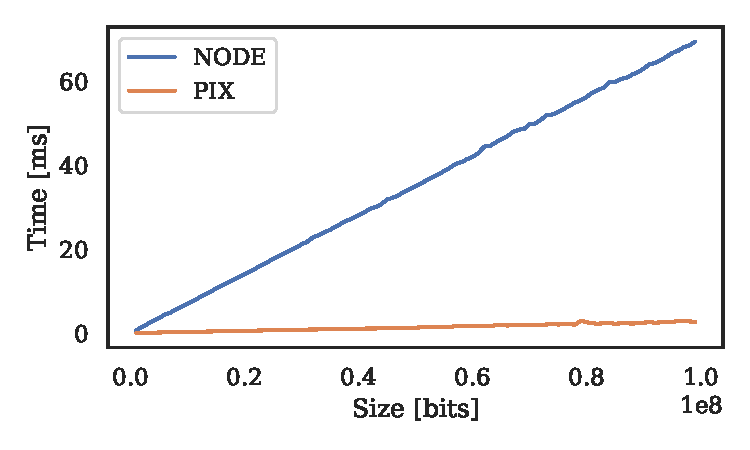
\includegraphics[width=0.75\textwidth]{./figure/5-evaluation/pix-vs-node.pdf}
	\caption{PCIe Switch和PCIe Bridge的通信速度对比}
	\label{fig:switch-vs-bridge}
\end{figure}

我们在一个服务器上进行实验,该服务器的配置如表\ref{table:setup}所示。
在该服务器上有5个型号相同GPU,每个GPU有24GB的显存,由于服务器上并未安装高性能的专用通信设备(例如NVLink)进行连接,因此GPU设备之间的通信链路是异构的,具体来说,GPU的通信拓扑如表\ref{table:topo}所示。


PCIe(Peripheral Component Interconect Express) 是一种高速串行接口总线标准,用于将各种外部设备(例如显卡,网卡,硬盘等)连接到计算机上。
在服务器上,设备之间连接的方式主要有\texttt{PIX}和\texttt{NODE}两种。
\texttt{PIX}是设备通过PCIe Switch使多个PCIe设备连接在一起。在这种方式下,设备共享同一条PCIe总线,设备与设备之间具有高带宽和高吞吐量的连接。
而在\texttt{NODE}连接方式中,设备所使用的PCIe总线通过PCIe Bridge设备连接到NUMA(Non-Uniform Memory Access)节点内的PCIe总线。由于设备之间不共享PCIe总线,所以设备之间的带宽和吞吐相比于\texttt{PIX}有所降低,但是这种方式由于不共享总线,所以具有更好的可扩展性。
图\ref{fig:switch-vs-bridge} 展示了在我们的实验环境中,\texttt{PIX}和\texttt{NODE}两种连接方式下,设备之间通信的速度对比。
图中横轴表示通信数据量,纵轴通信时间。
从图中可以看出,通过\texttt{PIX}方式连接的设备之间具有更高的通信速度,这也反映出了在真实环境中,设备之间通信方式的异构性。


\subsection{模型与数据集}
在实验中,我们需要比较不同的模型划分方法对于模型训练速度的影响。
为了说明\sys{}中的模型划分方法具有通用性,我们分别从图像分类领域和图像分割领域选择数据集和模型进行实验。

\noindent\textbf{数据集}:在数据集方面,我们选择来自图像分类领域的ImageNet数据集\upcite{imagenet} 和来自图像分割领域的VOC2012数据集\upcite{voc2012}。
\begin{itemize}
	\item ImageNet: 该数据集包含了来自1000个类别的超过120万张高分辨率图像,用于训练和评估图像分类模型。数据集中的每个图像都被进行了标记。ImageNet在图像分类竞赛和图像分类的研究论文中作为基准数据集被广泛使用,因此我们选取ImageNet作为我们的实验数据集之一。
	\item VOC2012: VOC2012是用于目标检测和图像分割领域的数据集,包含来自11500个来自20个不同类别的对象的图像,如人、汽车、动物等。图像中的每个对象都带有一个指定对象在图像中范围的边界框和一个指示对象类别的标签。VOC2012被广泛应用为目标检测和图像分割领域的基准数据集,我们选取VOC2012作为我们的实验数据集之一。
\end{itemize}

\noindent\textbf{模型}: 在模型方面,我们在图像分类模型和图像分割模型中各选择两个大模型进行实验。在图像分类模型中,我们选择AmoebaNet-D\upcite{amoebanet} 和 Wide ResNet-152\upcite{wide}。在图像分割模型中,我们选择了U-Net\upcite{unet} 和DeepLab-V3\upcite{deeplabv3}。
\begin{itemize}
	\item AmoebaNet-D: AmoebaNet-D是AmoebaNet卷积神经网络架构的一种。它使用神经结构搜索算法(Neural Architecture Search, NAS)\upcite{nas} 设计,该算法可以根据给定任务自动搜索合适的网络结构。AmoebaNet-D的特点是具有大量的卷积层和复杂的模型结构,这使其可以学习到复杂的特征,因此AmoebaNet-D在图像分类任务上取得了很好的性能。
	\item Wide ResNet-152: 残差网络(Residual Network)是一种使用残差连接的深度神经网络,ResNet-152\upcite{resnet} 是残差网络的一种,它有152层,包括卷积、池化和全连接的组合。在相关研究\upcite{wide}中,研究者将ResNet中的卷积算子的通道数扩大后发现模型的性能得到了提高。我们在实验中将通道数ResNet-152的通道数扩大2倍,作为我们的待测模型。
	\item U-Net: U-Net是一种用于图像分割任务的卷积神经网络架构,其架构中包括一个对图像进行下采样的编码器和一个对图像进行上采样的解码器,通过采样可以让U-Net捕捉到图像在不同层次下的特征,目前U-Net已经被广泛应用于图像分割任务中。
	\item DeepLab-V3: DeepLab-V3是一种基于编码器/解码器结构的图像分割模型,通常,DeepLab-V3中,使用ResNet等其他卷积神经网络作为编码器,提取图像的特征,然后使用解码器从特征中生成分割结果。我们在实验中使用 Wide ResNet-152作为DeepLab-V3的编码器。
\end{itemize}
表\ref{table:model} 展示了我们所选用的模型在输入图片为$224\times 224$分辨率下,数据批大小为128时的内存需求,从表中可以看出,这些模型的内存需求已经远远超出我们的实验环境中的单个设备的内存容量(24GB)。

\begin{table}[h!] % just use this specifier if really needed.
    \centering
    \caption{模型内存需求}\label{table:model}
    \begin{tabularx}{0.86\linewidth}{ p{3.5cm} p{3.5cm} X  }
        \toprule 
        \textbf{模型名称} & \textbf{计算图节点数目} & \textbf{内存需求(MB)} \\
        \midrule 
        AmoebeNet-D & 784 & 117756.06 \\
        Wide ResNet-152 & 388 & 115179.77 \\
        U-Net & 134 & 50121.92 \\
        DeepLab-V3 & 417 & 168094.43 \\
        \bottomrule
    \end{tabularx}
\end{table}


\section{训练性能验证}
\label{sec:performace}
\subsection{对比方法}
为了验证\sys{}对于使用模型并行化对大模型进行训练的效果,我们引入了其他四种方法和\sys{}进行对比。
\begin{itemize}
	\item \texttt{m-TOPO}: \texttt{m-TOPO}是Baechi\upcite{baechi}提出的三种模型划分放置算法之一,全称为Memory-Constrained Topological Sort Placer。该算法的思路是对计算图中所有的节点进行拓扑排序,然后依次放置在当前设备上,直到达到当前设备的内存容量限制,再转向下一个设备继续放置。Baechi中将设备的内存容量限制设置为$\sum_{i\in\{n\}}d_i / m + \mathrm{max}_{i\in\{n\}} d_i$,其中$m$为设备数目,$d_i$为节点$i$的内存用量。通过这种方式,可以控制每个设备具有近似的内存用量。
	\item \texttt{m-ETF}: \texttt{m-ETF}是Baechi\upcite{baechi} 中提出的另一种模型划分放置算法,全称为Memory-Constrained Earliest Task First。该算法在最早任务优先调度算法\upcite{etf} 的基础上改进得到。该算法维护一个队列,队列中放置着所有的节点和设备的组合$(i,p)$,其中$i$表示节点,$p$表示设备。$(i,p)$按照最早可调度时间升序排列,最早可调度时间的计算按照式\ref{eq:etf}得到。
	\begin{equation}
		\label{eq:etf}
		\mathrm{ETF}(i,p) = \max\left[\mathit{free(p)}, \max_{i\in \Gamma^- (j)}(s_i+k_i+c_{ij}x_{ip}) \right]
	\end{equation}
	式\ref{eq:etf}中,节点$i$在设备$p$上的最早可调度时间为设备$p$的空闲时间和节点$i$的所有前驱节点$j$完成用时中的最大值。
	\texttt{m-ETF}依次从队列中取出当前可调度时间最小的组合$(i,p)$,如果设备$p$的剩余内存可以放置节点$i$,则将节点$i$放置到设备$p$,并更新设备$p$的空闲时间$\mathit{free}(p)$和$i$的所有后继的最早可调度时间。重复这个过程直到所有节点都被调度。

	\item \texttt{m-SCT}: 该算法是在经典的调度算法最小通信时间调度\upcite{sct}上改进得到。在\texttt{m-SCT}中,首先通过整数线性规划(Integer Linear Program)以最小化整体完成时间为目标,为每个节点寻找一个最优子节点,并优先将节点和其最优子节点放置在同一个设备上。
	\item \texttt{Pesto}: 同时,我们也对比了\texttt{Pesto}和我们的方法,由\texttt{Pesto}的原始约束优化问题(\ref{sec:pesto})只能适用于设备数目为2的情况,我们对其进行了扩展。我们采用和\sys{}类似的方法,使用多个指示变量来表示节点在设备上的放置。修改后的\texttt{Pesto}的约束优化问题定义为式\ref{eq:p-target-2}。
\end{itemize}


\begin{align}
	& \text{min} & & \mathit{Makespan} \label{eq:p-target-2} & \\
	& \text{s.t.} & & \mathcal{S}_{i}=0 &\Gamma^{-}(i)=0, i\in \mathcal{V} \nonumber\\
	& & & \mathcal{C}_{i} = \mathcal{S}_{i} + \mathit{p}_i & \forall i\in \mathcal{V} \nonumber\\
	& & & \mathit{Makespan} \ge \mathcal{C}_{i} & \forall i\in \mathcal{V}\nonumber\\
	& & & \sum_{p=1}^{m} \mathcal{X}_{i,p}=1, \mathcal{X}_{i,p}\in\{0,1\} & \forall i\in \mathcal{V} \nonumber\\
	& & & \mathit{Commu}_{i,j} = \sum_{p\neq q}\mathcal{X}_{i,p}\mathcal{X}_{j,q}F_{\mathit{commu}}(i,j,p,q) & \forall \left\langle i,j\right\rangle \in \mathcal{E} \nonumber\\
	& & & \mathcal{S}_{j} \ge \mathcal{C}_{i} + \mathit{Commu}_{i,j}&\forall \left\langle i,j\right\rangle \in \mathcal{E} \nonumber
\end{align}




% \section{实验结果}
% 本节将介绍\sys{}和其他模型划分方法在性能上的对比(\ref{sec:performace})。此外,为了验证\sys{}并不会影响模型的收敛性,还将在\ref{sec:convergence}中对模型训练的收敛性进行验证,最后会在\ref{sec:partition-result}展示模型划分的效果图。

\subsection{实验结果及分析}


\begin{figure}[ht]
	\centering
	\begin{subfigure}[b]{0.45\textwidth}
	  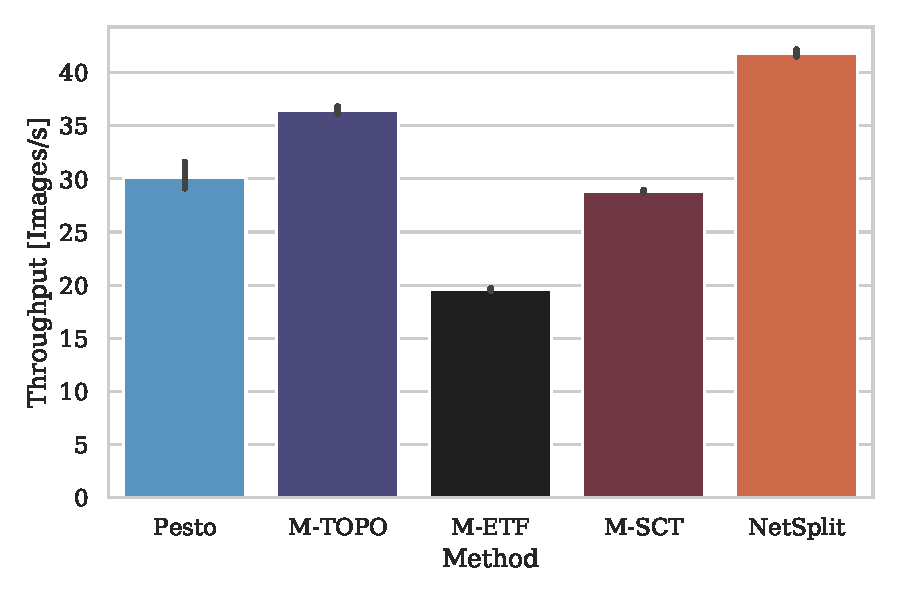
\includegraphics[width=\textwidth]{./figure/5-evaluation/result-amoebanetd.pdf}
	  \caption{AmoebaNet-D}
	\end{subfigure}
	\quad
	\begin{subfigure}[b]{0.45\textwidth}
	  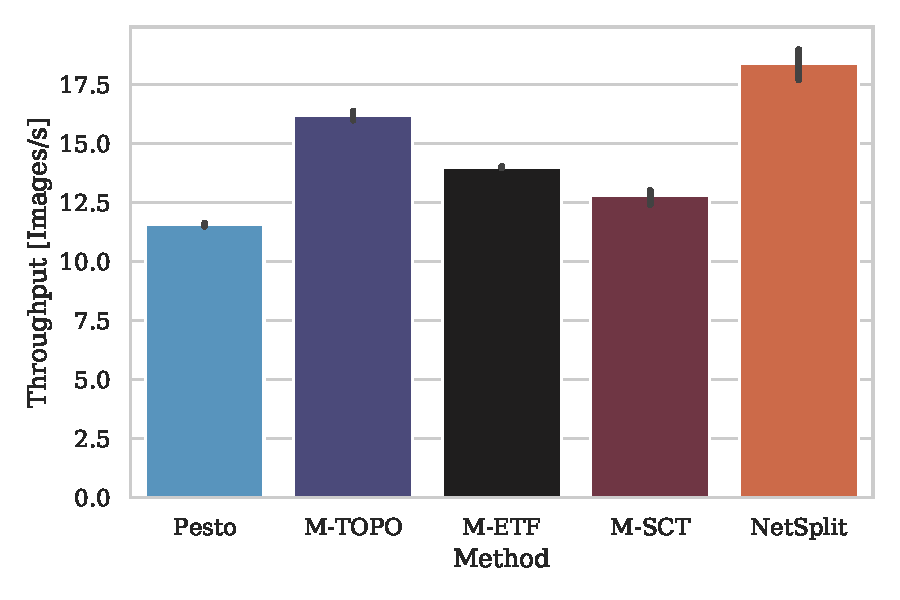
\includegraphics[width=\textwidth]{./figure/5-evaluation/result-deeplabv3.pdf}
	  \caption{DeepLab-V3}
	\end{subfigure}
	\vskip\baselineskip
	\begin{subfigure}[b]{0.45\textwidth}
	  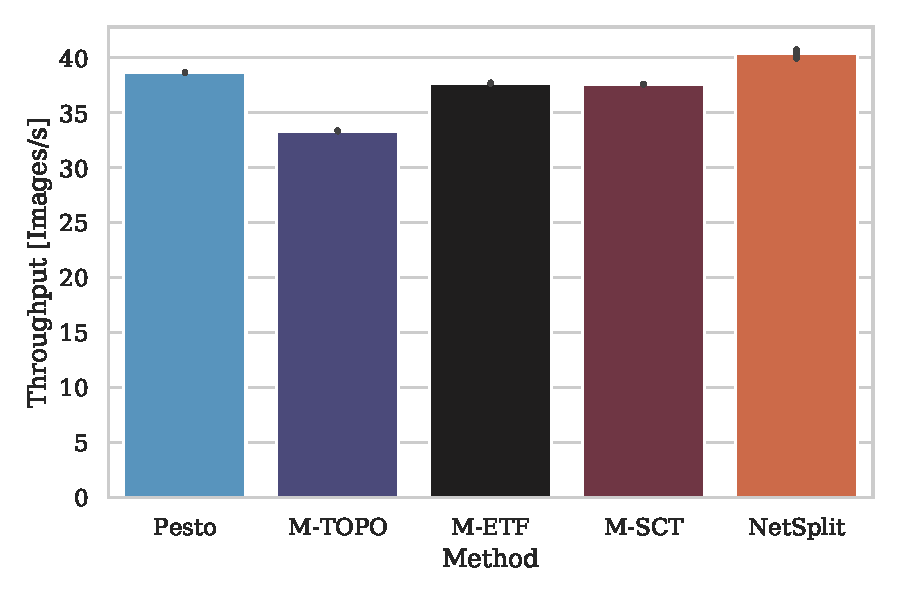
\includegraphics[width=\textwidth]{./figure/5-evaluation/result-unet.pdf}
	  \caption{U-Net}
	\end{subfigure}
	\quad
	\begin{subfigure}[b]{0.45\textwidth}
	  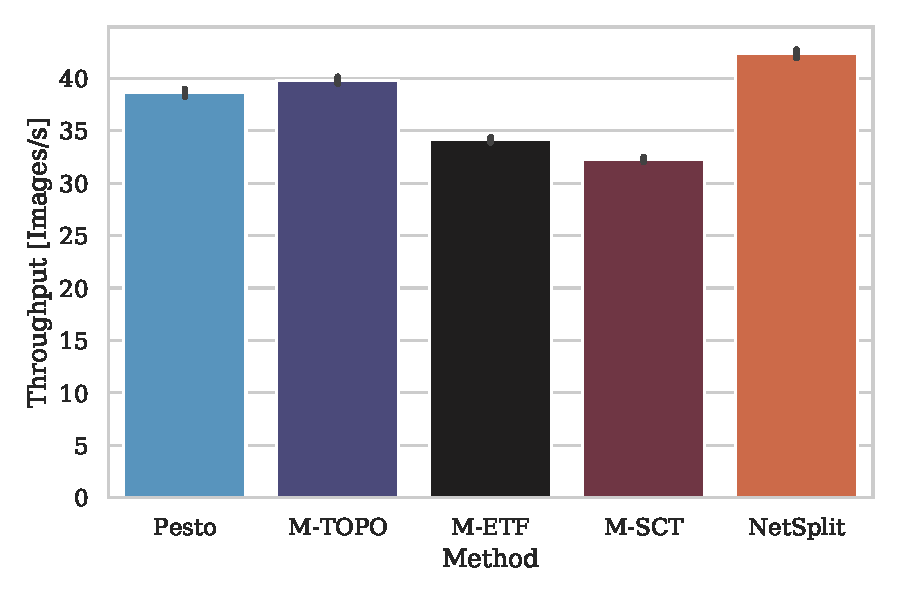
\includegraphics[width=\textwidth]{./figure/5-evaluation/result-wide-resnet152.pdf}
	  \caption{Wide ResNet-152}
	\end{subfigure}
	\caption{\sys{}和其他模型划分方法在4个不同模型上的对比}
	\label{fig:result}
\end{figure}

我们选择\ref{sec:setup}中提到的模型和数据集进行训练,并在训练过程中采集100个数据批的训练用时,计算出每个数据批的平均用时和数据吞吐量。
我们选用3个GPU对每个模型进行训练,其中GPU-0和GPU-1以及GPU-2之间通过\texttt{NODE}的方式进行连接,GPU-1和GPU-2之间通过\texttt{PIX}的方式进行连接。
对于每一个模型,具体的配置为:
\begin{itemize}
	\item AmoebaNet-D: 我们使用18层的AmoebaNet-D,在ImageNet数据集上进行训练,数据批大小设置为64。
	\item Wide ResNet-152: 使用ImageNet数据集进行训练,数据批大小设置为64。
	\item U-Net: 使用VOC2012数据集进行训练,数据批大小设置为128。
	\item DeepLab-V3: 使用VOC2012数据集进行训练,数据批大小设置为48。
\end{itemize}

图\ref{fig:result} 展示了在相同的硬件环境下,在不同模型上使用不同的模型划分方法进行模型并行化训练时数据吞吐量的对比。
从图中可以看出,几种对比方法在不同的模型上表现各有优劣。而相比于几种对比方法,\sys{}在不同的模型上都获得了更高的数据吞吐量,可以在单位时间内完成更多的样本数据的训练,因此可以有效的提升训练速度。

\begin{table}
    \centering
    \caption{性能比较}\label{table:performance}
    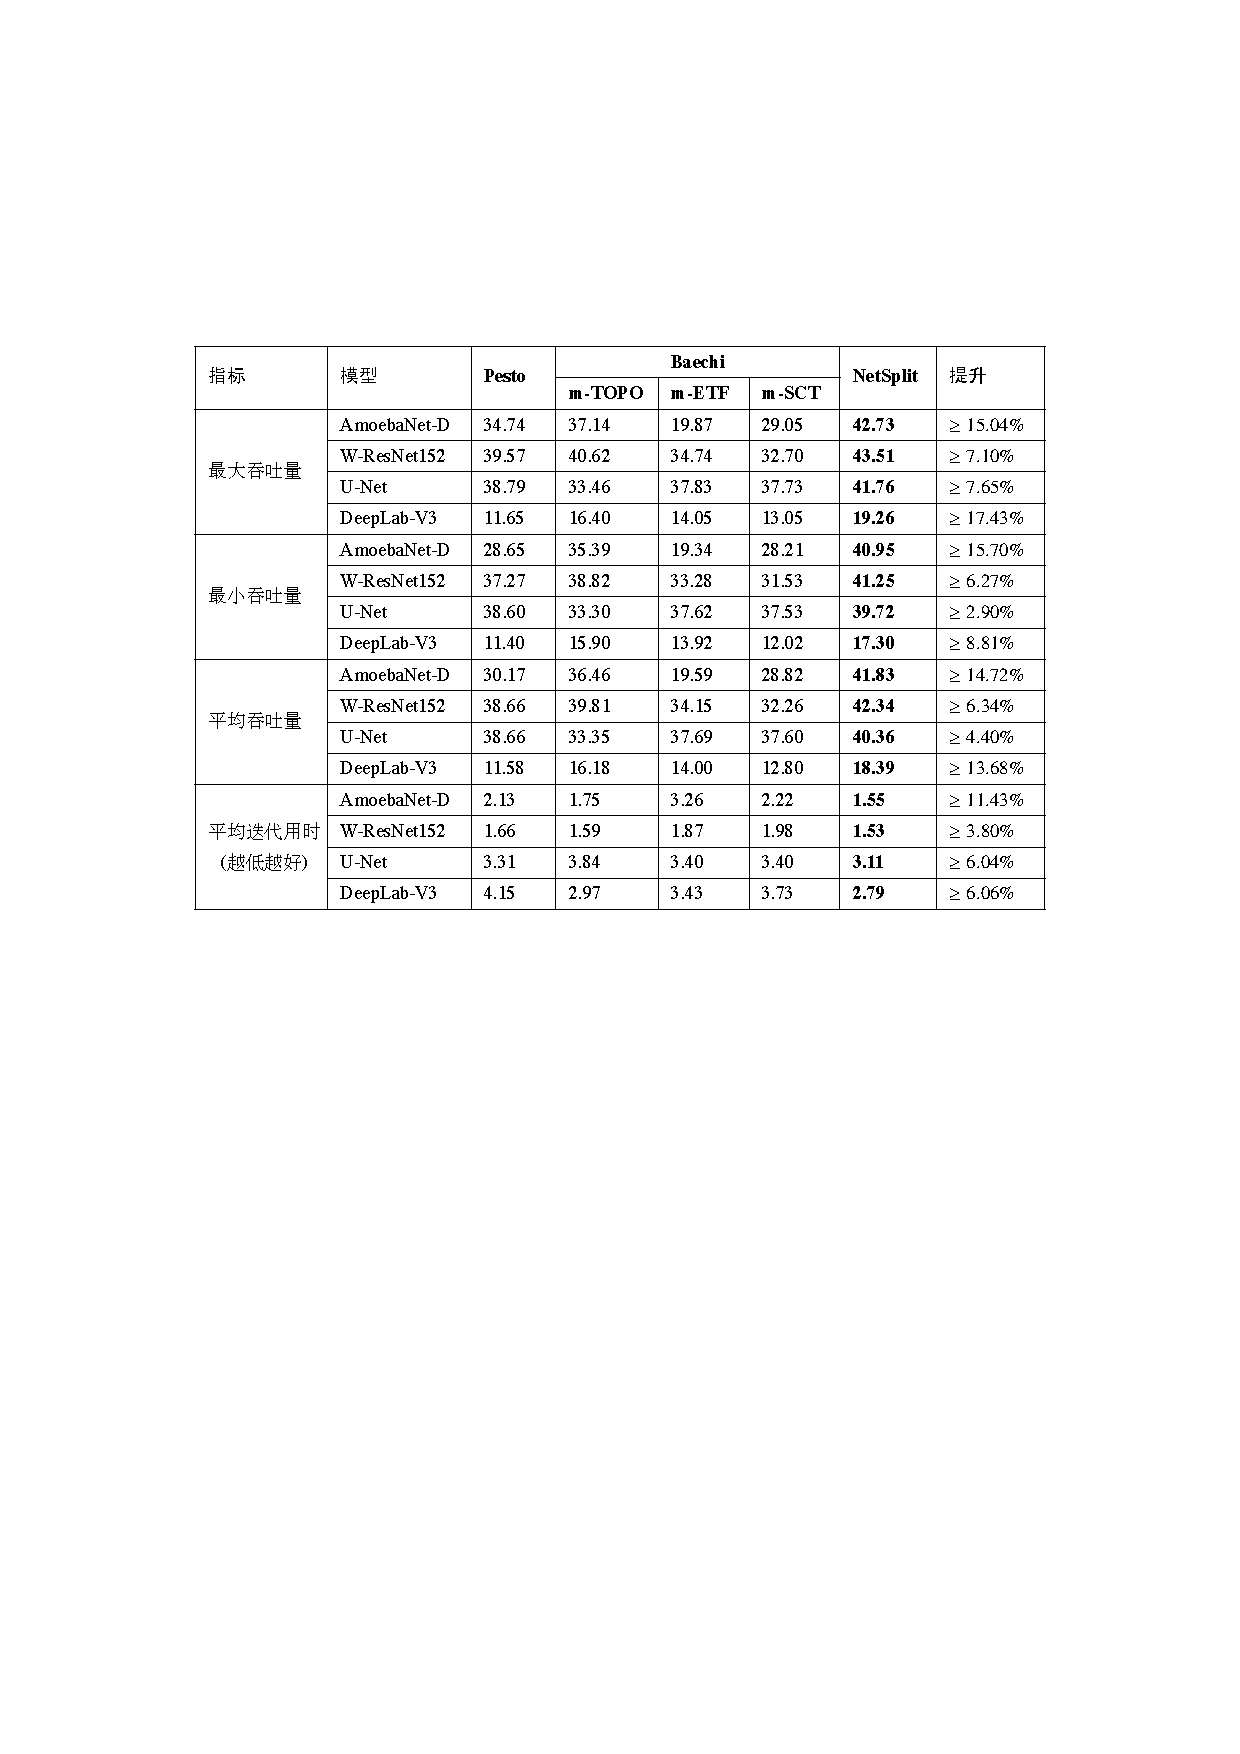
\includegraphics[width=0.98\textwidth]{figure/5-evaluation/performance-table.pdf}
\end{table}

% \begin{table}[h!] % just use this specifier if really needed.
%     \centering
%     \caption{性能比较}\label{table:performance}
%     \tiny
%     \begin{tabular}{ |p{1.8cm} |p{2.0cm} |p{1.0cm} |p{1.3cm} |p{1.1cm} |p{1.1cm} |p{1.2cm} |p{1.4cm}| }
%         \hline
%         \multirow{2}{*}{\textbf{指标}} & \multirow{2}{*}{\textbf{模型}} & \multirow{2}{*}{\textbf{Pesto}} & \multicolumn{3}{c|}{\textbf{Baechi}} & \multirow{2}{*}{\textbf{NetSplit}}  & \multirow{2}{*}{\textbf{提升}}  \\ 
%         \cline{4-6} 
%         & & &\textbf{m-TOPO} & \textbf{m-ETF} & \textbf{m-SCT} & &\\  
%         \hline
%         \multirow{4}{*}{最大吞吐量} & AmoebaNet-D  &  34.74 & 37.14 & 19.87 & 29.05 & \textbf{42.73} & $\ge 15.04\%$ \\
%                                   \cline{2-8}
%                                   & W-ResNet152 &39.57 & 40.62 & 34.74 & 32.70 & \textbf{43.51} & $\ge 7.10\%$ \\
%                                   \cline{2-8}
%                                   & U-Net          &38.79 & 33.46 & 37.83 & 37.73 & \textbf{41.76} & $\ge 7.65\%$ \\
%                                   \cline{2-8}
%                                   & DeepLab-V3    &11.65 & 16.40 & 14.05 & 13.05 & \textbf{19.26} & $\ge 17.43\%$ \\
%         \hline
%         \multirow{4}{*}{最小吞吐量} & AmoebaNet-D  &  28.65 & 35.39 & 19.34 & 28.21 & \textbf{40.95} & $\ge 15.70\%$ \\
%                                   \cline{2-8}
%                                   & W-ResNet152 &37.27 & 38.82 & 33.28 & 31.53 & \textbf{41.25} & $\ge 6.27\%$ \\
%                                   \cline{2-8}
%                                   & U-Net          &38.60 & 33.30 & 37.62 & 37.53 & \textbf{39.72} & $\ge 2.90\%$ \\
%                                   \cline{2-8}
%                                   & DeepLab-V3    &11.40 & 15.90 & 13.92 & 12.02 & \textbf{17.30} & $\ge 8.81\%$ \\
%         \hline
%         \multirow{4}{*}{平均吞吐量} & AmoebaNet-D  & 30.17 & 36.46 & 19.59 & 28.82 & \textbf{41.83} & $\ge 14.72\%$ \\
%                                   \cline{2-8}
%                                   & W-ResNet152 &38.66 & 39.81 & 34.15 & 32.26 & \textbf{42.34} & $\ge 6.34\%$ \\
%                                   \cline{2-8}
%                                   & U-Net         &38.66 & 33.35 & 37.69 & 37.60 & \textbf{40.36} & $\ge 4.40\%$ \\
%                                   \cline{2-8}
%                                   & DeepLab-V3     &11.58 & 16.18 & 14.00 & 12.80 & \textbf{18.39} & $\ge 13.68\%$ \\
%         \hline
%         \multirow{4}{*}{\makecell{平均迭代用时\\(越低越好)}} & AmoebaNet-D    &2.13& 1.75& 3.26& 2.22&  \textbf{1.55} &  $\ge 11.43\%$\\
%                                                          \cline{2-8}
%                                                         & W-ResNet152 & 1.66& 1.59& 1.87& 1.98& \textbf{1.53} & $\ge 3.80\%$\\
%                                                          \cline{2-8}
%                                                         & U-Net          & 3.31& 3.84& 3.40& 3.40& \textbf{3.11} & $\ge 6.04\%$ \\
%                                                          \cline{2-8}
%                                                         & DeepLab-V3     & 4.15& 2.97& 3.43& 3.73& \textbf{2.79} & $\ge 6.06\%$\\
%         \hline
%     \end{tabular}
% \end{table}


% \begin{table}[h!] % just use this specifier if really needed.
%     \centering
%     \caption{性能比较}\label{table:performance}
%     \tiny
%     \begin{tabularx}{\linewidth}{ p{1.4cm} p{1.7cm} p{1.4cm} p{1.4cm} p{1.4cm} p{1.4cm} p{1.4cm} p{1.2cm}}
%         \toprule 
%         \multirow{2}{*}{\textbf{指标}} & \multirow{2}{*}{\textbf{模型}} & \multirow{2}{*}{\textbf{Pesto}} & \multicolumn{3}{c}{\textbf{Baechi}} & \multirow{2}{*}{\textbf{NetSplit}}  & \multirow{2}{*}{提升}\\ 
%         \cmidrule{4-6} 
%         & & &\textbf{m-TOPO} & \textbf{m-ETF} & \textbf{m-SCT} & \\  
%         \midrule
%         \multirow{4}{*}{最大吞吐量} & AmoebaNet-D    & & & & & & \\
%                                   \cmidrule{2-8}
%                                   & W-ResNet152 & & & & & & \\
%                                   \cmidrule{2-8}
%                                   & U-Net          & & & & & & \\
%                                   \cmidrule{2-8}
%                                   & DeepLab-V3     & & & & & & \\
%         \midrule
%         \multirow{4}{*}{最小吞吐量} & AmoebaNet-D    & & & & & & \\
%                                   \cmidrule{2-8}
%                                   & W-ResNet152 & & & & & & \\
%                                   \cmidrule{2-8}
%                                   & U-Net          & & & & & & \\
%                                   \cmidrule{2-8}
%                                   & DeepLab-V3     & & & & & & \\
%         \midrule
%         \multirow{4}{*}{平均吞吐量} & AmoebaNet-D    & & & & & & \\
%                                   \cmidrule{2-8}
%                                   & W-ResNet152 & & & & & & \\
%                                   \cmidrule{2-8}
%                                   & U-Net          & & & & & & \\
%                                   \cmidrule{2-8}
%                                   & DeepLab-V3     & & & & & & \\
%         \midrule
%         \multirow{4}{*}{平均迭代用时} & AmoebaNet-D    & & & & & & \\
%                                     \cmidrule{2-8}
%                                     & W-ResNet152 & & & & & & \\
%                                     \cmidrule{2-8}
%                                     & U-Net          & & & & & & \\
%                                     \cmidrule{2-8}
%                                     & DeepLab-V3     & & & & & & \\
%         \bottomrule
%     \end{tabularx}
% \end{table}

表\ref{table:performance}展示了几种不同的模型划分方式下,进行模型并行化训练时的性能比较。
对比表中的数据我们发现,\sys{}和其他的方法相比,在不同的模型和数据集上,可以有效提升平均数据吞吐量$4.4\% \sim 14.72\%$,相应的,平均迭代用时,也就是模型训练每个数据批的时间减少了$3.8\% \sim  11.43\%$。
由于采样误差和训练过程中其他开销(数据预处理,磁盘IO等)的影响,导致平均数据吞吐量的提升和平均迭代用时的减少略有一些差异。
总的来说,相比于其他方法,使用\sys{}进行模型划分,可以有效提升模型并行化的训练效率,提升集群中的硬件资源利用率,缩短训练任务的用时。


在几种被测模型中,对于模型大小更大的AmoebaNet-D和DeepLab-V3,\sys{}的表现最好,相比于其他几种方法,在吞吐量方面有超过$13.68\%$的提升。
而对于模型大小较小的U-Net,\sys{}相比于其他几种方法中表现最好的\texttt{Pesto}来说,提升只有$4.40\%$。
对于AmoeBaNet-D和DeepLab-V3这种计算图中含有大量节点和边的复杂模型,在进行训练时,设备需要进行大量运算来得到反向传播的中间结果。同时由于模型的计算图中有大量的边,导致模型训练过程的实际通信代价较大,因此针对异构通信环境并且在约束优化问题的求解中加入反向传播的\sys{}在这样的复杂模型上表现更好。而没有考虑反向传播用时和异构的通信环境的\texttt{Pesto}在面对这样的复杂模型时,性能反而不如一些近似算法。

\subsection{有效性威胁分析}
\label{sec:threat}
% 1. 我们在单个主机的多个设备上进行实验,在这种情况下,p2p通信只发生在设备内部。尽管我们没有将实验扩展到多个主机的多个设备,并且让部分通信发生在网络上,但是这并不会影响建模准确性。因为即使是在单个主机上,设备之间的通信链路也是异构的,从实验结果上,在单机上有效
% 2. 在数据集和模型的选择上,我们选择来自图像领域的模型和数据集,而没有选择如文字、音频和视频等数据集。why? 图像识别有代表性,不同的任务领域的训练模式和特征是一样的,都是迭代式训练。


在实验场景的选择上,在\sys 对于模型训练性能的提升的实验评估中,我们将模型划分到位于单个主机的多个设备上进行训练,此时设备之间的通信只发生在主机的内部。而在真实的模型训练场景下,模型有可能被划分到位于多个主机的多个设备上,这种情况下,部分通信通过主机之间互联的网络进行。因此在单机场景下的实验也许无法反映真实场景下不同方法的性能差距。但是在单个主机上,设备之间的通信链路也是异构的,例如设备之间有可能通过PCIe Switch 连接,也有可能通过PCIE Host Bridge 连接,这种异构性和真实场景下的通信类似,因此,\sys 中对于问题的建模可以用于真实的场景。未来可以尝试更加真实场景下的设备和通信方式。



在数据集和模型的选择上,我们选择了图像领域的模型和数据集作为实验对象,因此,我们尚不清楚我们的框架在其他领域的模型和数据集的效果如何。但由于图像识别是最具有代表性、最被广泛研究的深度学习任务之一,并且我们选择的模型和数据集都是广泛被使用的基准测试,我们相信我们的评估结果在一定程度上是可靠的。我们将在未来工作中增加对文本、音频、视频等领域模型和数据集的评估。


\section{训练收敛性验证}
\label{sec:convergence}
我们设计了训练收敛性实验来验证\sys{}中对模型所进行的转换操作以及模型划分操作不会影响原始模型的性能。

\subsection{对比方法}
\begin{table}[h!] % just use this specifier if really needed.
    \centering
    \caption{收敛性验证实验配置}\label{table:convergence-setup}
    \begin{tabularx}{0.66\linewidth}{ p{3.5cm} X  }
        \toprule 
        \textbf{配置项} & \textbf{配置值}\\
        \midrule 
        模型 & ResNet-152 \\
        数据集 & ImageNet \\
        数据批大小 & 64 \\ 
        设备数目 & 4 \\
        学习率 & 1e-4 \\ 
        优化器 & Adam Optimizer \\
        \bottomrule
    \end{tabularx}
\end{table}

如本文\ref{sec:convertion} 中所述,当用户向\sys{}提交以PyTorch中\texttt{nn.Module}格式定义的模型后,\sys{}会将用户的模型转化成计算图的中间表示,在划分完成后,\sys{}还会将中间表示转化成\texttt{fx.GraphModule}。
在进行第二步转化时,会在模型中根据划分结果插入一些额外的节点,完成跨设备的变量转移。
因此为了验证经过多次转化和修改后的模型是否还和原模型在功能上等价,我们设计了收敛性验证实验。

收敛性验证实验的目的是为了验证\sys{}并不会损害原始模型的性能,我们通过测试使用\sys{}训练转换后的模型和使用数据并行化(Data Parallelism, DP)训练的原始模型的收敛性进行验证。
对于数据并行化,我们使用PyTorch中提供的DistributedDataParallel(DDP)\footnote{\url{https://pytorch.org/docs/stable/notes/ddp.html}} 进行训练。
我们使用的实验配置如表\ref{table:convergence-setup} 所示。


\subsection{实验结果及分析}

图\ref{fig:convergence-all} 展示了模型收敛性的验证结果。
其中,图\ref{fig:convergence-epoch}展示了在两种不同的训练方式下,模型的准确率随着训练轮次(Epoch)变化的情况。
我们一共训练了40个轮次,从图中可以看出,在相同的轮次下,两种训练方式得到的模型的准确率几乎相同。
因此可以得到结论,\sys{}并不会损害原始模型的性能,即不会影响原始模型的收敛性。
此外,图\ref{fig:convergence-time} 展示了模型的准确率随着时间的变化情况。
可以看出,由于\sys{}利用了模型并行化方法,有效提升了大模型训练的效率,相比于数据并行化方法,每一轮所需的训练时间更短,模型随着时间的收敛速度更快。

\begin{figure}[ht]
	\centering
	\begin{subfigure}[b]{0.85\textwidth}
	  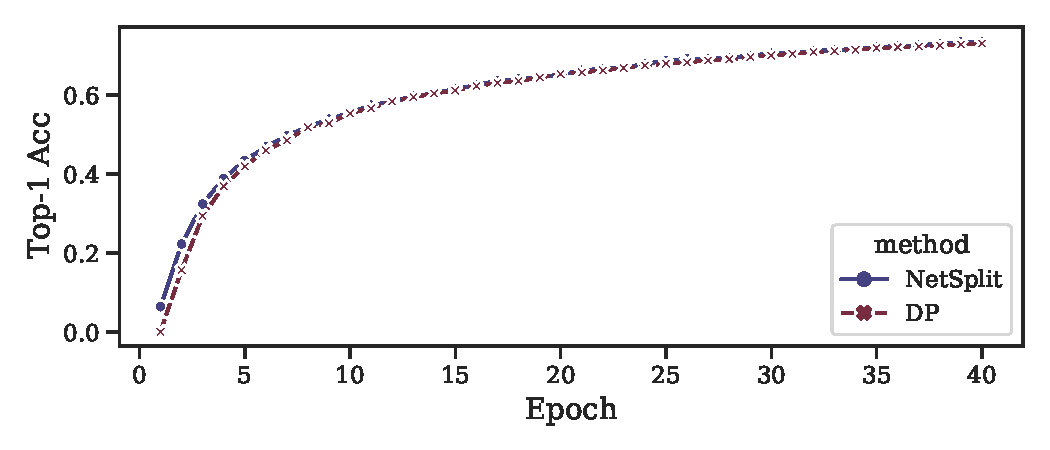
\includegraphics[width=\textwidth]{./figure/5-evaluation/convergence-epoch.pdf}
	  \caption{模型准确率随轮次(Epoch)变化}
	  \label{fig:convergence-epoch}
	\end{subfigure}
	\vskip\baselineskip
	\begin{subfigure}[b]{0.85\textwidth}
	  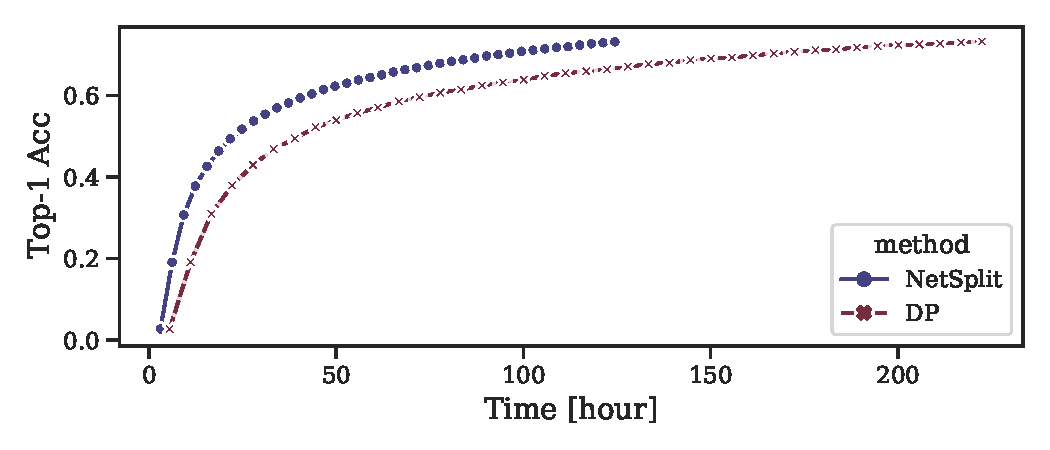
\includegraphics[width=\textwidth]{./figure/5-evaluation/convergence-time.pdf}
	  \caption{模型准确率随时间变化}
	  \label{fig:convergence-time}
	\end{subfigure}
	\caption{收敛性验证}
	\label{fig:convergence-all}
\end{figure}


\section{本章小结}
\label{sec:evaluation-summary}

在本章中,我们详细介绍了针对\sys{}进行的两方面实验,分别是训练性能验证和训练收敛性验证。
训练性能验证实验中,我们将\sys{}和其他的模型并行化方法在真实的模型和数据集上进行训练,通过比较训练时的数据吞吐量来评估训练性能。
实验结果表明,相比于已有方法,\sys{}可以有效提升对大模型进行模型并行化训练的训练效率,缩短训练任务用时。
在训练收敛性验证实验中,我们比较\sys{}和数据并行化的对在相同条件下对同一个模型的训练过程,实验结果表明\sys{}不会影响模型训练过程的收敛性。

下一章(\ref{sec:summary})将总结本文的工作,并展望未来的工作。

\chapter{总结与展望}
\label{sec:summary}

\section{工作总结}
近年来,深度学习技术成为了人工智能领域发展最快的分支之一。
得益于大数据时代的爆发式数据增长,深度神经网络模型可以获得海量高质量训练数据。
深度学习广泛应用在不同的领域中,并取得了成功。
然而随着深度神经网络模型性能的提高,模型的复杂度和参数量也迅速增长,导致单个计算设备无法训练完整的模型,因此为了对大模型进行训练,将模型划分到多个设备上进行并行化训练的模型并行化技术出现。

进行模型并行化训练需要对模型进行合理的划分,目前流行的深度学习框架PyTorch中,仍然依赖使用者对模型进行手动划分。
而对于大型神经网络模型来说,由于模型规模大,手动划分十分困难。
因此一些自动化的模型划分方法被提出,但是现有的方法仍然存在一些问题,例如没有在模型划分的过程中考虑底层硬件环境特点,模型划分粒度较粗,没有对模型训练过程进行精确建模等。

针对上述问题,为了更好的提供模型的自动划分和大模型的训练功能,本文提出并实现了一种针对大型神经网络的训练框架:\sys{}。
\sys{}基于PyTorch实现,并且可以接受通用的PyTorch神经网络模型。
对于输入的模型,\sys{}首先解析模型底层的计算图,并将其转化为一种中间表示。
然后对于计算图,\sys{}通过动态分析和静态分析的方式,获取图中每个节点的计算时间和内存用量等模型元信息。
同时,\sys{}也会采集底层硬件信息,获取设备之间的通信代价模型。
\sys{}将依据模型元信息和硬件信息,以提升训练效率为目标,对模型进行划分,然后将划分后的模型放置到设备上进行训练。
具体贡献包括:
\begin{enumerate}
	\item 实现了自动化的模型分析方法:由于PyTorch中的计算图在运行时动态生成,因此PyTorch的模型难以进行静态分析和划分。我们设计了模型转换模块,可以完成PyTorch模型和计算图中间表示的双向转换。并基于模型转换模块实现了自动化的模型分析,提取出对于模型划分有帮助的模型元信息。
	\item 实现了对底层设备之间通信的建模:参与模型并行化训练的多个设备之间需要进行通信,而在集群中,设备之间的通信方式往往是异构的。结合底层设备之间通信的异构性有助于得到更好的划分效果。我们设计了通信建模模块,可以对底层设备之间的通信进行建模。
	\item 实现了基于约束优化求解的模型划分方法:\sys{}形式化的定义了模型划分问题,使用基于约束优化求解的方法,以最小化单次迭代时间为目标,进行约束求解。相比于现有方法,\sys{}中的约束求解考虑了反向传播的代价,并且对底层的通信进行了更精确的描述。
	\item 通过实验对\sys{} 进行了验证:我们在真实的数据集和模型上对比了\sys{}和其他的模型划分方法,实验结果验证了\sys{}可以有效提升大模型进行模型并行化训练的训练效率,缩短模型训练用时,同时不会影响模型训练过程的收敛性。
\end{enumerate}


\section{工作展望}

本文中提出的模型并行化训练框架\sys{},简化大模型的模型并行化训练过程,有效提升大模型的训练效率,
但是仍然有需要进一步改进的方向。

本文中对于模型的分析采用了动态分析和静态分析结合的方式,对于模型静态图中各个节点的显存占用使用了静态分析,而对于每个节点的前向传播和反向传播时间使用了动态分析。
相比于静态分析,动态分析需要获取运行时的信息,因此需要一些额外的时间代价。
尽管这一部分代价和模型训练用时比起来几乎可以忽略,但是我们仍然希望使用静态分析替代动态分析,来避免这一部分的代价。
因此,未来的工作中会改善模型分析的用时,尝试为不同算子构建计算用时预测模型,通过计算用时预测模型对模型计算图进行静态分析,从而减少模型分析的代价。

在实验验证方面,我们采用单机多设备的实验环境,和真实的多机多设备的实验环境仍有一定差距。在模型和数据集的选择上,我们选择来自图像领域的模型和数据集。在未来的工作中,我们会在更真实的场景下进行实验,并且增加对文本、音频、视频等领域模型和数据集的评估,增强实验结果的有效性。

% 符号表
% 语法与 description 环境一致
% 两个可选参数依次为说明区域宽度、符号区域宽度
% 带星号的符号表(notation*)不会插入目录
% \begin{notation}[10cm]
%   \item[DFT] 密度泛函理论 (Density functional theory)
%   \item[DMRG] 密度矩阵重正化群 (Density-Matrix Reformation-Group)
% \end{notation}

% 建议将论文内容拆分为多个文件
% 即新建一个 chapters 文件夹
% 把每一章的内容单独放入一个 .tex 文件
% 然后在这里用 \include 导入,例如
%   \include{chapters/introduction}
%   \include{chapters/environments}


%---------------------------------------------------------------------
%	参考文献
%---------------------------------------------------------------------

% 生成参考文献页
\printbibliography

%---------------------------------------------------------------------
%	致谢
%---------------------------------------------------------------------

\begin{acknowledgement}
  回首过去,这已经是我在南京大学的第七个年头。在南京大学我留下了许多美好的回忆,在此,我要向在我求学生涯中,帮助过我的各位老师,各位同学表达我的感谢。

首先要感谢的是我的导师曹春老师以及徐经纬老师。
在三年求学过程中,你们的教诲和引导使我逐渐建立了自己的学术兴趣和研究方向,让我在求学过程中能够不断探索、学习、成长。
你们的关心和鼓励,让我在研究生求学过程中感受到了莫大的温暖和动力。你们的教诲将伴随着我未来的人生道路,让我受益终生。
同时感谢南京大学计算机系的各位老师,你们丰富多彩的课程让我获得很多宝贵的知识。

感谢实验室的所有同学,你们让我在求学路上不孤单,和你们共同学习,共同工作的每一天都让我受益良多。

最后感谢我的家人和我的女朋友朱庭纬同学,你们的陪伴和关心让我有勇气去面对困难,有信心去跨越坎坷。

此致,感谢!




\end{acknowledgement}

%---------------------------------------------------------------------
%	附录部分
%---------------------------------------------------------------------

% 附录部分使用单独的字母序号
% \appendix

% 可以在这里插入补充材料
% 完工
\end{document}
